\documentclass[11pt,a4paper,twoside]{report} % DO NOT CHANGE, UNLESS IF CHANGING STYLE

\usepackage{graphicx,subfigure,listings,amssymb,url,paralist,tabularx,rotating,longtable,lscape}
\usepackage{layouts,hyperref,fancyhdr,listings,color,times,lipsum,chemfig,wasysym}
\usepackage[utf8]{inputenc} 
\usepackage[norsk]{babel} 
\usepackage[absolute]{textpos}
\usepackage{hiofreport}
\usepackage{makeidx}
\usepackage{pdfpages}

\usepackage{float}

\def\category{Webutvikling}
\def\ects{20}
\def\area{Informasjonsteknologi}
\def\free{X}
\def\freeafter{}
\def\freecustomer{}

\def\customer{Sirkus Media AS}
\def\tutor{Einar von Krogh}
\def\department{Avdeling for informasjonsteknologi}
\def\projectnr{BO19-G13}
\def\contact{Hans-Christian Hymer}
\def\abstract{
Å benytte  seg  av  internett  har  i  dagens  samfunn  blitt  et  hverdagslig  gjøremål  for mange. Det har derfor blitt ekstra viktig for bedrifter å være synlig på internett. Formålet med dette prosjektet er å forbedre Sirkus Media sin profil på nett, slik at potensielle kunder får en bedre forståelse av deres produkter og tjenester og dermed tar kontakt gjennom deres nettsted. Rapporten starter med å redegjøre for viktige faktorer når det gjelder nettsteder. Deretter blir det utformet et forslag på et nettsted som følger beste praksis og angir struktur, innhold og design. Videre blir dette forslaget implementert. Det ferdige produktet og resultatet er et nettsted som benytter seg av et headless CMS. I tillegg vil nettstedet være responsivt, universelt utformet, ha god søkemotoroptimalisering og være brukervennlig.


% Det har vært en  økende vektlegging på dokumentasjonen i bacheloroppgavene ved HiØ,  slik at hoveddokumentet nå er grunnlaget for karaktersettingen. Formålet med dette prosjektet er å gjøre det enklere for studentene å produsere dokumentasjon med hensiktsmessig innhold, tradisjonell struktur, og profesjonell utforming. Rapporten starter med å redegjøre for generelle krav til vitenskapelige og tekniske rapporter. Det blir lagt spesielt vekt på kravene som stilles ved HiØ. Det gies en kort oversikt over hvordan man produserer og vedlikeholder dokumenter, både analoge og digitale. Deretter blir det utformet en mal som angir struktur og innhold i hoveddokumentet. Etter en ha utviklet en sett med minimumskrav til programvarene som skal brukes, blir det klart at kun to verktøy er aktuelle: \LaTeX~ og {\em OpenOffice Writer}.  En selvforklarende mal blir implementert i dokumentverktøyet \LaTeX~(en mer eller mindre identisk mal for OpenOffice er beskrevet i prosjektet {\em OpenOffice mal for bacheloroppgaven}). 
}
\def\keyone{Webutvikling}
\def\keytwo{Headless CMS}
\def\keythree{Nettsted}
\author{Bereket Goitom Adhanom, Bjørnar Hagen, Line Sharina Aamodt Hagen}
\title{Utvikling av headless CMS og nettsted for Sirkus Media}
\date{\today
}

       % Use this to fill in author, title and other metadata used on front page
\definecolor{myColor}{rgb}{0.95,0.95,0.95}%   rgb color model
\definecolor{myColor}{rgb}{0.9,0.9,0.9}%   rgb color model
\newcommand{\meta}[1]{   
\colorbox{myColor}{\parbox{\columnwidth}{#1}}
}

\renewcommand{\lstlistingname}{Kode}
\renewcommand*{\lstlistlistingname}{Kodeliste}
\renewcommand{\contentsname}{Innhold}  % Original name = Contents

    % Different font in captions
    \newcommand{\captionfonts}{\small}
    \makeatletter  % Allow the use of @ in command names
    \long\def\@makecaption#1#2{%
    \vskip\abovecaptionskip
    \sbox\@tempboxa{{\captionfonts #1: #2}}%
    \ifdim \wd\@tempboxa >\hsize
        {\captionfonts #1: #2\par}
    \else
        \hbox to\hsize{\hfil\box\@tempboxa\hfil}%
    \fi
    \vskip\belowcaptionskip}
    \makeatother   % Cancel the effect of \makeatletter

    % format the "box" used for source code listings
    \lstset{backgroundcolor=\color[rgb]{0.95,0.95,0.95},basicstyle=\footnotesize,xleftmargin=0.25cm,linewidth=150mm}
    % input the chapters
    %\setcounter{chapter}{3} %-> frste kapittel er nummer 4...
    
\newcommand{\blankpage}{
\newpage
\thispagestyle{empty}
\mbox{}
\newpage
}

        % DO NOT CHANGE

%%% CUSTOM COMMANDS - Start %%%

% make double quotation marks
\newcommand{\q}[1]{``#1''}

% make a vertical ruler. Used to seperate grapihcs
\newcommand{\rulesepv}{\unskip\ \vrule\ }

%%% CUSTOM COMMANDS - End %%%

%%% CUSTOM STYLING - Start %%%

% Listings should use a monospace font
\lstset{basicstyle=\ttfamily,breaklines=true}
%%% CUSTOM STYLING - End %%%
\makeindex

\begin{document}

% FRONT MATTER
    % DO NOT CHANGE
    %-------------------------------------------------    
    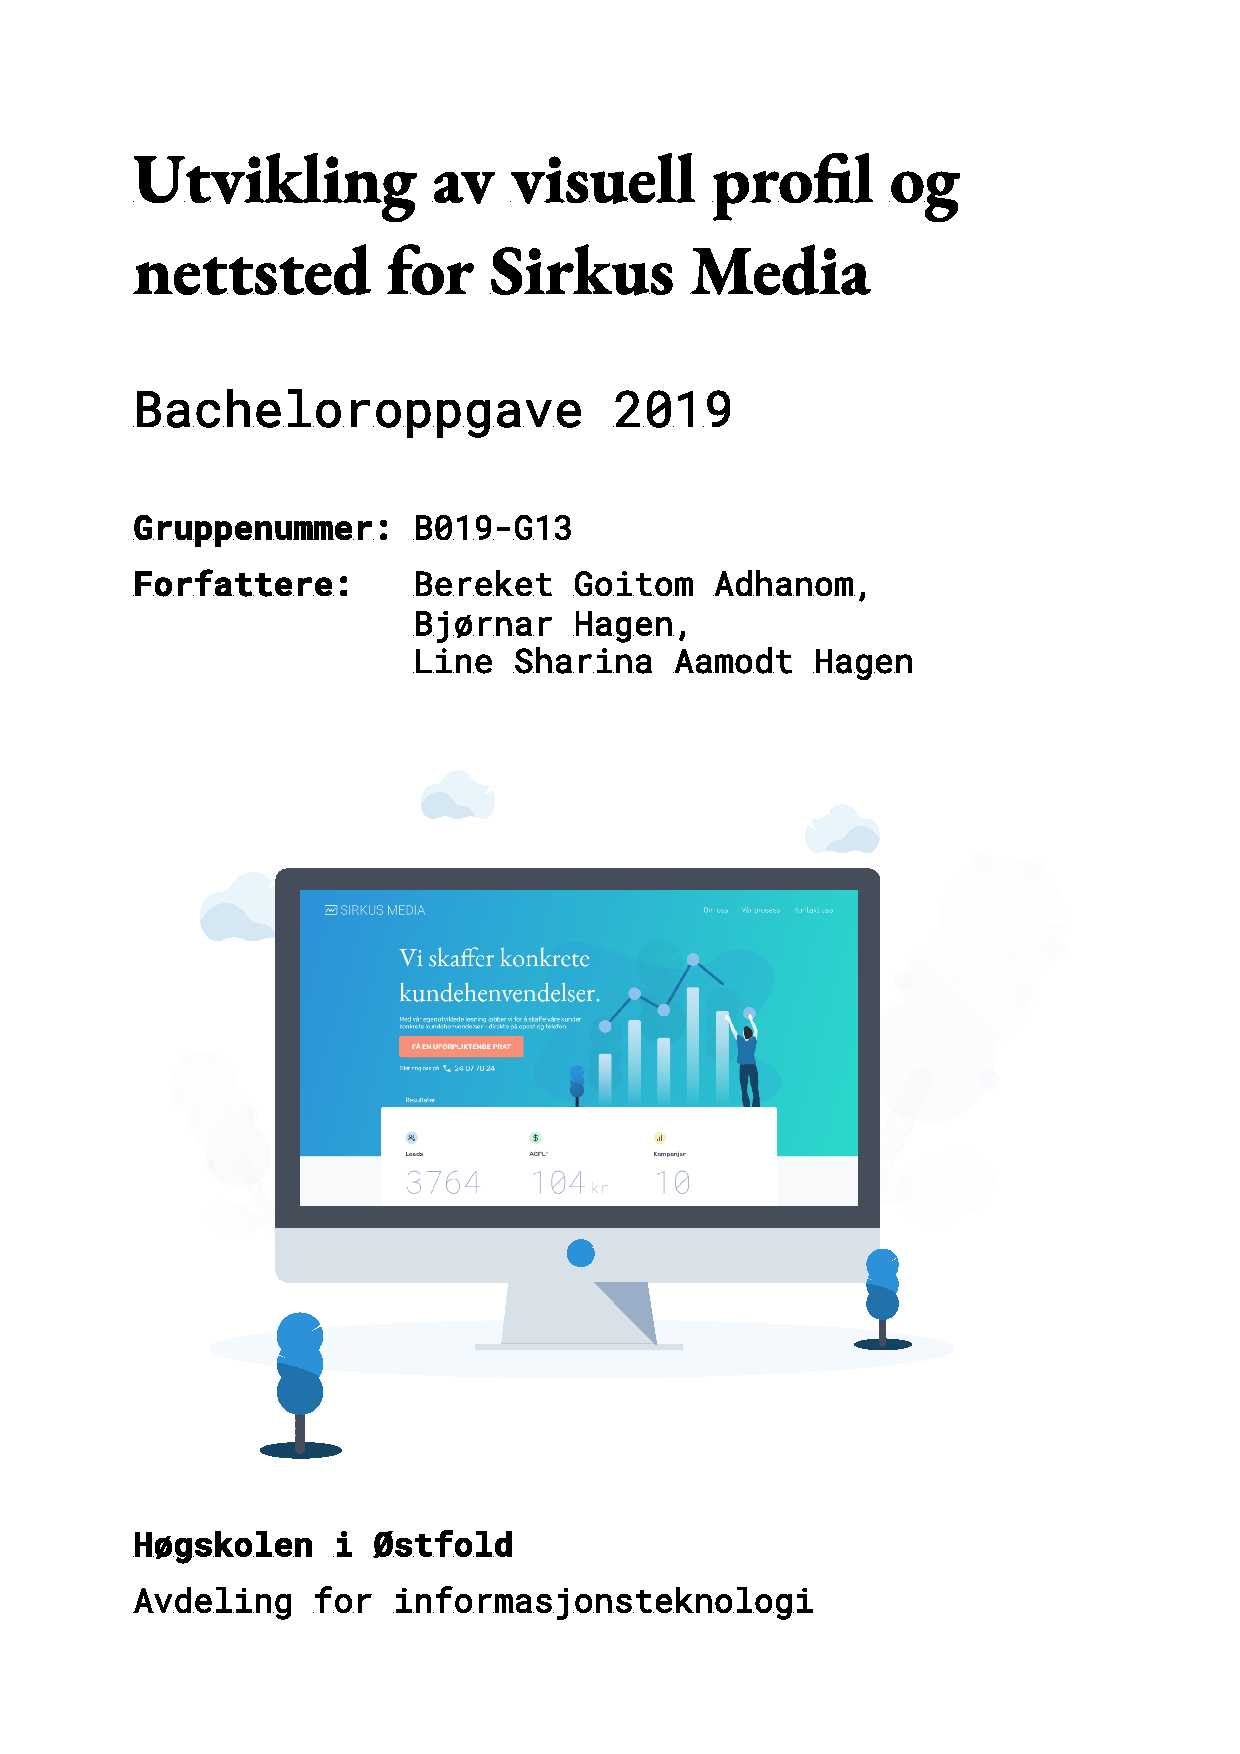
\includepdf[pages={1, {}}] {titlepage} % Make your own catchy PDF title page, named titlepage.pdf
    \maketitle
    %\cleardoublepage

\pagenumbering{roman} \setcounter{page}{-1}
\chapter*{Forord\footnote{Dette forordet skal som du skjønner ikke med i det endelige dokumentet \smiley}}

Dette er en mal beregnet til bruk i Bacheloroppgaven ved HiØ/IT. Malen gir en pekepinn om både struktur og innhold, og hvordan ting kan løses rent skriveteknisk, typisk ved å klippe og lime.

Malen er utformet som dokumentasjon på et fiktivt prosjekt, der formålet er å gjøre det lettere og enklere å dokumentere en bacheloropppgave (og liknende prosjekter). De fleste kapitler er innledet med generelle retningslinjer for hva som skal med (dette er uthevet i grått).

Det er tenkt at malen skal kunne brukes i alle de ulike prosjekttypene: utvikling, utredning og medieproduksjon. Dermed er mange overskrifter generiske, og må selvfølgelig tilpasses de enkelte prosjektene. Det kan også være aktuelt å slå sammen enkelte deler av malen, eller legge til kapitler.

Det er ikke obligatorisk å bruke malen.
 % TO BE REMOVED IN FINAL REPORT
    \cleardoublepage % TO BE REMOVED IN FINAL REPORT
    \cleardoublepage

\pagenumbering{roman} \setcounter{page}{1}
\chapter*{Sammendrag}

Sirkus Media ble stiftet i 2010 av Hans-Christian Hymer og er et teknologi-, data- og analyseselskap som leverer innovative løsninger for digital markedsføring. Deres kunder er små og store bedrifter i hele Norge som ønsker å få økt salg og lønnsomhet. 

Oppdraget går ut på å forbedre profilen til Sirkus Media på nett, slik at potensielle kunder får en bedre forståelse av deres produkter og tjenester og tar kontakt gjennom nettstedet. Dette er viktig for oppdragsgiver, ettersom dagens nettsted har store mangler og ikke inneholder nok informasjon om hva Sirkus Media tilbyr. Dagens nettsted fungerer dermed ikke som den gode markedsføringskanalen den potensielt kunne vært. 

Et nettsted kan nemlig ses på som et enveis onlineverktøy med høy bedriftskontroll. På en nettside har en bedrift mulighet til å bestemme innholdet og hvordan firmaet skal fremstå. Dette er en mulighet enhver bedrift burde benytte seg av, da nettstedet kan være med å forbedre og øke troverdigheten og dermed påvirke forholdet kunden har til bedriften.

I tillegg viser undersøkelser at det å benytte seg av internett har blitt et hverdagslig gjøremål for mange. Den første undersøkelsen kartla at hele 98\% av Norges befolkning hadde tilgang på internett hjemme i 2017. Videre viser en undersøkelse at hele 9 av 10 nordmenn surfet på nettet hver dag i 2017. SSB har også kartlagt  at så mange som 89\% av Norges befolkning, mellom 16-79 år, brukte internett til å søke etter informasjon om varer eller tjenester de siste tre månedene i 2018. Dette er svært relevante funn og er med å bevise hvorfor det er så viktig for en bedrift å være på internett i dag.

I dette prosjektet har vi valgt å benytte et CMS for å utvikle nettstedet, mer konkret et egenutviklet CMS basert på Laravel.

Rapporten gjennomgår hvordan vi har planlagt og utviklet CMS-et og nettstedet. I tillegg vil resultatene fra testing, evaluering og råd for eventuell videreutvikling av prosjektet bli presentert.
    \addcontentsline{toc}{chapter}{Sammendrag}
    %-------------------------------------------------

    % OPTIONAL
    %-------------------------------------------------
    \cleardoublepage
\chapter*{Takk Til}
% \meta{
% Det er vanlig, men ikke nødvendig, å nevne personer og miljøer som har hatt en positiv betydning for prosjektet, f.eks. på denne måten:
% }

% Jeg ønsker å takke gode kolleger ved Høgskolen i Østfold, Universitet i Oslo, og Høgskolen i Oslo og Akershus for interessante og fruktbare diskusjoner om utforming, gjennomføring og evaluering av bachelor- og masterprosjekter. I tillegg retter jeg en varm takk til pansermallene Ole, Dole og Doffen for uvurderlig støtte under arbeidet med prosjektet.

Her kommer vi til å takke personer og miljøer som har hatt en positiv betydning for prosjektet.
    \addcontentsline{toc}{chapter}{Takk Til}
    %-------------------------------------------------

	\cleardoublepage % DO NOT CHANGE    
	\setcounter{tocdepth}{2}
    \tableofcontents  % DO NOT CHANGE    
    \cleardoublepage % DO NOT CHANGE    
    
    % OPTIONAL
    %-------------------------------------------------
    \listoffigures
    \addcontentsline{toc}{chapter}{Figurliste}
    \cleardoublepage
    \listoftables
    \addcontentsline{toc}{chapter}{Tabelliste}
    \cleardoublepage
    \lstlistoflistings
    \addcontentsline{toc}{chapter}{Kodeliste}
    \cleardoublepage
    %-------------------------------------------------
       
    \pagenumbering{arabic} % DO NOT CHANGE, OR REMOVE IF CHANGING STYLE
    \setcounter{page}{1}       % DO NOT CHANGE, OR REMOVE IF CHANGING STYLE 		
	
% BODY
    % YOU MAY CHANGE TITLES AND ORDER (WITHIN LIMITS)
    %-------------------------------------------------
    %\clearpage

\section{Verktøy analyse}


\subsection{linux}
Linux er en åpenkilde operativsystem. Et operativsystem er programvare som administrerer alle maskinvareressursene som er tilknyttet skrivebordet eller datamaskinen. 
13

Linux har en rekke forskjellige versjoner kalt distribusjoner. De disribusjonene er Ubuntu Linux, Linux Mint, Arch Linux, Deepin, Fedora, Debian og openSUSE.

\url{http://lib.sgu.edu.vn:84/dspace/bitstream/TTHLDHSG/2808/1/Operating_System_Concepts_Essentials.pdf}

\subsection{nginx}
Nginx er et HTTP proxy program som kan håndtere høyere belastning av HTTP-forespørsler. 
Når nettstedet begynner å bli ferdig skal vi laste det opp på en server som kjører LEMP-stacken(Linux, Nginx, MariaDB og PHP). 
Vi valgte nginx for at den er raskere og klarer å håndtere høyere belastning sammenlignet med Apache ved hjelp av det samme settet av maskinvare.

\url{https://simplercloud.wordpress.com/2014/08/06/what-is-the-difference-between-lamp-stack-and-lemp-stack/}

\subsection{php}
\subsection{sessions}
\subsection{phpmyadmin}
\subsection{mariadb}
\subsection{mvc}
\subsection{symfony}
\subsection{laravel}
Siden oppdragsgiver har ikke satt noe krav til bruk av verktøy hadde vi fri om verktøy valg. Gruppen diskuterte om hvilke verktøy skulle brukes for å utføre prosjektet. Diskusjonen var om vi skulle bruke Laravel rammeverk eller Wordpress CMS (Control Management System). Begge verktøyene har sine gode og svake sider.  Etter vi så på begge verktøyene ble vi enige å bruke Laravel. Valget ble utført basert på informasjon som vi fant på nett og erfaring fra gruppemedlemmer. 

Rammeverket brukes vi for å utvikle et REST-API. 
Laravel er en åpen kilde PHP-rammeverk som brukes til å lage webapplikasjoner og andre typer nettsteder. Det er basert på Symfony. Symfony er et PHP webapplikasjonsramme og et sett med gjenbrukbare PHP-komponenter eller biblioteker. Det følger Model-view-controller (MVC) designmønsteret.  Dette er utgitt med innebygde funksjoner for autentisering, lokalisering, modeller, visninger, sesjoner, ruting og andre funksjoner som en inversjon av kontroll og et templerende system kalt Blade. Den nye funksjonen kommandolinje grensesnitt kalles artisan, innebygd støtte av database management system, støtte for håndtering hendelser og pakkesystem kalt bundler.

\url{https://www.educba.com/laravel-vs-wordpress/}

\subsubsection{Fordel}
\begin{itemize}
\item Laravel er et rammeverk og er veldig raskt.
\item Har mange funksjoner som autentisering, autorisasjon, inversjon av kontroll osv.
\item Alt kan tilpasses og styres hvordan tingene fungerer.
\item Databasen kan brukes eller utformes på egen måte.
\end{itemize}

\subsubsection{Ulemper}
\begin{itemize}
\item I Laravel må SEO definere egne ruter, og det tar mye arbeid å utvikle et nettsted som hovedsakelig er avhengig av innhold.
\item Laravel rammeverk er litt komplisert og krever mer kunnskap.
\item Laravel er mindre fleksibel for å oppdatere innholdet.
\end{itemize}

\subsection{csrf}
\subsection{CI \& CD}
\subsection{buddy.works}
\subsection{github}
 Git er et distribuert versjonskontrollsystem for sporing av versjoner av filer. Versjonskontroll er et system som registrerer endringer i en fil eller et sett med filer og man kan se endringene senere. Github er webportal for Git-repositoriene. Git lar deg spore og vert versjoner av filer på Github. Github hjelper utviklere for å samarbeide sammen offentlig eller privat.
 
\subsection{overleaf}
\subsection{ottomatik.io}

\subsection{amazon web services (AWS) S3}
\subsection{http2}
HTTP2 er en HTTP protokoll som gjør at vi trenger et SSL/TLS sertifikat for å servere nettsider over HTTPS. SSL/TLSsertifikatet kan skaffes gjennom Let’s Encrypt.  

\url{https://kinsta.com/learn/what-is-http2/}

\subsection{https}
HTTPS (Hypertext Transfer Protocol Secure) er en sikrere versjon av HTTP-protokollen som overfører data på web. HTTP er en applikasjonslagprotokoll for overføring av hypermedia dokumenter, for eksempel HTML. HTTPS-protokollen oppretter kryptert kanal mellom nettleseren og webserveren slik  kommunikasjonen blir sikkert. 

\url{https://www.rfc-editor.org/rfc/pdfrfc/rfc2616.txt.pdf}

\subsection{Let’s Encrypt}
Let’s Encrypt er en gratis og åpent sertifikatautoritet som gir X.509-sertifikater for kryptering av transportlagsikkerhet(TLS). Tjenesten leveres av Internet Security Research Group (ISRG).

\url{https://letsencrypt.org/}

\subsection{ssl/tls}
\subsection{html}
\subsection{css}
\subsection{sass}
\subsection{javascript}
\subsection{reactjs}
\subsection{axios}
\subsection{rest-api}
REST API-design (Representational State Transfer) er designet for å utnytte eksisterende protokoller. REST kan brukes over nesten hvilken som helst protokoll. Når den brukes til web-APIer benytter den vanligvis HTTP. Dette betyr at utviklere ikke trenger å installere biblioteker eller tilleggsprogramvare for å bruke REST API-design.

\url{https://www.mulesoft.com/resources/api/what-is-rest-api-design}

\subsection{Figma}
Figma er et grensesnitt design program som kjører i en nettleser. Vi skal bruke figma for å lage mockups. Med Figma har designere muligheter å dele en redigerbar design med andre. I tillegg kan designere også overføre filer til utviklere i en view-only modus. I denne modusen kan en utvikler inspisere design og eksportkode.

\url{https://www.xfive.co/blog/figma-best-designer-developer-cooperation/}

\subsection{ Google Analytics}
Google Analytics er en gratis webanalysetjeneste som gir statistikk og grunnleggende analytiske verktøy for søkemotoroptimalisering (SEO) og markedsføringsformål. Google Analytics hjelper for å måle, samle, analysere og rapportere av internettdata med hensikt å forstå og optimalisere bruken av nettet.
Når nettstedet er lansert skal vi måle trafikk og bruk av nettsidene ved hjelp av Google Analytics.

\url{https://searchbusinessanalytics.techtarget.com/definition/Google-Analytics}

\clearpage
    %%%% NOTATER %%%
% Skrive om forutsetninger?
% Vi lager et headless cms.
% Visualisere prosjektet: https://github.com/acaudwell/Gource

\clearpage


\clearpage
    %\clearpage

\section{Konkurrentanalyse}

Målet med konkurrentanalysen er å finne inspirasjon og kunnskap til nettstedet ved å se på eksisterende løsninger. Hvem er oppdragsgiver sine konkurrenter? Hvordan type løsning har disse valgt? Hvilke styrker og svakheter har løsningene? 

\subsection{Konkurrentene}
Sirkus Media har mange konkurrenter, deriblant alle firmaer som driver mediebyråvirksomhet. Etter samtale med Hans Christian Hymer \footnote{Samtale med oppdragsgiver (16.01.2019)} fikk vi oppgitt 3 bedrifter som blir ansett som Sirkus Media sine største konkurrenter. Det er følgelig disse konkurrentene vi har valgt å analysere.

\subsection{TACTIC™ Real-Time Marketing}
Nettstedet til TACTIC™ Real-Time Marketing ligger på følgende domene; https://tacticrealtime.com

BILDE

\subsubsection{Førsteinntrykk}
Førsteinntrykket er at nettstedet fremstår ryddig og profesjonelt. Det første som møter deg er et stort bakgrunnsbilde. Bilde dekker hele skjermen og har en tittel og en underoverskrift. Headeren består også av en knapp der du kan trykke på "Request a demo". Helt øverst på forsiden er logoen til Tactic og en meny. Til høyre er det en knapp som gir deg muligheten til å se på en video. 

\subsubsection{Forside og undersider}

Forsiden består av bakgrunnsbilde som inneholder logo, meny, overskrifter og en video.  
Deretter kommer det litt tekst om firmaet, informasjon om plattformen, logo av ledende  Ad-servers og DSP`s, partnerprogram og utvalgte kunder. Siden avsluttes med en "Contact us"-oss seksjon.

Nettstedet består også av følgende undersider:
\begin{itemize}
\item Platform
\item Company
\item Partners
\item Clients
\item Blog
\end{itemize}

\subsubsection{Teknisk analyse}
Bruke google lighthouse



\subsubsection{Styrker}
Førsteinntrykket er bra. Nettstedet fremstår som profesjonelt, noe som styrker inntrykket av bedriften. Nettstedet har også god oppbygning og struktur. 

\subsubsection{Svakheter}
Hele nettstedet er på engelsk i tillegg til at det er et .com-domene. Dette kan forvirre brukerne. Vanskelig å skjønne at dette er et firma som er lokalisert i Oslo. En annen svakhet er at det er lite luft rundt noen elementer, som fører til at nettstedet fremstår som kompakt og mer rotete. Det er heller ikke samme mengde luft over og under elementene. Dette er også med på å trekke ned helhetsinntrykket. Det er heller ikke mulig å bevege seg rundt på nettstedet ved hjelp av tastaturet. Dette gjør det også vanskelig å navigere seg rundt ved hjelp av skjermleser, noe som er et krav i loven om universell utforming og tilgjengelighet. I tillegg får nettstedet mange kontrastfeil \footnote{Sjekk av kontraster ble gjort med hjelp av http://wave.webaim.org,}, som også bryter kravet om universell utforming.

\subsection{Marketer Technologies AS}
Nettstedet til Marketer Technologies AS ligger på følgende domene;
https://marketer.tech/

\subsubsection{Førsteinntrykk}
Førsteinntrykket av nettstedet er positivt, fordi den fremstår som ryddig og profesjonell. Det første som møter deg er logoen til firmaet og en meny. Under menyen er en tittel, en underoverskrift og to lenker. Får også opp et ikon for chat. Det at man enkelt kan ta kontakt kan for en kunde virke betryggende, og kan være med å øke troverdigheten til bedriften.

BILDE

\subsubsection{Forside og undersider}

Nettstedet består også av følgende undersider:
\begin{itemize}
\item Solutions
\item Company
\item Customers
\item Blog
\item Careers 
\item Contact
\item Book demo
\end{itemize}

\subsubsection{Teknisk analyse}

\subsubsection{Styrker}
Bra førsteinntrykk. De har chat. Nettsted som skiller seg ut. Gjennomført.

\subsubsection{Svakheter}



\subsection{Inviso AS}
Nettstedet til Inviso AS ligger på følgende domene;
https://www.inviso.no/

\subsubsection{Førsteinntrykk}
Førsteinntrykket av nettstedet er at den fremstår som rotete. Hovedgrunnen til dette er at det er mange elementer og mye som skjer i headeren. Logoen og noe av teksten på bakgrunnsbilde er også vanskelig å se, på grunn av for dårlig kontrast. 

\subsubsection{Forside og undersider}

Nettstedet består også av følgende undersider:
\begin{itemize}
\item Inviso
\item Våre produkter
\item Kontakt
\item Galleri
\item Verktøy
\item Nyheter
\end{itemize}


\subsubsection{Teknisk analyse}

\subsubsection{Styrker}

\subsubsection{Svakheter}

\subsection{Konklusjon}

Burde også presentere sine kunder. Dette er tillitsvekkende og fører til bedre troverdighet.

\clearpage
    \cleardoublepage
\chapter{Introduksjon}
\label{chap:intro}
Kapittel 1 omhandler rammene rundt prosjektet, prosjektets formål metoder og leveranser. Her vil også oppdragsgiver og studengruppen bli presentert. Prosjektet er knyttet til Bacheloroppgave 2019, der oppdragsgiveren er Sirkus Media. Veileder for prosjektgruppen er Einar Krogh. 

\section{Prosjektgruppen}

Prosjektgruppen består av 3 medlemmer, der alle er dataingeniørstudenter. Gruppen ble allerede kjent på sommerkurset knyttet til Y-veien, og har tidligere samarbeidet på flere gruppeprosjekter gjennom hele studietiden. Allerede første år på studiet fant vi ut at vi samarbeidet godt, en faktor som var viktig for alle deltagerne på gruppen når det skulle dannes bachelorgruppe. Kompetansemessig utfyller gruppen hverandre godt, da alle har forskjellige områder og teknologier som foretrekkes å jobbe og lære mer om.  

\subsection{Om Bereket}
Gikk på IKT-servicefag på  videregående og var deretter lærling hos IT-avdelingen til Rana kommune. Etter bestått fagbrev begynte jeg på Høgskolen i Østfold på dataingeniørstudiet Y-vei.

Er interessert å jobbe med teknologier som HTML, CSS, PHP og JavaScript.

\subsection{Om Bjørnar}
Tok fagbrev som IKT-servicemedarbeider hos Optimale Systemer AS i Larvik etter 2 år som lærling. Dette etter å ha fullført IKT-linja hos Sandefjord videregående skole. Deretter gikk det videre til Høgskolen i Østfold, og startet da på Y-veien for dataingeniørstudiet.

Jobber nå som daglig leder hos Datahjelpen AS, hvor arbeidsoppgavene innebærer utvikling som full-stack og en del DevOps. Liker å jobbe med teknologier som HTML, CSS, JavaScript, Node, React, PHP og Linux.

\subsection{Om Line}
Gikk IKT-servicefag på Sandefjord videregående skole. Var etter dette lærling hos Vestfold Fylkeskommune der jeg tok fagbrev og dermed ble utdannet IKT-servicemedarbeider. Startet deretter på Y-veien på dataingeniørstudiet ved Høgskolen i Østfold. Har alltid vært interessert i data og teknologi, og skjønte tidlig at dette var noe jeg ønsket å jobbe med.

Jobber nå som front-end utvikler hos Datahjelpen AS og liker best å jobbe med teknologier som HTML, CSS, JavaScript og PHP.

\section{Oppdragsgiver}
Oppdragsgiver for dette prosjektet er Sirkus Media.
Sirkus Media ble stiftet i 2010 av Hans-Christian Hymer og er et teknologi-, data- og analyseselskap som leverer innovative løsninger for digital markedsføring. Deres kunder er små og store bedrifter i hele Norge som ønsker å få økt salg og lønnsomhet. 

Ved hjelp av deres egenutviklede løsning jobber de med å skaffe konkrete kundehenvendelser til sine kunder. Løsningen når direkte ut til kjøpsklare kunder. Dette innebærer at de utelukkende markedsfører mot personer som, basert på nettadferd, vet at med stor sannsynlighet er på utkikk etter produkter eller tjenester som selskapet tilbyr.

Sirkus Media har i dag 2 ansatte og hadde i 2017 en omsetning på 6.4 millioner\footnote{\url{https://www.proff.no/bransjes\%C3\%B8k?q=sirkus\%20media}}.
Vår kontaktperson hos oppdragsgiver er Hans-Christian Hymer som både er grunnlegger og daglig leder av Sirkus Media. 

\section{Oppdraget}
\label{sec:oppgaven}
Bakgrunnen for dette prosjektet er at Sirkus Media ønsker å forbedre deres profil på nett, slik at potensielle kunder får en bedre forståelse av deres produkter og tjenester og tar kontakt gjennom nettstedet. Dette er viktig for oppdragsgiver ettersom dagens nettsted har store mangler og ikke inneholder nok informasjon om hva Sirkus Media tilbyr. Dagens nettsted fungerer dermed ikke som den gode markedsføringskanalen den potensielt kunne vært. Sirkus Media har derfor et stort behov for utvikling av en ny nettside. 

Det er et krav at nettstedet skal følge gjeldende lover og regler i Norge, særlig med tanke på universell utforming og personvern. I tillegg bør nettstedet implementeres med beste praksis for søkemotoroptimlisering, struktur og semantikk. Det skal også være mulig å bruke nettstedet på de fleste type plattformer og enheter. Minstekravet er at nettsiden er tilpasset og funksjonell for mobil, nettbrett, MacOS, Linux og Windows.

I tillegg til nettstedet omfatter oppgaven: 
\begin{itemize}
\item Analysering av nåværende løsning, konkurrenter og passende verktøy
\item Utforming av logo, skisser, visuell profil og designsystem
\item Planlegging og oppretting av database
\item Analysering av ferdig produkt
\item Dokumentasjon og brukerveiledninger til oppdragsgiver
\end{itemize}

\section{Hvorfor, hva og hvordan: Formål, leveranser og metode}
\label{sec:maal-metode-resultater}
\subsection{Formål}
\label{sec:maal}
\begin{compactitem}
\item [{\bf Hovedmål}] Forbedre Sirkus Media sin profil på nett, slik at potensielle kunder får en bedre forståelse av deres produkter og tjenester og dermed tar kontakt gjennom deres nettsted. På et overordnet plan vil dette bidra til å øke omsetningen til oppdragsgiver.
\begin{compactitem}
\item [{\bf  Delmål 1} ] Generere mer trafikk, som fører til at flere kunder tar kontakt med bedriften. 
\item [{\bf  Delmål 2} ] Måle trafikken på nettstedet, slik at man ser hva som fungerer og deretter kan tilpasse informasjonen til brukerne som besøker siden.
\end{compactitem}
\end{compactitem}

\subsection{Leveranser}
\label{sec:resultater}
Hovedresultatet til dette prosjektet vil være et komplett og offentlig nettsted, som er tilgjengelig på Sirkus Media sitt domene.

% Bacheloroppgaven har i tillegg noen krav til leveranser og følgende dokumenter må derfor leveres:
%\begin{itemize}
%\item Prosjekt og gruppekontrakt
%\item Gruppenettsted
%\item Forprosjektrapport
%\item Første versjon av hoveddokument
%\item Andre versjon av hoveddokument
%\item Hoveddokument med vedlegg
%\item Prosjektplakat
%\item Presentasjon
%\end{itemize}

I tillegg til leveranser knyttet til bachelorprosjektet, vil disse konkrete resultatene bli opprettet underveis i prosjektperioden:
\begin{itemize}
\item Analyse av gammelt nettsted
\item Analyse av konkurrenter
\item Analyse av verktøy
\item Visuell profil og designsystem
\item Prototype og mockups av nytt nettsted
\item Database og modeller
\item Analyse av nytt nettsted
\item Sitemap
\item Brukerveiledninger
\end{itemize}

\subsection{Metode}
\label{sec:metode}
For å oppnå både hovedmål og delmål må gruppen gjøre noen tiltak. Hovedmålet, som beskrevet tidligere, er å forbedre Sirkus Media sin nettprofil. Dette løser vi med å analysere dagens nettside og kartlegger hva som er bra og dårlig. Deretter går vi videre til å analysere konkurrentene sine nettsider og ser hvordan deres løsninger ser ut. Denne analyseringen kan gi oss inspirasjon til vår løsning, men også hint på hva vi ikke burde gjøre.

Det første delmålet som skal oppnås er å generere mer trafikk til nettsiden. Da må vi å lage et attraktivt nettsted som følger beste praksis for god søkemotoroptimalisering, semantikk og universell utforming. Disse tre faktorene er sterkt knyttet sammen, da både god semantikk og universell utforming vil forbedre søkemotoroptimaliseringen. God søkemotoroptimalisering er viktig når kundene skal finne en bedrift.

For å oppnå delmålet om måling av trafikk på nettstedet må vi benytte oss av verktøy som Google Analytics. Dette gir oss en komplett oversikt over trafikk og brukermønster.

Mockups oppnår vi ved å hente inspirasjon fra lignende nettsider og deretter lager et forslag på design til nettstedet. Før utviklingen av nettstedet begynner , må designforslaget blitt godkjent av oppdragsgiver.

Database og modeller løser vi ved å først tegne og deretter forbedre databasen ved hjelp av penn og papir. Deretter opprettes et UML-diagram digitalt.

\section{Rapportstruktur}

% \meta{
% Det er vanlig å avslutte innledningen med en oversikt over resten av rapporten, f.eks. slik som dette:
% }

% I Kapittel~\ref{chap:analysis} starter vi med å se på generelle krav til akademiske og tekniske dokumenter, og ikke minst hva som skiller disse fra ``vanlige'' dokumenter. Vi ser deretter nærmere på krav og retningslinjer til bachelorrapporter ved nasjonale og internasjonale læresteder. Vi går også gjennom HiØ/IT sine egen beskrivelse av hovedprosjektet.  Vi gir eksempler på maler fra andre læresteder. Deretter ser vi på de tekniske sidene ved å produsere store og komplekse dokumenter, med spesiell vekt på aktuelle programvareverktøy. Vi presenterer en overordnet design av vår rapportmal i Kapittel~\ref{chap:design}, og beskriver den konkrete implementasjon i OpenOffice i Kapittel~\ref{chap:implementation}. Løsningen blir ad-hoc evaluert i Kapittel~\ref{chap:evaluation}, og i Kapittel~\ref{chap:discussion} diskuterer vi resultatet av prosjektet. Rapporten avsluttes med en kort konklusjon i Kapittel~\ref{chap:conclusion}. En mer detaljert gjennomgang av hvordan malen kan brukes finnes i Vedlegg~ \ref{chap:how-to}.

I Kapittel~\ref{chap:analysis} starter vi med å se på relevant teori og beste praksis for planlegging, design og utvikling. Dette gjør at vi kan begynne å danne oss et bilde av hvordan et nettsted bør se ut. I Kapittel~\ref{chap:design} tar vi for oss hvordan vi faktisk har tenkt til å utforme nettstedet, og kommer til å være selve grunnlaget for utviklingen. Kapittel~\ref{chap:implementation} beskriver den konkrete implementasjonen av nettstedet. Deretter vil løsningen bli testet både teknisk, av utvalgte brukere og av oppdragsgiver i Kapittel~\ref{chap:evaluation}. I Kapittel~\ref{chap:discussion} diskuterer vi resultatet av prosjektet, og rapporten avsluttes med en kort konklusjon i Kapittel~\ref{chap:conclusion}.

    \cleardoublepage
\chapter{Analyse og teori}
\label{chap:analysis}
\meta{
Kapittelet tar for seg analysedelen av arbeidet. Den består av to hoveddeler, en grundig beskrivelse av oppgaven basert på skissen gitt av oppdragsgiver, og en undersøkelse av hva som finnes av relatert arbeid, {\em best practise} og relevant teknologi. 
}

I dette kapittelet danner vi oss et bilde av hvordan en akademisk/teknisk rapport bør se ut, både med hensyn på innhold, struktur og utforming. Vi ser også på hvordan store og komplekse dokumenter blir produsert (både analogt og digitalt), og hva slags (digitale) verktøy som kan tenkes å brukes. Vi går også gjennom endel tilgjengelig materiale som kan gjøre det lettere å velge hva slags digitale verktøy man burde bruke i en bacheloroppgave\footnote{Utvalget er noe overfladisk utført, i hovedsak basert på forfatterens erfaringer.}.

-- 

Kapittel 2 omhandler relevant teori og beste praksis for planlegging, design og utvikling. I dette kapittelet vil vi danne oss et bilde av hvordan en nettsted bør se ut. Både med hensyn på innhold, struktur og utforming. I tillegg vil vi presentere de verktøy vi mener er passende i et slikt prosjekt.

\section{Utdypning av oppgavebeskrivelse}
Sirkus Media har gitt utrykk for at de ønsker en "one-pager". Dette vil si at nettstedet i hovedsak består av en langt nettside. Samtidig ønsker oppdragsgiver at nettstedet skal være godt synlig i Google og andre søkemotorer og at det finnes mulighet for innlogging slik at det er mulig å legge til, oppdatere og fjerne innhold. Studengruppen vil dermed utvikle et eget CMS eller benytte et ferdigutviklet system som møter disse behovene. 

CMS og API

\section{Risikoanalyse}

\section{Hvorfor et nettsted er viktig}
Å benytte seg av internett har i dagens samfunn blitt et hverdagslig gjøremål for mange. I følge undersøkelser gjort av Statistisk sentralbyrå (SSB)\footnote{Statistisk sentralbyrå utarbeider og gir ut offisiell statistikk i Norge} i 2017, hadde hele 98\% av Norges befolkning tilgang på internett hjemme \cite{ssb17fim}. Det viste seg også at 9 av 10 nordmenn surfet på nettet hver dag \cite{ssb17nat}. SSB har også kartlagt  at så mange som 89\% av Norges befolkning, mellom 16-79 år, brukte internett til å søke etter informasjon om varer eller tjenester de siste 3 måneder i 2018 \cite{ssb18aup}. Disse foregående funnene er svært relevante, og er med å underbygge hvorfor det er så viktig for en bedrift å være på internett i dag.

I tillegg til disse funnene, er det også andre faktorer som bidrar til at et nettsted for en bedrift er så viktig i dag. Disse blir presentert nærmere i dette kapittelet. 

\subsection{Treff i søk}
Når en bedrift har et nettsted blir det mulig å dukke opp i søkeresultatene hos søkemotorer\footnote{Se avsnitt \ref{sec:concepts-seo}}. I følge undersøkelser gjort av Google viser det seg at hele 76\% av de som søker på smarttelefonene etter noe i nærheten, besøker en bedrift innen en dag \cite{google16hms}. I tillegg viser undersøkelsene at når et spørsmål eller behov oppstår er sannsynligheten minst dobbelt så stor for å benytte seg av søk, enn andre online og offline kilder som sosiale medier eller å besøke butikker. Ikke bare er søk den mest brukte ressursen, det er den tjenesten 87\% vender seg til først \cite{google16mhc}. I undersøkelsene ble det også kartlagt at 51\% av brukere har oppdaget et nytt produkt eller bedrift når de har utført søk på deres telefon \cite{google16scp}. For bedrifter er det altså helt avgjørende å være godt synlig hos søkemotorer.




\subsection{Troverdighet}
\label{sec:analyse-troverdighet}
Etter studier gjort av avdelingen for informasjon og ledelse ved HuaZhong Normal University viser det seg at troverdihgeten til en bedrift sitt nettsted er en viktig faktor når brukerene skal bestemme seg for om prosessen skal gå videre eller ikke, og vil ha en stor påvirkning på deres avgjørelse når det gjelder kjøp.


\meta{The level of enterprise website credibility is an important basis for the
website browsers (or consumers) deciding whether to take
further action or not, and will have a great influence on their
purchase decision-making. }

I følge studiene kommer det også frem at kriteriene for å bestemme troverdigheten til et nettsted er basert på subjektiv vurdering og ikke profesjonell analyse. Brukere undersøker vanligvis utseende, informasjon og funksjon til nettstedet i henhold til deres faktiske behov og gjør seg deretter opp deres egen konklusjon \cite{zhao2009eew}.

\meta{As the above study shows, criterion for determining the
credibility of website is based on subjective judgment instead
of professional analysis. People usually examine the
appearance, information and function of the website
according to their actual needs and then get their own
conclusion.}
% https://ieeexplore.ieee.org/stamp/stamp.jsp?tp=&arnumber=5279898


I en studie gjennomført av BrightLocal Ltd. i 2016 ble det gjort undersøkelser på hva forbrukere ønsker fra lokale bedrifter. Resultatene ble tatt fra et panel på 800 forbrukere, der alle er basert i USA, med forskjellig alder og kjønn. Blant de 800 respondentene, var alderspennet følgende: 

\begin{itemize}
\item 18-34 – 44\%
\item 35-54 – 34\%
\item 55+ – 22\%
\end{itemize}

I denne undersøkelsen svarte 40\% av aldergruppen mellom 18-34 og 35-54 at det er mer sannsynlig at de kontakter en lokal bedrift hvis de har en nettside. På spørsmål om en klar og smart nettside øker bedriftens troverdighet, svarte 43\% av respondendene over 55 at dette hadde noe å si \cite{marchant18wdc}.

Med utgangspunktet i disse studiene kan vi derfor konkludere med at en nettside med god troverdighet kan føre til at flere potensielle kunder tar kontakt.

\subsection{Markedsføringskanal}
Nettstederer er et eksempel på et enveis nettverktøy med høy  bedrifts kontroll.
Websites and e-mail can be seen as examples of one-way online tools with high company control. https://www.emeraldinsight.com/doi/pdfplus/10.1108/JSBED-05-2013-0073. På en nettside har en bedrift altså mulighet til å bestemme innholdet og hvordan firmaet skal fremstå. Dette er en mulighet enhver bedrift burde benytte seg av, da nettstedet kan være med å forbedre og øke troverdigheten\footnote{Se avsnitt \ref{sec:analyse-troverdighet}} og dermed forholdet kunden har til bedriften.

\subsection{Innsamling av data}
En annen god grunn for å ha et nettsted, er at man kan benytte seg av verktøy som Google Analytics\footnote{Se avsnitt \ref{sec:google-analytics}}. Data samlet av Google Analytics kan brukes til å finne ut av hvilken av sidene som er mest populær eller har flest besøk. Det er også mulig å finne ut av hvilken type informasjon besøkene er interessert i, gjennom hvilken vei en bruker kommer inn og ut av siden på og hvor mye tid som har blitt brukt på nettstedet \cite{kent2011lwa}. Ved å kartlegge dette vil bedriften alltid ha oppdatert og relevant informasjon tilgjengelig, som kan brukes til å forbedre nettstedet fortløpende. 

% https://ac.els-cdn.com/S0363811111001433/1-s2.0-S0363811111001433-main.pdf?_tid=6362f9f9-b2cf-4c0f-95ac-004f5552c93e&acdnat=1550673249_e4d9b2b5340feb6427e7bd538ecd0f65


\section{Viktige faktorer innen webdesign}
Innenfor webdesign finnes det flere forskjellige faktorer er avgjørende når det kommer til hvor godt et nettsted er utført. En presentasjon av disse faktorene og hvorfor de er så viktig vil bli presentert nærmere i dette kapittelet. 

\subsection{Målgruppe}

\url{https://www.thinkwithgoogle.com/marketing-resources/tutorials/human-insights-audience-strategy/}

En målgruppe


\subsection{Design, profil og førsteinntrykk}
\url{https://www.tandfonline.com/doi/pdf/10.1080/10447318.2013.839899?needAccess=true }

\url{http://news.mst.edu/2012/02/eye-tracking_studies_show_firs/}

\url{https://www.tandfonline.com/doi/abs/10.1080/01449290500330448 }


\subsection{Responsivt design}
Undersøkelser fra Google om mobilbruk... Står om det i en av kildene som har blitt brukt tidligere

\subsection{Søkemotoroptimalisering}
\label{sec:concepts-seo}
Søkemotoroptimalisering (SEO) går ut på å oppnå gode plasseringer i de organiske søkeresulatene hos søkemotorer \cite[s.~16]{flensted10smg}. I praksis handler SEO om at en nettside blir optimalisert på en rekke områder, slik at søkemotoren finner akkurat dette nettstedet og presenterer den godt synlig i de organiske søkeresultatene ved å se på søkeordene ønsket målgruppe benytter  \cite[s.~20]{flensted10smg}.

Mer teoretisk fungerer søkemotoroptimalisering ved at de innsamlede dataene blir indeksert og lagret. Alle disse operasjonene utføres av søkemotorprogramvaren (crawler, edderkopp,
bot). Disse programmene beveger seg ved å bruke hyperkobling struktur på nettet. De navigerer regelmessig gjennom nettsider og fanger endringer som har blitt gjort siden sist  \cite[s.~488]{yalccin2010search}.

Undersøkelser viser at 75\% of Internet users never scroll past the first page of search results, TRENGER KILDE!! 
Disse funnene underbygger påstanden om at SEO er viktig i dagens samfunn, og en god SEO-strategi er derfor på sin plass. 
\url{https://www.searchenginepeople.com/blog/40-unbelievable-seo-statistics-need-know.html#note-68961-5 }

En faktor som er viktg å tenke på er at god SEO krever disiplin, planlegging og research før man setter i gang. Dette er ikke en oppgave som kun gjøres en gang, og krever konstant overvåking og optimalisering da algoritmene hele tiden endrer hvordan de evaluerer nettsider \cite[s.~1]{mitchell2012usb}. Derfor er det viktig å hele tiden ha SEO i fokus når man utvikler, når et av målene er god plassering hos søkemotorene.


\subsection{Brukeropplevelsen}
I følge Steve Krug, forfatteren bak boken \q{Don't make me think}, går brukervennlighet ut på noe så enkelt som at en helt vanlig bruker med gjennomsnittlige egenskaper og erfaring (eller til og med lavere), skal kunne finne ut av hvordan en ting skal brukes for å oppnå et mål, uten å dette fører til mer trøbbel enn det er verdt \cite[s.~9]{krug2014dmt}. Det er nettopp derfor forfatterens første lov til god brukeropplevelse er \q{ikke få meg til å tenke}. Et nettsted bør nemlig være selvforklarende, og en bruker skal intuitivt forstå hva et nettsted representerer og hvordan den kan brukes, uten å måtte anstrenge seg for å finne ut av det \cite[s.~11]{krug2014dmt}. Krug hevder at dette er viktig, fordi brukere kan tenke at det faktum at utviklerne bak dette nettstedet ikke tok seg bryet med å gjøre ting åpenbart og enkelt, vil påvirke deres inntrykk av siden og hele bedriften bak den \cite[s.~15]{krug2014dmt}.

\url{https://www.thinkwithgoogle.com/marketing-resources/experience-design/strong-audience-design/}

\subsubsection{Hastighet}

Bouncerate 
\url{https://www.section.io/blog/page-load-time-bounce-rate/ }


\section{Lovverk}
Det finnes også noen lovverk som må følges når det kommer til utvikling av nettsteder. I dette underkapittelet blir det beskrevet hva disse går ut på. Det blir også gjennomgått hvorfor disse lovene er viktig, utover det faktum at de er lovpålagt. 

\subsection{WCAG 2.0}

\subsection{GDPR}



\section{Beste praksis og tidligere undersøkelser}
Undersøkelser viser at følgende struktur på en nettside er å foretrekke...:

Finne et nettsted som følger best practice og skrive om det.

Obvious Always Wins:
\url{https://www.lukew.com/ff/entry.asp?1945}

\subsection{Innhold}
https://www.brightlocal.com/2016/03/04/gender-age-what-consumers-want-from-local-business-websites/ 
\subsection{Struktur}

\subsection{Sikkerhet}
 (hashing av passord. sende data over kryptert kanal)

\section{Analyse av opprinnelig løsning}

Målet med å analysere det nåværende nettstedet til Sirkus Media er å kartlegge eventuelle problemerområder som burde forbedres. Når utviklingen av det nye nettstedet er ferdig vil vi sammenligne de nye testresultatene med resultatene som blir presentert i dette kapittelet.
Se figur \ref{fig:analysis-current-sirkusmedia.no} for bilde av nettsiden på PC og mobil.

\begin{figure}[H]
    \begin{center}
        \subfigure[PC]{
            \label{fig:analysis-current-sirkusmedia.no-desktop}
            \frame{
\includegraphics[width=0.7\textwidth]{bjornar/sirkusmedia_no_(1366x768).png}}
        }
        \subfigure[Mobil]{
            \label{fig:analysis-current-sirkusmedia.no-mobile}
            \frame{
\includegraphics[width=0.25\textwidth]{bjornar/sirkusmedia_no_(iPhone_6_7_8).png}}
        }
        \label{fig:analysis-current-sirkusmedia.no}
        \caption{sirkusmedia.no}
    \end{center}
\end{figure}

\subsection{Test med Google Chrome DevTools}
Google Chrome DevTools\footnote{\url{https://developers.google.com/web/tools/chrome-devtools/}} er et utviklerverktøy som følger med nettleseren Google Chrome. Det lar oss blant annet sjekke hastighet og kontrastforhold på siden og kjøre tester med Google Lighthouse.

Vi testet hastigheten til siden på det trådløse nettverket til Høgskolen i Østfold (avdeling Halden) fra en Dell XPS 13 (9350).
Resultatene måles i millisekunder.

\begin{table}[H]
\begin{tabular}{lllll}
Test & DOM & Load &  &  \\
1 & 268 & 624 &  &  \\
2 & 203 & 550 &  &  \\
3 & 216 & 560 &  &  \\
4 & 387 & 928 &  &  \\
5 & 210 & 572 &  &  \\
6 & 634 & 844 &  &  \\
7 & 309 & 857 &  &  \\
8 & 256 & 670 &  &  \\
9 & 348 & 673 &  &  \\
10 & 249 & 579 &  &  \\
\end{tabular}
\end{table}

Gjennomsnitt:\\
- DOM: 308ms\\
- Load: 614ms

Innlastningstiden til DOM beskriver hvor lang tid det tar for nettleseren å lese gjennom og analysere HTML-koden til nettsiden. Load vil si hvor lang tid det tar å laste inn DOM sammen med alle bilder, stylesheets, scripts og iframes.

\subsection{Test med Google Lighthouse}
\label{sec:analysis-current-lighthouse}

Ved å kjøre Google Lighthouse får vi resultater for hastighet, tilgjengelighet, beste praksis, søkemotoroptimalisering og progressiv webapplikasjon. Figur \ref{fig:analysis-current-lightouse-summary} viser oppsummering av resultatetene etter å ha kjørt testen. Oversikten viser at nettstedet får gode poengsummer på alle områdene. Hovedgrunnen til dette er at dagens nettsted består av kun en forside og lite informasjon. Dette begrenser muligheten for feil.

\begin{figure}[H]
    \centering
    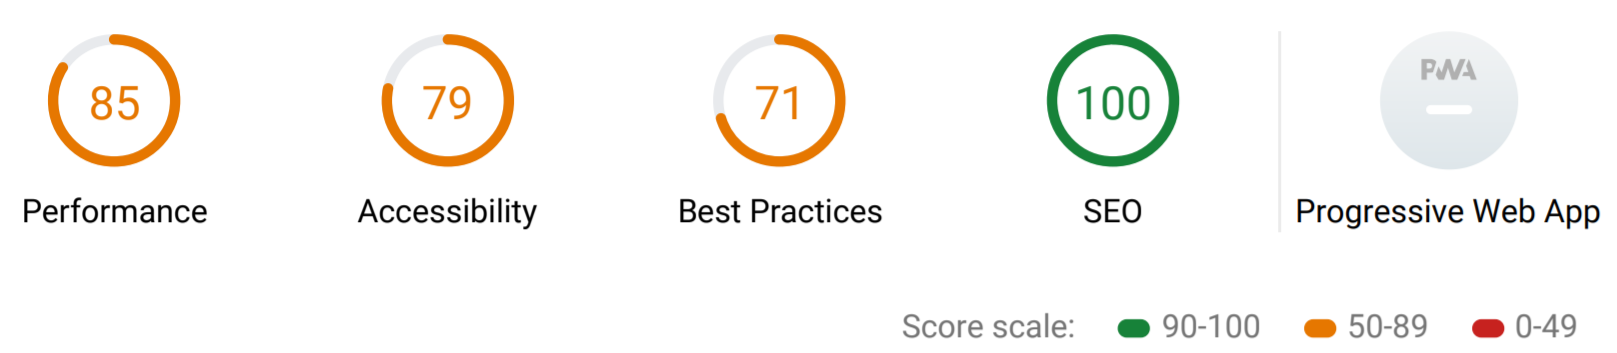
\includegraphics[width=\textwidth]{bjornar/Lighthouse-Report-mobile.png}
    \caption{Resultater fra Google Lighthouse}
    \label{fig:analysis-current-lightouse-summary}
\end{figure}

Ikonet for \q{Progressive Web App} har en feil, slik at man ikke får sett scoren. Ved hjelp av en JSON-fil\footnote{Se JSON-fil, linje 3386} som inneholder resultatene, ser man at poengscoren er på 58\%.

Denne delen av testen er egentlig ikke relevant\footnote{Sirkus Media sitt nettsted er ikke, og kommer ikke til å bli en progressiv webapplikasjon. KILDE OM PWA}, og vi vil derfor ikke se på denne, eller nevne den i andre tekniske analysener som bruker Google Lighthouse.

I rapporten kan vi se at Google laster inn nettsiden på 2,7 sekunder og at det tar 4,9 sekunder før siden blir beregnet som interaktiv. Hovedproblemet til siden er bruken av \q{render-blocking resources}\footnote{Hva er dette?}. Dette kan lett fikses og kan i følge Google spare 1,34 sekunder. Google påpeker også at det finnes 3 sikkerhetshull i JavaScript-biblioteker som blir brukt på nettsiden. Dette er ikke ønskelig, da dette øker risikoen for uønskede hendelser.

Full rapport for Google Lighthouse testen kan leses i vedlegg X.

\subsection{Checkbot}
\begin{figure}[H]
    \centering
    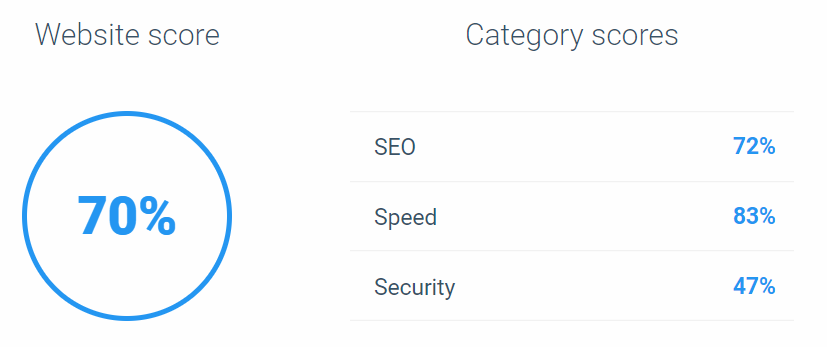
\includegraphics[width=0.75\textwidth]{bjornar/checkbotio-summary.png}
    \caption{Checkbot.io summary}
    \label{fig:analysis-current-checkbot-summary}
\end{figure}

Checkbot\footnote{https://checkbot.io} tester sikkerhet, hurtighet og søkemotoroptimalisering. Figur \ref{fig:analysis-current-checkbot-summary} viser oppsummering av resultatene. En mer detaljert rapport kan leses under vedlegg X. Denne testen viser en god poengsum når det gjelder totalt for gjennomsnittet. Isolert sett ser vi at sikkerheten til nettstedet drar ned gjennomsnittet betydlig. Den fulle rapporten viser at dette kommer av at nettsiden ikke bruker HSTS, \q{content sniffing protection}, \q{clickjack protection}, \q{XSS protection} og at det ikke skjuler server-versjon data.

\subsection{Color Contrast Analyzer}
\label{sec:analysis-current-color-contrast-analyzer}
Color Contrast Analyzer\footnote{\url{https://accessibility.oit.ncsu.edu/tools/color-contrast-chrome/}} tar bilde av nettstedet og scanner deretter kontrasten. Områder med bedre kontrast utheves og får lyse kanter. Jo mer markante kanter, desto mer kontrast.

\begin{figure}[H]
    \centering
    \makebox[\textwidth]{
\includegraphics[width=0.80\paperwidth]{bjornar/contrast-wcag-aa-small.png}}
    \caption{CCA resultat AA}
    \label{fig:analysis-current-cca-aa}
\end{figure}

\begin{figure}[H]
    \centering
    \makebox[\textwidth]{
\includegraphics[width=0.80\paperwidth]{bjornar/contrast-wcag-aaa-small.png}}
    \caption{CCA resultat AAA}
    \label{fig:analysis-current-cca-aaa}
\end{figure}

Ved å kjøre testen \q{small non bold text} for nivå AA, som gjelder for skriftstørrelser opptil 18pt, viser resultatene at deler av teksten i logo og de grønne overskriftene ikke har gode nok kontraster. Dette illustreres i figur \ref{fig:analysis-current-cca-aa}. Google Chrome DevTools verifiserer at kontrastforholdet ikke oppfyller kontrastkravet for AA. Se figur \ref{fig:analysis-current-cdt-a} og \ref{fig:analysis-current-cdt-b}

\begin{figure}[H]
    \begin{center}
        \subfigure[grønn overskrift]{\label{fig:analysis-current-cdt-a}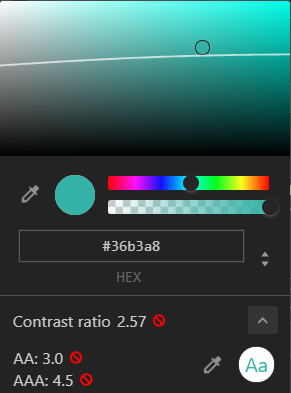
\includegraphics[width=0.3\textwidth]{bjornar/contrast-wcag-aa-small-gronn-tekst.png}}
        \subfigure[blå tekst i logo]{\label{fig:analysis-current-cdt-b}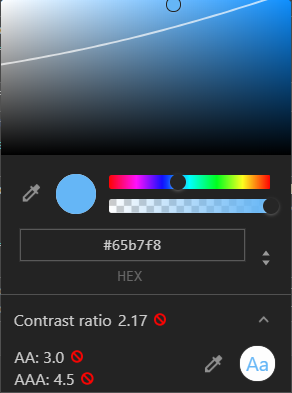
\includegraphics[width=0.3\textwidth]{bjornar/contrast-wcag-aa-small-logo-blaa.png}}
        \subfigure[vanlig tekst]{\label{fig:analysis-current-cdt-c}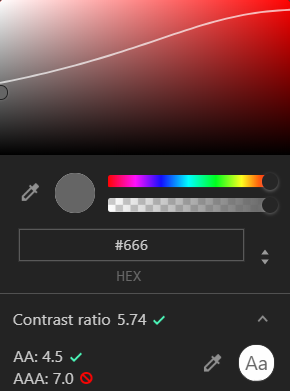
\includegraphics[width=0.3\textwidth]{bjornar/contrast-wcag-aaa-small-body.png}}
        \caption{Google Chrome DevTools - kontrastforhold}
        \label{fig:analysis-current-cdt}
    \end{center}
\end{figure}

Resultatene etter å ha kjørt tester for nivå AAA viser at mesteparten av nettstedet ikke oppfyller kravet for kontrastnivå. Se figur \ref{fig:analysis-current-cca-aaa}. Her blir ingen av avsnittene med ordinær skriftstørrelse markert. Ved å kjøre en test med Chrome DevTools verifiseres påstanden om for dårlig kontrastnivå. Se figur \ref{fig:analysis-current-cdt-c}.

\subsection{WAVE}
Med verktøyet WAVE\footnote{\url{http://wave.webaim.org/}} kan vi videre verifisere funnene som ble gjort i avsnitt \ref{sec:analysis-current-color-contrast-analyzer}. WAVE raporterer om 20 kontrastfeil på nettsiden. \vskip 1em Det ble også oppdaget andre feil:\\ \quad 1x: Dokument språk mangler\\
\quad 4x: Tomme linker\\
\quad 5x: Redudante linker\\
\vskip 1em Annet:\\
\quad 8x: Bilder med tom alt-attributt.\\
\vskip 1em Ved å skru på \q{No-styling} vil man oppdage at det er en skjult seksjon på siden (\q{THE COMPANIES THAT MAKE THEIR LIFE SIMPLE}). Dette blir plukket opp av noen skjermlesere og er derfor ikke ideelt.\\
WAVE viser også at nettstedet har bra stuktur på overskrifter og følger beste praksis.

\subsection{Kontrastforhold mellom tekst og bakgrunnsbilder}
Etter å ha testet kontrasten til siden med verktøyet fra avsnitt \ref{sec:analysis-current-color-contrast-analyzer} og Google Chrome DevTools, vet vi enda ikke om kontrastforholdet i headeren er bra nok. Vi kan se på figur \ref{fig:analysis-current-cca-aa} og \ref{fig:analysis-current-cca-aaa} at det teksten i headeren blir uthevet, og er noe svakere i figur \ref{fig:analysis-current-cca-aaa} enn i \ref{fig:analysis-current-cca-aa}. Dette må vi undersøke nærmere.

Dette er ikke mulig å sjekke med Chrome DevTools eller WAVE. Begge verktøyene vil gi negative resultater som ikke stemmer ettersom de ikke får en bakgrunnsfarge å se på, men et bakgrunnsbilde. Dette fører til at testen ikke blir utført korrekt.

For å løse dette bruker vi Brandwood sin A11y-test\footnote{\url{https://www.brandwood.com/a11y/}}. Verktøyet deler opp bilde i seksjoner og finner gjennomsnittsfargen i hver av disse seksjonene. Deretter sjekkes kontrastforholdet mellom teksten sin farge og fargen i de seksjonene som teksten er over. I figur \ref{fig:analysis-current-a11y_bg-example} kan man se eksempel på resultatet av en test. Her testet vi en hvit tekst mot et bilde av en regnbue. 

\begin{figure}[H]
    \centering
    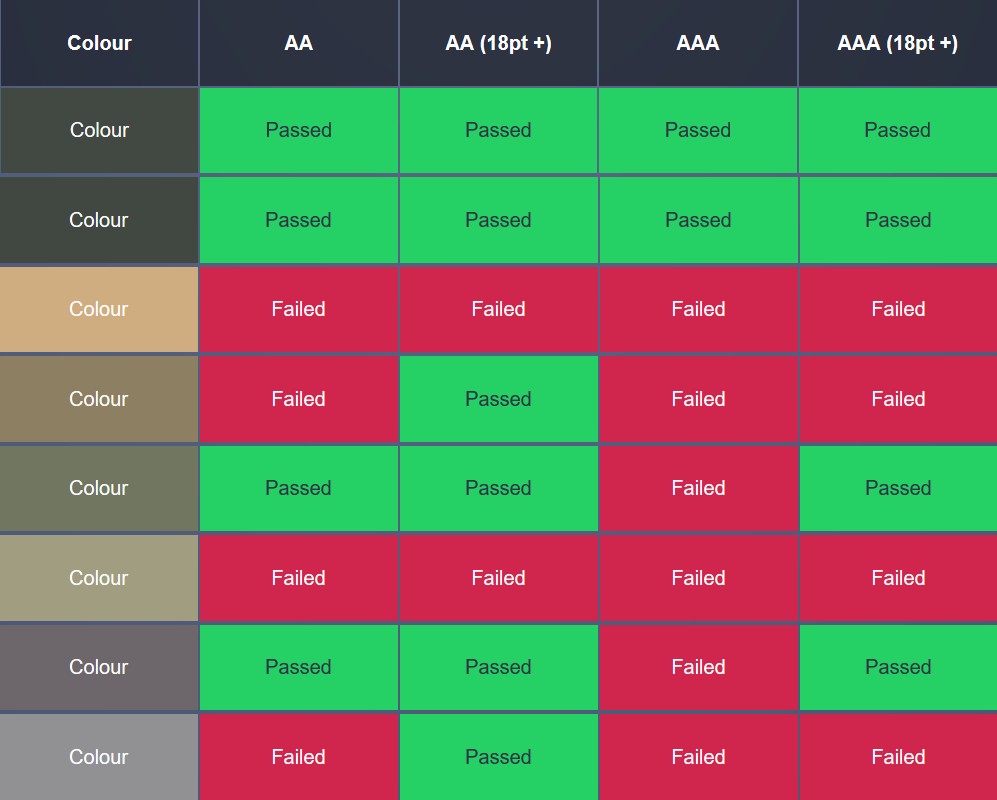
\includegraphics[width=\textwidth]{bjornar/bg-image-eksempel.png}
    \caption{Eksempel}
    \label{fig:analysis-current-a11y_bg-example}
\end{figure}

Vi gjenskapte headeren til Sirkus Media i verktøyet, og testet den store teksten: \q{Vi skaffer konkrete kundehenvendelser} og den mindre teksten \q{Med vår egenutviklede løsning jobber vi for å skaffe våre kunder konkrete kundehenvendelser - direkte på epost og telefon.} Se figur \ref{fig:analysis-current-a11y_bg-generator}. 

\begin{figure}[H]
    \centering
    
\includegraphics[width=\textwidth]{bjornar/bg-image-generator.png}
    \caption{Stor tekst fra header i verktøyet}
    \label{fig:analysis-current-a11y_bg-generator}
\end{figure}

\begin{figure}[H]
    \begin{center}
        \subfigure[Stor tekst]{\label{fig:analysis-current-a11y_bg-h1}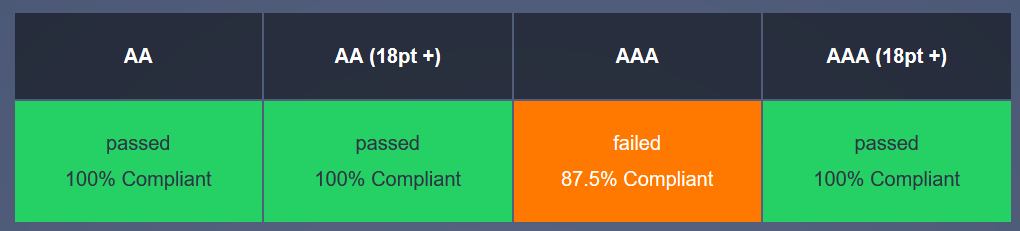
\includegraphics[width=0.475\textwidth]{bjornar/bg-image-h1.png}}
        \subfigure[Liten tekst]{\label{fig:analysis-current-a11y_bg-p}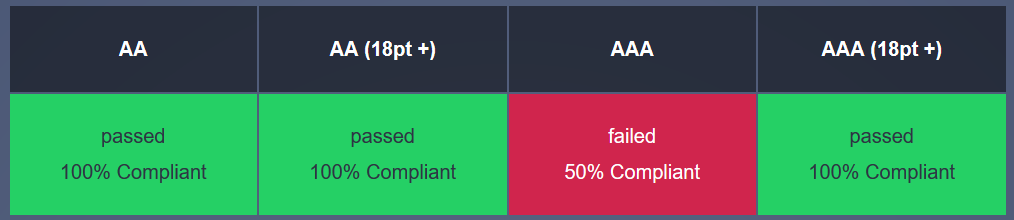
\includegraphics[width=0.475\textwidth]{bjornar/bg-image-p.png}}

        \caption{Testresultat}
        \label{fig:analysis-current-a11y_bg-h1_p}
    \end{center}
\end{figure}

Resultatet som vi ser i figur \ref{fig:analysis-current-a11y_bg-h1_p} viser at teksten i headeren har bra nok kontrastforhold for å passere kravet for AA, men ikke AAA. 

\subsection{Qualys SSL Server Test}
SSL Server Test\footnote{\url{https://www.ssllabs.com/ssltest/}} er en tjeneste som tester SSL og TLS sertifikater. Resultatet på testen ble en A. Dette er bra, men nettstedet burde få et bedre resultatet som A+ eller A++. Det kreves hverken mye tid eller ressurser for å oppnå dette.

\begin{figure}[H]
    \centering
    
\includegraphics[width=\textwidth]{bjornar/ssllabs.png}
    \caption{Sertifikat score}
    \label{fig:analysis-current-ssl}
\end{figure}

\subsection{Test med skjermleser}
Brukervennligheten via skjermleser ble også testet. Nettsiden ble testet med skjermleseren NVDA\footnote{\url{https://www.nvaccess.org/about-nvda/}}. Det var enkelt å navigere seg rundt på nettsiden. Innholdet kom i en logisk rekkefølge og det var lett å navigere seg mellom elementene. Det eneste problemet var kontaktskjema, som er ganske viktig ettersom målet med nettsiden er at potensielle kunder skal ta kontakt. En annen faktor som manglet var en \q{skip to main content}-link.

\subsection{Google Transparency Report - Safe Browsing: malware and phishing}
Til slutt sjekket vi om nettsiden har skadevare på seg med en tjeneste fra Google\footnote{\url{https://transparencyreport.google.com/safe-browsing/search?url=https://sirkusmedia.no&hl=en-US}}. Her ble det ikke gjort noen funn, noe som selvfølgelig er positivt.

\subsection{Konklusjon}
Ut i fra testene gjort med Google Chrome DevTools, Google Lighthouse og Checkbot kan vi konkludere med at nettsiden er rask. På testen gjort ved høgskolen laster siden inn på under 1 sekund i gjennomsnittet, noe som er meget bra. Siden får over 70\% i poengsum fra Google Lighthouse og Checkbot. Med relativt enkle forbedringer, kan vi få denne summen opp til mellom 90-100\%.

Når det kommer til universell utforming gjør Sirkus Media det bra og følger de lover og regler som gjelder i Norge vedrørende dette. Vi ser likevel at kontrastforholdene på siden er gode nok for kravene til nivå AA, men ikke helt for AAA. Dette er noe som kan forbedres.

Totalt sett gjør nettstedet til Sirkus Media det bra på testene som vi kjørte den gjennom. Som tidligere nevnt er hovedgrunnen til dette at dagens nettsted består av kun en forside og lite informasjon. Dette begrenser muligheten for feil. Det vil være en utfordring å gjøre det like bra i disse testene med et nettsted som består av flere sider, mer innhold og kompleks funksjonalitet.

\section{Konkurrentanalyse}

Målet med konkurrentanalysen er å finne inspirasjon til nettstedet vi skal utvikle ved å se på allerede eksisterende løsninger. Hvem er oppdragsgiver sine konkurrenter? Hvordan type løsning har disse valgt? Hvilke styrker og svakheter har løsningene? Analysen er først og fremst gjort av gruppen med vekt på å se det fra en vanlig bruker sitt perspektiv, men noen tekniske faktorer har også blitt vurdert.

\subsection{Teknisk analyse}
For å vurdere de tekniske faktorene har vi brukt Google Lighthouse til å sjekke hvor raskt nettstedene lastes inn, beste praksis og SEO. I tillegg ble WAVE \footnote{Web Accessibility Evulation Tool. http://wave.webaim.org/} brukt til å sjekke om nettstedene følger kravene for loven om universell utforming og tilgjengelighet.

\subsection{Konkurrentene}
Sirkus Media har mange konkurrenter, deriblant alle firmaer som driver mediebyråvirksomhet. Etter samtale med Hans Christian Hymer \footnote{Samtale med oppdragsgiver (16.01.2019)} fikk vi oppgitt 3 bedrifter som blir ansett som Sirkus Media sine største konkurrenter. Det er følgelig disse konkurrentene vi har valgt å analysere.

\subsection{TACTIC™ Real-Time Marketing}
Nettstedet til TACTIC™ Real-Time Marketing ligger på følgende domene; https://tacticrealtime.com. Se figur \ref{fig:competitors-tacticrealtime.com} for bilde av nettstedet.

\subsubsection{Førsteinntrykk}
Førsteinntrykket er at nettstedet fremstår ryddig og profesjonelt. Det første som møter deg er et stort bakgrunnsbilde. Bilde dekker hele skjermen og har en tittel og en underoverskrift. Headeren består også av en knapp der du kan trykke på \q{Request a demo}. Helt øverst på forsiden er logoen til Tactic og en meny. Til høyre er det en knapp som gir deg muligheten til å se på en video. 

\begin{figure}[H]
    \centering
    
\includegraphics[width=\textwidth]{line/tacticrealtime_com_(1366x768).png}
    \caption{tacticrealtime.com}
    \label{fig:competitors-tacticrealtime.com}
\end{figure}

\subsubsection{Forside og undersider}

Forsiden består av bakgrunnsbilde som inneholder logo, meny, overskrifter og en video.  
Deretter kommer det en beskrivende tekst om firmaet, informasjon om plattformen, logo av ledende  Ad-servers og DSP's, partnerprogram og utvalgte kunder. Siden avsluttes med en \q{Contact us}-seksjon.

Nettstedet består også av følgende undersider:
\begin{itemize}
\item Platform
\item Company
\item Partners
\item Clients
\item Blog
\end{itemize}

\subsubsection{Teknisk analyse}

\begin{figure}[H]
    \begin{center}
        \subfigure[Google lighthouse]{
            \label{fig:competitors-lighthouse-summary-tacticrealtime.com}
            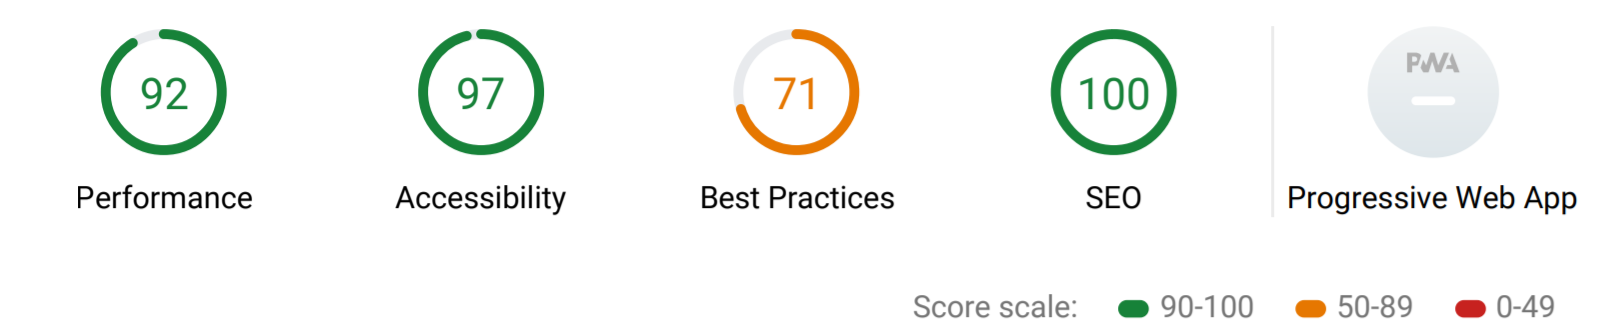
\includegraphics[width=0.7\textwidth]{line/tacticrealtime_com-lighthouse.png}
        }
        \rulesepv
        \subfigure[WAVE]{
            \label{fig:competitors-wave-summary-tacticrealtime.com}
            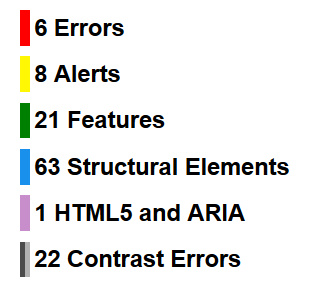
\includegraphics[width=0.2\textwidth]{line/tacticrealtime_com-wave.png}
        }
        
        \label{fig:competitors-tech_analysis-tacticrealtime.com}
        \caption{Resultat fra teknisk analyse av tacticrealtime.com}
    \end{center}
\end{figure}

Etter å ha gjennomført testen til Google Lighthouse, viste det seg at TACTIC var den desidert beste på alle punkter av de 3 konkurrentene. Restultatene fra Google Lighthouse kan man se i figur \ref{fig:competitors-lighthouse-summary-tacticrealtime.com}. Bedriften gjør relativt få feil med tanke på ytelse. Feilene som gjelder \q{Eliminate render-blocking resources}\footnote{Hva vil dette si?} og \q{Serve static assets with an efficient cache policy}\footnote{Hva vil dette si?} burde rettes opp. Vi kan se at siden lastet inn på 2,7 sekunder. Fikser man de overnevnte feilene, vil man kunne mer enn halvere innlastningstiden i følge rapporten.

Når det kommer til \q{Best Pracices}, så er det et par forbedringer TACTIC burde gjort. De burde benytte HTTP2, i stedet for HTTP \footnote{HTTP2 er bakoverkompatibel, så ingen grunn til å ikke bruke det. Samt at det pleier å være 1 linje med kode for å skru på for de fleste web-servere.}. Det linkes også til et JavaScript-bibliotek med kjente sikkerhetshull. Dette burde man på ingen måte gjøre.

På SEO-delen av testen fikk TACTIC 100 av 100 poeng og det er derfor ingenting å påpeke her.

Full rapport for Google Lighthouse kan leses i vedlegg X1.

Figur \ref{fig:competitors-wave-summary-tacticrealtime.com} viser resultatene fra WAVE. Fra resultatene ser man at Tactic fikk 6 feilmeldinger når det kommer til universell utforming. I tillegg har nettsiden deres 22 kontrastfeil. 

\subsubsection{Styrker}
En stor fordel er at nettstedet gir et bra førsteinntrykket. Dette fordi nettstedet fremstår som profesjonelt. Førsteinntrykket er dermed med på å styrke brukerens inntrykk av bedriften. Nettstedet har også god oppbygning og struktur. Løsningen har også en sterk profil, hvor det er ganske tydelig at det er grønn som er primærfargen til selskapet.

\subsubsection{Svakheter}
Noe som kan være en svakhet er at hele nettstedet er på engelsk og i tillegg er på et .com-domene. Disse to faktorene kan forvirre brukerne. En av grunnen til dette er at det er vanskelig å skjønne at dette er et firma som er lokalisert i Oslo. En annen svakhet er at det er lite luft rundt noen elementer, som fører til at nettstedet fremstår som kompakt og mer rotete. Det er heller ikke samme mengde luft over og under elementene. Dette er også med på å trekke ned helhetsinntrykket. Det er heller ikke så lett å bevege seg rundt på nettstedet ved hjelp av tastaturet ettersom TACTIC har fjernet all visuell indikasjon for fokus. Dette gjør at nettsiden ikke oppfyller noe som er et krav i loven om universell utforming og tilgjengelighet. I tillegg får nettstedet mange kontrastfeil, som også bryter lovkravet om universell utforming.

\subsection{Marketer Technologies AS}
Nettstedet til Marketer Technologies AS ligger på følgende domene;
https://marketer.tech/. Se figur \ref{fig:competitors-marketer.tech} for bilde av nettstedet.

\subsubsection{Førsteinntrykk}
Førsteinntrykket av nettstedet er positivt, fordi den fremstår som ryddig og profesjonell. Det første som møter deg er headeren\footnote{Hodet til nettstedet} til nettstedet, som inneholder logoen til firmaet og en meny. Under menyen er en tittel, en underoverskrift og to lenker. Headeren inneholder også et ikon for chat. Det at kunder enkelt kan ta kontakt med firmaet kan virke betryggende, og kan være med å øke troverdigheten til bedriften.

\begin{figure}[H]
    \centering
    
\includegraphics[width=\textwidth]{line/marketer_tech_(1366x768).png}
    \caption{marketer.tech}
    \label{fig:competitors-marketer.tech}
\end{figure}

\subsubsection{Forside og undersider}

Forsiden, i tillegg til headeren, består av logo til noen utvalgre kunder, prosessen til Marketer, animasjoner, resultater fra tidligere prosjekter og en presentasjon av deres løsninger. Helt nederst på siden kommer bunnfeltet, der organisasjonsnummeret, kontaktinformasjon og adresse blir presentert.

Nettstedet består også av følgende undersider:
\begin{itemize}
\item Solutions
\item Company
\item Customers
\item Blog
\item Careers 
\item Contact
\item Book demo
\end{itemize}

\subsubsection{Teknisk analyse}
\begin{figure}[H]
    \begin{center}
        \subfigure[Google lighthouse]{
            \label{fig:competitors-lighthouse-summary-marketer.tech}
            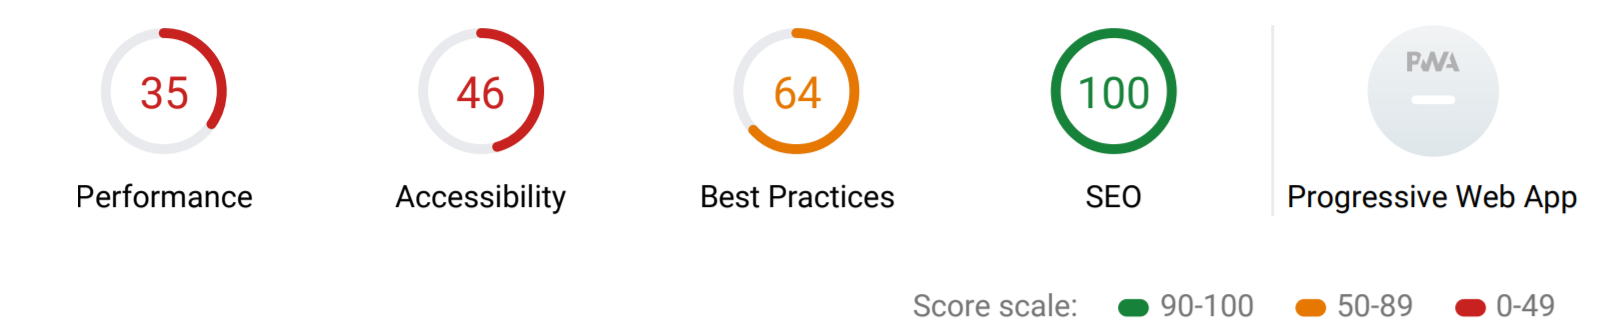
\includegraphics[width=0.7\textwidth]{line/marketer_tech-lighthouse.png}
        }
        \rulesepv
        \subfigure[WAVE]{
            \label{fig:competitors-wave-summary-marketer.tech}
            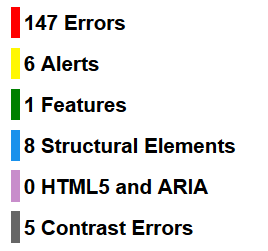
\includegraphics[width=0.2\textwidth]{line/marketer_tech-wave.png}
        }
        
        \label{fig:competitors-tech_analysis-marketer.tech}
        \caption{Resultat for teknisk analyse av marketer.tech}
    \end{center}
\end{figure}

Figur \ref{fig:competitors-lighthouse-summary-marketer.tech} viser resultatene fra testen gjort med Google Lighthouse. Her kom Marketer dårligst ut. Testen påpeker flere feil på punkter vedrørende ytelse, tilgjengelighet og beste praksiser. Det tar Google 5,3 sekunder å laste inn nettstedet, noe som er relativt tregt, men det er raskere enn Inviso.no. Selv om Marketer sin side laster inn raskere, så får den en dårligere poengsum på ytelse. Dette fordi det tar hele 15,2 sekunder før siden blir beregnet som interaktiv \footnote{\q{Time to Interactive} i Google Lightouse rapporten}. Marketer burde ta samme grep som TACTIC, i tillegg til å fjerne ubrukt CSS, servere skalerte bilder og vurdere å redusere antall animasjoner.
Full rapport for Google Lighthouse kan leses i vedlegg X2.

Figur \ref{fig:competitors-wave-summary-marketer.tech} viser WAVE-resultatene. Her kommer det frem at løsningen har 5 kontrastfeil og hele 147 feil når det kommer til universell utforming og tilgjengelighet. 135 av disse feilmeldingene er manglende bruk av alt-tekster.

\subsubsection{Styrker}
En av styrkene er at nettstedet gir et bra førsteinntrykk. Det er også et nettsted som skiller seg ut og er gjennomført. En annen styrke er at løsningen inneholder chat, der kunder enkelt kan ta kontakt. Profilen er også klar og tydelig, og det er åpenbart at bedriften har sort som primærfarge og turkis som aksentfarge.

\subsubsection{Svakheter}
En ulempe er at nettstedet består av flere store filer, som fører til at nettstedet oppleves som tregt. En annen svakhet er at løsningen får mange feil når det kjøres tester på universell utforming og tilgjengelighet. Det er i tillegg vanskelig å navigere seg rundt på nettstedet ved hjelp av kun tastatur.


\subsection{Inviso AS}
Nettstedet til Inviso AS ligger på følgende domene;
https://www.inviso.no/. Se figur \ref{fig:competitors-inviso.no} for bilde av nettstedet.

\subsubsection{Førsteinntrykk}
Førsteinntrykket av nettstedet er at den fremstår som rotete. Hovedgrunnen til dette er at det er mange elementer og mye som skjer i headeren. Logoen og noe av teksten på bakgrunnsbilde er også vanskelig å se på grunn av det dårlige kontrastforholdet. 

\begin{figure}[H]
    \centering
    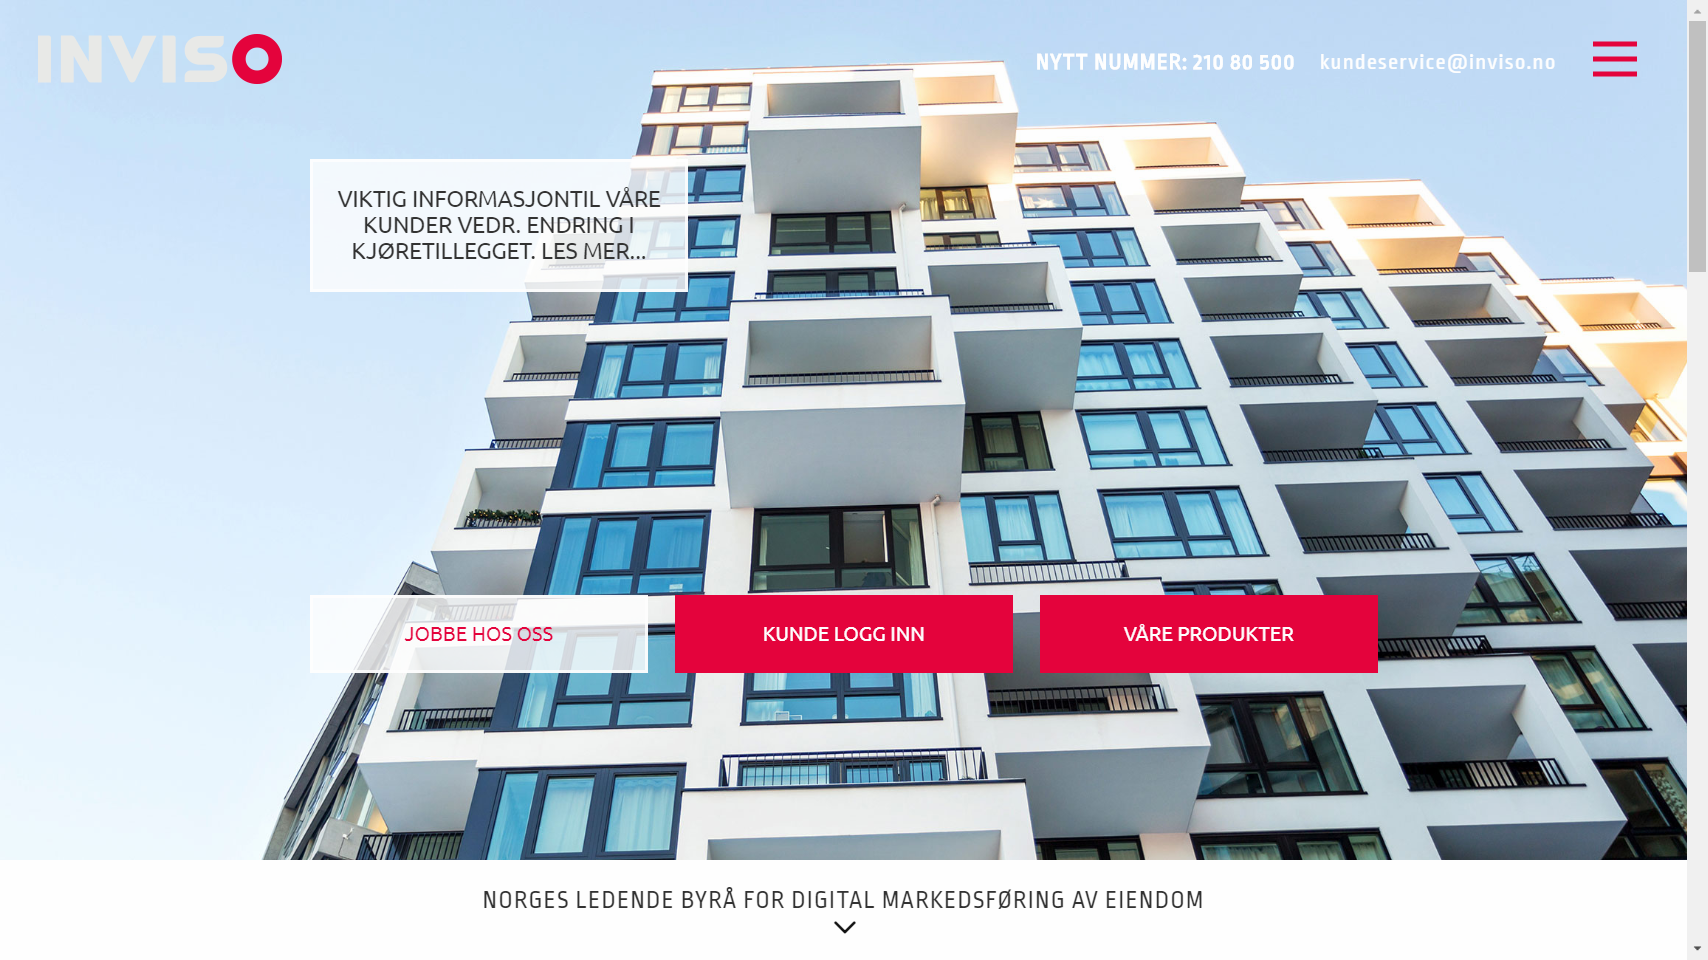
\includegraphics[width=\textwidth]{line/inviso_no_(1366x768).png}
    \caption{inviso.no}
    \label{fig:competitors-inviso.no}
\end{figure}

\subsubsection{Forside og undersider}
I tillegg til headeren består forsiden av \q{Om oss}-tekst, deres tjenester og utvalgte kunder. 

Nettstedet består også av følgende undersider:
\begin{itemize}
\item Inviso
\item Våre produkter
\item Kontakt
\item Galleri
\item Verktøy
\item Nyheter
\end{itemize}


\subsubsection{Teknisk analyse}

\begin{figure}[H]
    \begin{center}
        \subfigure[Google lighthouse]{
            \label{fig:competitors-lighthouse-summary-inviso.no}
            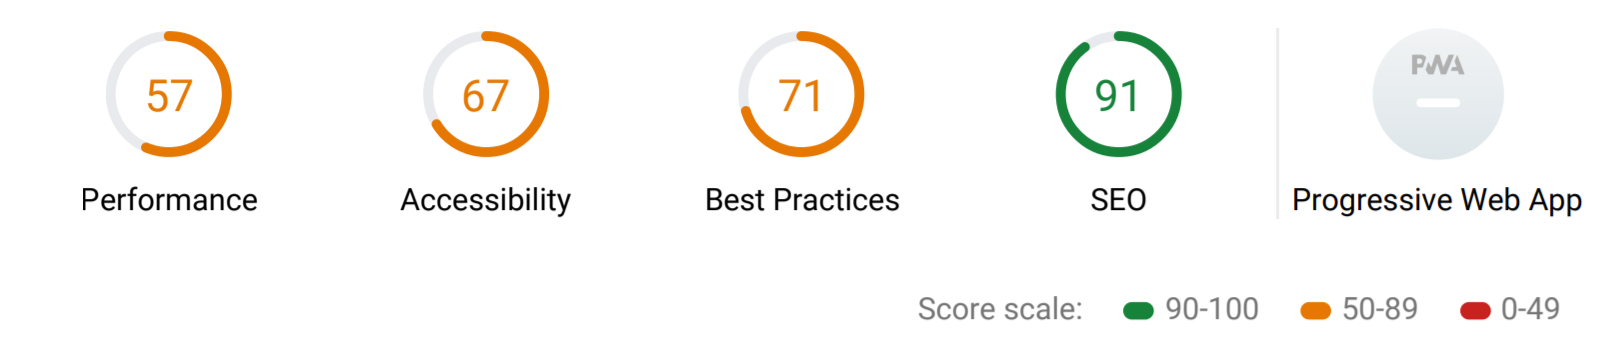
\includegraphics[width=0.7\textwidth]{line/inviso_no-lighthouse.png}
        }
        \rulesepv
        \subfigure[WAVE]{
            \label{fig:competitors-wave-summary-inviso.no}
            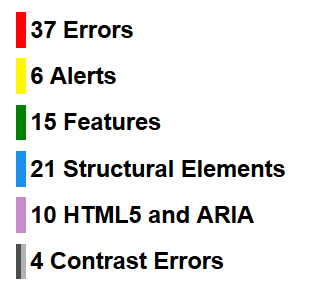
\includegraphics[width=0.2\textwidth]{line/inviso_no-wave.png}
        }
        
        \label{fig:competitors-tech_analysis-inviso.no}
        \caption{Resultat for teknisk analyse av inviso.no}
    \end{center}
\end{figure}

Figur \ref{fig:competitors-lighthouse-summary-inviso.no} viser resultatene fra testen gjort av Google Lighthouse. Her havnet Inviso midt på treet og kom dermed på andreplass av de tre konkurrentene. Bedriften får en helt grei poengsum i gjennomsnitt. Når det kommer til ytelse, bør de ta samme grep som både TACTIC og Marketer. Hovedproblemet her er at bildene serveres i en lite egnet filtype, og kan enkelt løse ved å velge en filtype som er mer egnet. Ved å fikse dette kan de hente inn hele 4,2 sekunder av den totale innlastningstiden på 6,7 sekunder.

På test delen vedrørende tilgjengelighet kommer det frem av Inviso burde forbedre kontrastforhold på deler av siden sin.

Ingenting spesielt å påpeke ved SEO, men Inviso burde absolutt ta en titt på hvilke JavaScript-biblioteker de bruker, ettersom Google kan melde om hele 5 kjente sikkerhetshull er tilgjengelig på siden. Full rapport for Google Lighthouse kan leses i vedlegg X3.

Ved å kjøre test via WAVE oppgir resultatet at nettstedet har 4 kontrastfeil. Nettstedet får også 37 feilmeldinger når det gjelder universell utforming. Figur \ref{fig:competitors-wave-summary-inviso.no} viser resultatene fra WAVE-testen.

\subsubsection{Styrker} 
En av styrkene er at nettstedet har en bra profil. Det er lett å skjønne at rød er primærfargen til Inviso. En annen positiv side er at det tekstlige innholdet på siden er godt skrevet og får bedriften til å fremstå profesjonelt.

\subsubsection{Svakheter}
En svakhet er at det er for mye informasjon i headeren. Dette kan bidra til at førsteinntrykket blir dratt ned. En annen stor svakhet er at nettstedet får mange feil når man kjører tester når det gjelder universell utforming og tilgjengelighet. Det faktum at nettsiden har en mobil-meny på fullversjon av siden, trekker også ned fordi dette gjør brukeropplevelsen dårligere.

\subsection{Konklusjon}
Felles for alle 3 konkurrentene er at ingen av de følger loven om universell utforming og tilgjengelighet. Universell utforming er lovpålagt i Norge \footnote{\url{https://lovdata.no/dokument/SF/forskrift/2013-06-21-732}}, og vår løsning kommer derfor til å følge disse kravene. 

En annen faktor konkurrentene har til felles er at de presenterer sine kunder og/eller partnere. Dette bør også Sirkus Media gjøre. Presentasjon av kundeforhold med kjente firmaer er tillitsvekkende og kan skape bedre troverdighet blant brukerne. \footnote{Kilde?}

Figur \ref{fig:competitors-mobile} viser at alle konkurrentene har gått for samme løsning når det kommer til design på mobil. Alle har bedriftens logo oppe til venstre og et meny ikon til høyre. Undersøkelser \footnote{Kilde: Luke Wroblewski, en internasjonalt anerkjent brukeropplevelsesdesigner \url{https://www.lukew.com/ff/entry.asp?1945}} viser at dette er langt fra den mest optimale løsningen. Planen er derfor at vår løsning skal ha en annen struktur.

Konkurrentene har gode løsninger, men også en del svakheter som har blitt påpekt i denne analysen. Konkurrentanalysen har vært nyttig fordi den både har ført til at gruppen har fått inspirasjon til deler av den løsningen som skal utvikles og samtidig gitt en pekepinn på hva som bør gjøres annerledes.

Studentgruppen har satt som mål å få minst like bra score på testen til Google Lighthouse, som gjennomsnittsscoren til de utvalgte konkurrentene.

\begin{figure}[bh]
    \begin{center}
        
\includegraphics[width=0.3\textwidth]{line/tacticrealtime_com_(iPhone_6_7_8).png}
        
\includegraphics[width=0.3\textwidth]{line/marketer_tech_(iPhone_6_7_8).png}
        
\includegraphics[width=0.3\textwidth]{line/inviso_no_(iPhone_6_7_8).png}
        \caption{Alle nettstedene er mobiltilpasset}
        \label{fig:competitors-mobile}
    \end{center}
\end{figure}




\section{Teknologier}
Når det kommer til utvikling av nettsteder finnes det mange ulike teknologier, systemer og verktøy som kan benyttes for å få det samme resultatet. Derfor er det viktig å kartlegge brukerens behov og deretter sette ønskede kvalifikasjoner og krav, slik at de valgte verktøyene er tilpasset dette. Basert på de foregående analysene i dette kapittelet har studentgruppen kommet frem til et sett med minimumskrav. Videre blir passende verktøy og tilhørende teknologier presentert.

\subsection{Krav til teknologier}
Følgende sett med minimumskrav er satt med basis i den foregående analysen:


\subsection{Designmønster}
\subsection{Verktøy til grafisk design}
\subsection{Verktøy til back-end}
\subsection{Verktøy til front-end}
\subsection{Andre verktøy}
\subsection{Tilhørende teknologier og begreper}
\subsection{Verktøyanalyse}

\subsubsection{Laravel}
Laravel\footnote{\url{https://laravel.com/}} er et PHP-rammeverk, med åpen kildekode, som brukes til å lage webapplikasjoner og andre nettsteder. Rammeverket baserer seg på Symfony\footnote{Avsnitt \ref{sec:tools-symfony}} og følger Model-view-controller\footnote{Avsnitt \ref{sec:tools-mvc}} (MVC) designmønsteret.
Laravel kommer med innebygde funksjoner for autentisering, modeller, visninger, sesjoner, ruting og andre funksjoner som en \textit{templating engine} kalt Blade\footnote{\url{https://laravel.com/docs/5.7/blade}}.

%%% VI SER PÅ FORDELER OG ULEMPER SENERE %%%
%\textbf{Fordeler}
%\begin{itemize}
%    \item Laravel er veldig raskt i forhold til CMS (Content Management Systems).
%    \item Har funksjoner som autentisering og autorisasjon.
%    \item Alt kan tilpasses og styres hvordan tingene fungerer.
%    \item Databasen kan brukes eller utformes på egen måte.
%\end{itemize}

%\textbf{Ulemper}
%\begin{itemize}
%    \item I Laravel må SEO definere egne ruter, og det tar mye arbeid å utvikle et nettsted som hovedsakelig er avhengig av innhold.
%    \item Laravel rammeverk er litt komplisert og krever mer kunnskap.
%    \item Laravel er mindre fleksibel for å oppdatere innholdet.
%\end{itemize}

%Fordeler og Ulemper av laravel ble tatt i forhold til CMS.
%Kilde: \url{https://www.educba.com/laravel-vs-wordpress/}

\subsubsection{Symfony}
\label{sec:tools-symfony}
Symfony er et webapplikasjonsrammeverk og er et sett med gjenbrukbare komponenter og biblioteker skrevet i PHP. \cite{symfony19wis}

\subsubsection{MVC}
\label{sec:tools-mvc}
Model-View-Controller (MVC)\footnote{\url{http://www.dgp.toronto.edu/~dwigdor/teaching/csc2524/2012_F/papers/mvc.pdf}} er et designmønster som deler et program inn i tre hovedkomponenter: modell, visning og kontroll.\cite{burbeck87aps} Oppbygningen kan enkelt forklares ved hjelp av et eksempel fra Matteo publisert på dev.to:
Matteo J. (2018, Mars 16) Re: Explain MVC like I'm five [Blogg kommentar]\footnote{\url{https://dev.to/matteojoliveau/comment/2ikd}}
\begin{quote}
    You walk in a McDonald and you order at the big interactive touchscreen.
    The screen is the View, and you ask for your meal there.
    The order is passed to the operator, who is the Controller, that will go in the kitchen and fetch a burger (your wanted resource) of the type (Model) you asked, then deliver it back to you.
\end{quote}
%Typisk flyt er at det kommer inn en forespørsel som går til kontrolleren. Den tolker forespørselen og behandler den ved å hente og endre data via modell. Til slutt sendes det et svar til visning.

\textbf{Modell} (Model) representerer de forskjellige type ressurser en applikasjon har. Her beskrives hver ressurs, hvordan den er oppbygd og hva som kan gjøres med den.

\textbf{Visning} (View) håndterer brukerinteraksjon og presentasjon av data. Er ofte et grafisk brukergrensesnitt.

\textbf{Kontrolleren} (Control) delen er ansvarlig for å koordinere forespørsler og svar.

\subsubsection{GNU/Linux}
GNU/Linux er en familie med Unix-lignende operativsystemer som baserer seg på Linux-kjernen og en del programvare fra GNU-prosjektet.
I denne familien finner vi blant annet Ubuntu, Debian, Fedora, Red Hat Linux og Arch Linux.
Kilder: \url{https://www.kernel.org} \url{https://www.gnu.org/} \url{https://www.ubuntu.com/} \url{https://www.debian.org/} \url{https://getfedora.org/} \url{https://www.redhat.com/en/topics/linux} \url{https://www.archlinux.org/}

\subsubsection{Nginx}
Nginx er en gratis HTTP-server med åpen kildekode. Nginx har mulighet til å håndtere høy belastning av HTTP-forespørsler. Programmet er tilgjengelig på operativsystemer som Windows, Mac OS og Solaris. I tillegg er Nginx tilgjengelig på operativsystemer som er basert på GNU/Linux eller BSD.

Kilde: Nedelcu, C. (2010). Nginx HTTP Server: Adopt Nginx for Your Web Applications to Make the Most of Your Infrastructure and Serve Pages Faster Than Ever. Packt Publishing Ltd.

\subsubsection{PHP}
PHP (rekursiv akronym for PHP Hypertext Pre-processor) er et skriptspråk som er spesielt egnet for webutvikling og kan legges inn i filer sammen med HTML. PHP er et serverside programmeringsspråk og kan brukes til å lage dynamiske og interaktive nettsteder. PHP er gratis og plattformuavhengig, samtidig som det er  er raskt og fleksibelt. Det kan installeres i pakker med webserver og database. Eksempelvis LAMP, LEMP, WAMP og XAMPP. PHP er også mulig å installere enkeltstående. 

Kilde: \url{http://php.net/}

\subsubsection{Sesjoner}
En sesjon\footnote{\url{https://ieeexplore.ieee.org/abstract/document/8392612}} (session) er en samling av data lagret på en webserver. En webserver tildeler en ID til hver bruker som sender forespørsler via en nettleser. ID-en lagres som en informasjonskapsel i nettlesern til brukeren. Alle nye forespørsel vil så identifiseres av ID-en som er lagret hos brukeren.

\subsubsection{phpMyAdmin}
phpMyAdmin\footnote{\url{https://www.phpmyadmin.net/}} er et gratis og webbasert administrasjonsverktøy for MySQL og MariaDB databaser. Verktøyet er skrevet i PHP og JavaScript. Med phpMyAdmin kan man lage, endre og slette databaser, tabeller og felter. Annen funksjonalitet kan være å utføre SQL-setninger, administrere nøkler og privilegier og eksportere data til ulike formater.

\subsubsection{MariaDB}
MariaDB er et relasjonsdatabasesystem basert på MySQL, som er gratis og har åpen kildekode. Systemet funker som en \textit{drop-in} erstatning for MySQL.

Kilde \url{https://mariadb.org/}

\subsubsection{CSRF}
Cross site request forgery\footnote{\url{https://ieeexplore.ieee.org/abstract/document/5283085}} (CSRF) er angrep som tvinger brukere til å utføre uønskede handlinger på en nettside der brukeren er logget inn, via en annen nettside. For eksempel: hvis brukeren er logget inn på Facebook.com, og går til Twitter.com. Da kan Twitter laste inn et bilde som dette: \lstinline{<img src="https://facebook.com/delete-my-account">}. Dette vil da sende en forespørsel til den linken, som kan føre til sletting av konto. Om Facebook ikke har implementert mottiltak for slike angrep, vil denne forespørselen tolkes som om den kommer direkte fra brukeren.

\subsubsection{CI \& CD}
CI står for continuous integration og CD står for continuous delivery. CI/CD\footnote{\url{https://www.atlassian.com/continuous-delivery/principles/continuous-integration-vs-delivery-vs-deployment}} er en metode som lar utviklere implementere og levere kodeendringer raskt og pålitelig.

\subsubsection{Buddy}
Buddy\footnote{\url{https://buddy.works}} er en webbasert applikasjon for CI og CD. Applikasjonen lar utviklere bygge, teste og distribuere nettsider og programkode automatisk når kildekoden oppdateres. For eksempel er det mulig å koble Buddy til et nettsteds kildekode via Git. Når koden til nettstedet oppdateres, vil Buddy automatisk detektere endringer og starte en byggeprosess. Når byggeprosessen er ferdig kjøres det automatisk tester på koden, som verifiserer at alt fungerer. Deretter vil Buddy laste koden opp til en server og oppdatere nettstedet som ligger ute på nett. Dette skjer gjerne gjennom Docker\footnote{\url{https://www.docker.com/}} sammen med Kubernetes\footnote{\url{https://kubernetes.io/}}.

\subsubsection{Axios}
Axios\footnote{\url{https://github.com/axios/axios}} et et JavaScript-bibliotek for en promise-basert\footnote{\url{https://leanpub.com/exploring-es6/}} HTTP-klient som kan kjøres i nettlesere og Node.Js. Biblioteket gjør det enklere å lage og behandle asynkrone forespørsler.

\subsubsection{Git}
Git er et system for versjonskontroll. Et versjonskontrollsystem blir hovedsaklig brukt under utvikling av software og nettsteder. Det kan også brukes til andre type prosjekter som grafisk design og skriving av dokumenter.

Ved å bruke Git opprettes det historikk over alle endringer, samt en sikkerhetskopi av alle versjoner av filene.

En annen fordel ved å bruke Git er at det blir enklere å samarbeide med andre, uten å måtte tenke på at alle må sitte på nyeste versjon av filene.

KILDE (GIT OG GITHUB): \url{https://journals.plos.org/ploscompbiol/article?id=10.1371/journal.pcbi.1004668}
\url{https://searchitoperations.techtarget.com/definition/GitHub}

\subsubsection{Github}
GitHub.com er et nettsted for å hoste git repositories, og blir mye brukt for \q{Open Source}-prosjekter. 

Github er et sentralisert punkt for å samle en brukers repositories. Ved siden av å hoste repositories, lar GitHub brukere dele repositories med hverandre, lage informasjonssider om prosjektet og opprette saker (issues).
 
\subsubsection{Overleaf}
Overleaf\footnote{\url{http://web.simmons.edu/~wilsonjd/LIS488/website/OverleafTutorial.pdf}} er en tjeneste som brukes til å lage, redigere og dele akademiske artikler på nettet ved hjelp av LaTeX. Dette er et nettbasert tekstforfattings-program. 
Overleaf v2\footnote{\url{https://no.overleaf.com/learn/how-to/Working_Offline_in_Overleaf}} tilbyr synkronisering med GitHub og Dropbox.

\subsubsection{Ottomatik.io}
Ottomatik\footnote{\url{https://ottomatik.io/}} er en webbasert tjeneste for automatisk sikkerhetskopiering av filer og MySQL databaser.

\subsubsection{Amazon S3}
Amazon Simple Storage Service\footnote{\url{https://aws.amazon.com/s3/}} er en webbasert tjeneste som tilbyr objekt-lagring. Tjenesten tilbyr meget god skalerbarhet, datatilgjengelighet, sikkerhet og ytelse.

KILDE: https://dash.harvard.edu/handle/1/24829568

\subsubsection{HTTP/2}
HTTP/2\footnote{\url{https://www.rfc-editor.org/rfc/pdfrfc/rfc7540.txt.pdf}} er en revisjon av HTTP-nettverksprotokollen. HTTP er et sett med regler for overføring av filer (tekst, grafiske bilder, lyd, video og andre mediefiler). Et av de store målene med HTTP/2 var å tillate multipleksing.

\subsubsection{HTTPS}
HTTPS\footnote{\url{https://www.rfc-editor.org/rfc/pdfrfc/rfc2616.txt.pdf}} (Hypertext Transfer Protocol Secure) er en sikker versjon av HTTP-protokollen som overfører data på nett. HTTPS-protokollen krever at det opprettes en kryptert kanal mellom nettleseren og webserveren, slik at overføring mellom disse blir sikker.

\subsubsection{TLS}
Transport Layer Security er en kryptografisk protokoll. Dette er viktig for å sikre informasjon som overføres gjennom nettverk. TLS brukes i forskjellige tjenester som HTTPS, FTPS, VoIP og VPN.
Når en tjeneste bruker en sikker tilkobling, legges bokstaven S til tjenestens protokollnavn. For eksempel: HTTPS, SMTPS, FTPS, SHIPS.
SSL (Secure Socket Layer) er en utdatert forgjenger til TLS.

KILDE: Thomas, S. (2000). SSL and TLS essentials. New Yourk, 3.

\subsubsection{Let’s Encrypt}
Let’s Encrypt\footnote{\url{https://letsencrypt.org/}} er en gratis og åpen sertifikatautoritet som gir ut X.509-sertifikater for kryptering av transportlaget. Tjenesten leveres av ISRG (Internet Security Research Group).

\subsubsection{HTML}
Hypertext Markup Language\footnote{\url{https://www.w3.org/standards/webdesign/htmlcss}} er et markeringsspråk som brukes til å lage nettsidedokumenter. Det er et system som identifiserer og beskriver de forskjellige komponentene i et dokument som overskrifter, avsnitt og lister. HTML5 er den nyeste versjonen av HTML-standarden.

\subsubsection{CSS}
Casecading Style Sheet\footnote{https://www.w3.org/standards/webdesign/htmlcss} er et format for stilsett som beskriver utseendet i en applikasjon eller på et nettsted. CSS styrer blant annet fonter, farger, bakgrunnsbilder, linjeavstand og sidelayout. Formatet lar utviklere style innhold på en slik måte at brukere enklere kan identifisere hva det er, samt være i tråd med en bedrift eller person sin identitet.

\subsubsection{SASS}
Syntactically Awesome Style Sheets\footnote{\url{https://sass-lang.com/}} er en utvidelse av CSS. SASS gir mulighet til å bruke variabler, nestede regler, inline-import og mixins. Alt dette gjør det enklere å gjenbruke CSS syntaks. Med SASS er det mulig å lage stilark raskere. SASS er kompatibel med alle versjoner av CSS. Det er ingen nettlesere som kjører SASS, man må derfor kompilere SASS til CSS for å kunne bruke det på nettsider.

KILDE: Cederholm, D. (2013). Sass for web designers. A Book Apart.

\subsubsection{JavaScript}
JavaScript\url{https://developer.mozilla.org/en-US/docs/Web/JavaScript} er et programmeringsspråk som følger ECMAScript-spesifikasjonen. Det er mye brukt til å utvikle webapplikasjoner. Språket støttes av de fleste moderne nettlesere, og brukes til å manipulere elementene på nettsiden og stilene som er brukt på dem. JavaScript støtter objektorientert- og funksjonell programmering.

\subsubsection{React}
React\footnote{\url{https://reactjs.org/}} er et fleksibelt JavaScript-bibliotek for å bygge brukergrensesnitt, og brukes som visningslaget for webapplikasjoner som følger MVC. React har åpen kildekode og er utviklet av Facebook.

Alternativ kilde: \url{https://www.fullstackreact.com/assets/media/sGEMe/MNzue/30-days-of-react-ebook-fullstackio.pdf}

\subsubsection{REST-API}
Et API (programmeringsgrensesnitt) er et sett med funksjoner, prosedyrer, metoder eller klasser som brukes av dataprogrammer for å be om tjenester fra operativsystemet eller programvare som er på datamaskinen. En programmerer kan bruke API-er til å lage applikasjoner.

REST (Representational State Transfer) er en arkitektonisk stil for programvare. Et REST-API er et API som følger REST-stilen og de begrensninger som REST definerer.

KILDE: Masse, M. (2011). REST API Design Rulebook: Designing Consistent RESTful Web Service Interfaces. " O'Reilly Media, Inc.".
side 5 og 6

\subsubsection{NODE.JS ?????}

\subsubsection{Figma}
Figma\footnote{\url{https://www.figma.com/}} er et webbasert designverktøy som åpner muligheten for å samarbeide i sanntid. Med Figma er det også mulig å designe mockups og prototyper av applikasjoner og nettsider.

ekstra kilde: \url{https://www.xfive.co/blog/figma-best-designer-developer-cooperation/}

\subsubsection{Google Analytics}
\label{sec:google-analytics}
Google Analytics\footnote{\url{https://analytics.google.com/analytics/web/}} er en gratis, webbasert tjeneste som gir statistikk og grunnleggende verktøy for analyse av bruksdata, søkemotoroptimalisering og markedsføring.

\subsubsection{Google Lighthouse}
Google Lighthouse\footnote{\url{https://developers.google.com/web/tools/lighthouse/}} er et gratis verktøy for å sjekke kvaliteten på nettsider. Det analyserer nettsidens tilgjengelighet, hastighet og SEO, samt om nettsiden følger de beste praksiser både generelt sett og for progressive webapplikasjoner. Lighthouse kan kjøres via Google Chrome DevTools, en nettleserutvidelse i Google Chrome eller via nettsiden \url{https://web.dev/}.

\subsubsection{WAVE}
Web Accessibility Evaluation Tool\footnote{\url{https://wave.webaim.org/about}} er et verktøy som tester universell utforming hos nettsider og hvorvidt de følger visse punkter i WCAG 2.1-standarden og Section 508. Verktøyet er tilgjenglig som en nettleserutvidelse og som en webbasert tjeneste hos \url{https://wave.webaim.org/}.

\section{Testing}

\subsection{Funksjonell testing}
Funker nettstedet slik som Sirkus Media vil?

\subsection{Ikke funksjonell testing}
Funker nettstedet bra, teknisk sett?

\subsection{Brukertesting}
Hva syns brukere om nettstedet?






\section{Akademiske og tekniske dokumenter}

Akademiske og tekniske dokumenter ser noe forskjellige ut avhengig av fagfeltet. Likevel, en litt grundigere analyse avslører en felles hovedstruktur, som egentlig er ganske intuitiv\dots og omtrent lik den vi lærte på barneskolen: {\em Hode, kropp og hale}. Hver av disse hoveddelene består som regel av omtrent de samme elementene. 



\subsection{Mayfield Handbook of Technical \& Scientific Writing}
\label{sec:mayfield}

I følge engelsk terminologi deler man gjerne et dokument opp i {\em Front matter, Body og End (Back) matter}, og det gjøres konsekvent i
Mayfield Handbook of Technical \& Scientific Writing \cite{perelman97mht}. Denne utmerkede kilden finnes også på 
elektronisk form\footnote{\url{http://www.mhhe.com/mayfieldpub/tsw/home.htm}}. 
I kapittelet 
{\em Elements of Technical Documents}\footnote{\url{http://www.mhhe.com/mayfieldpub/tsw/elemtech.htm}}
blir den følgende generiske strukturen foreslått:

\begin{compactitem}
\item Front Matter
\begin{compactitem}
\item Title page
\item Abstract
\item Table of contents
\item List of figures
\item List of tables
\item List of terms
\item Acknowledgments
\end{compactitem}

\item Body
\begin{compactitem}
\item Introduction
\item Background
\item Theory
\item Design criteria
\item Materials and apparatus
\item Procedure
\item Workplan
\item Results
\item Discussion
\item Conclusion
\item Recommendations
\end{compactitem}

\item End Matter
\begin{compactitem}
\item References
\item Appendixes
\item Index
\end{compactitem}

\end{compactitem}

Hvert av punktene blir nærmere beskrevet, med mange eksempler på godt (og dårlig) innhold, og det anbefales på det sterkeste å  studere dette kapitellet nærmere. 

Denne strukturen er så nær man kommer en universell mal for en teknisk/vitenskapelig rapport.

\subsection{HiØ/IT}
\label{sec:hiof-it}

Ved HiØ/IT har man valgt å skille grovt sett mellom to typer dokumentasjon.
{\em Prosessdokumentasjonen} omfatter en forprosjektrapport samt individuelle refleksjonsnotater, og selve produktet er omtalt i
{\em hoveddokumentet}\footnote{\url{https://wiki.hiof.no/index.php/Bacheloroppgaven_-_Leveranser}}(eller rett og slett det vi kaller bacheloroppgaven).
Når det gjelder oppbygging og innhold er hoveddokumentet å regne som en typisk akademisk/teknisk rapport/artikkel:

\begin{compactitem}
\item Tittelside
\item Sammendrag
\item (Takk til)
\item Innholdsfortegnelse
\item (Liste over figurer)
\item (Liste over tabeller)
\item Introduksjon
\item Analyse
\item Design
\item Implementasjon
\item Evaluering
\item Diskusjon
\item Konklusjon
\item Referanser
\item Referanser
\end{compactitem}

\section{Skriveverktøy for store og komplekse dokumenter}

For å starte på et stort og komplekst dokument, vil mange åpne sin vanlige teksteditor og sette igang. Det går sjelden bra. Som ved alle typer større oppgaver, bør man velge sine verktøy med omhu.
Før man setter igang å lage et digitalt dokument, kan det være fornuftig å dvele litt ved hvordan dokumenter har blitt, og blir, produsert på tradisjonelt vis. 

\subsection{Forfatter, redaktør, typograf, trykkeri}

Tradisjonelt hersker det en streng arbeidsdeling innen produksjon av dokumenter, som f.eks. en bok, eller en avis. Forfatteren (eller journalisten) skriver såkalt {\rm brødtekst}, som rett og slett er tekst, skrevet for hånd, på skrivemaskin, eller talt inn på diktafon. I teksten er det gjerne markert ulike strukturelle elementer. Det er markert hvor et nytt avsnitt begynner, kanskje det står skrevet at her kommer det en illustrasjon, etc. Dette råmaterialet går gjerne til en redaktør, som kvalitetssikrer innholdet og tildels struktur, og eventuelt foreslår/foretar endringer. Deretter tar typografen (eller den grafiske formgiveren) over, og bestemmer skriftstørrelser, fonter, marger, linjeavstand etc. Til slutt går trykkoriginalen til trykkeriet\footnote{Her kan jo være på sine plass å tenke litt på XHTML og CSS, og hvor de har sine røtter\dots og da tenker jeg ikke på Håkon Wium Lie \smiley.}.

Denne framgangsmåten ivaretar en klar tredeling av arbeidet; innhold, struktur, og form. Innholdet, og grovstrukturen, bestemmes av forfatteren. Redaktøren sørger for å kvalitetssikre innholdet, og eventuelle justere strukturen. Den endelig formgivingen av dokumentet blir typografens rolle. Det er viktig å merke seg at alle disse tre rollene krever høy kompetanse innen helt forskjellige fagfelt. De fleste mener også at det er ganske unaturlig for en forfatter å legge ned mye tankearbeid i hvilken font og størrelse det bør være på overskriftene. På den annen side ville vel det ikke være rett at typografen blandet seg bort i innholdet.

\subsection{The curse of the cursor \\  \normalsize -eller- \\DTP: DeskTop Publishing eller Dom Tokigas Paradis? }

Og etterhvert kom datamaskinene, som tilsynelatende kunne gjøre ``alt'', og dermed begynte mange å gjøre ``alt'', selv. Teksteditorer og desktop publishing verktøy gjorde det mulig for at en person kunne stå for hele prosessen, både skrive, redigere, og formgi, uten å ha særlig kompetanse, ferdighet eller erfaring i noen av feltene.

Personlig husker jeg godt mitt første møte med DTP, tidlig i IT-utdannelsen. Oppgaven var å lage en liten avis, med bilder og det hele, ved hjelp av en søt liten Mac, som på et mysteriøst vis var knyttet sammen med en skriver som til og med skrev ut illustrasjoner og fotografier i grov oppløsning. Den blinkende markøren i teksteditoren var hypnotisk, halvt innbydende, halvt skremmende. Og så måtte man bare kaste seg ut i det. Skrive noen setninger, markere en del som ``bold'' og fontstørrelse 18, fin overskrift, et par ``enter'', forsette med vanlig font, nei, kanskje en litt mer fancy kalligrafifont, kanskje til og med blå? Og dermed var det gjort, forvirringen var total. Noe senere erfarte jeg at i enkelte svenske miljøer mente man at DTP sto for ``Dom Tokigas Paradis". Innen visse segmenter av reklamebransjen mener jeg fremdeles å se spor etter slike traumatiske møter med datastøttet publisering.

Man kan jo spørre seg om det egentlig er noen forskjell mellom et blankt ark, enten på et skrivebord eller i en skrivemaskin, og en blinkende markør øverst i venstre hjørne i en editor? Uansett svar, det blanke arket gir deg ikke anledning til å eksperimentere med fonter, marger, skriftstørrelse og plassering av bilder. Arket handler kun om innhold, og hvordan det skal struktureres, hvilken passasje som følger en annen, og hvor det begynner et nytt avsnitt.

\subsection{Programmering av dokumenter}

Et par år senere skal jeg produsere min første akademiske artikkel, i \LaTeX~med  AMS stilen. Hæh?

Det tok et par dager før jeg skjønte poenget. Skrive innholdet i filer (ark) i en editor uten formateringsmulighet, sette inn kryptiske kommandoer for å markere avsnitt eller matematiske uttrykk, sette sammen delene i en styrefil, legge til noen kommandoer som avgjorde hvordan dokumentet ble seendes ut. Deretter {\em kompilere} hele greia! Som så resulterte i  en DVI-fil\footnote{DVI: DeVice Independent}, som igjen kunne konverteres til alle mulige trykk- og printbare formater. Og det beste av alt, resultatet, rent formmessig, ble helt strøkent, akkurat som i lærebøkene og artikkelsamlingene.

Dette var jo akkurat som å programmere. Full kontroll.


\section{Digital dokumentproduksjon}

Vi foreslår et sett med minimumskrav til digitale dokumentverktøy, basert på  den forutgående analysen. Deretter gir vi kort beskrivelse av 
\LaTeX~ og OpenOffice Writer, som etter en kort vurdering er de to verktøyene som tilfredstiller de fleste av kravene.

\subsection{Generelle krav}
\label{sec:generelle-krav}

Kravene er utarbeidet delvis med basis i den forutgående analysen, men i hovedsak ut fra forfatterens erfaringer.

\vspace{1em}
\begin{compactdesc}
\item [Plattformuavhengighet] I et prosjekt med flere deltagere, er det direkte arrogant å forvente at alle skal bruke samme plattform, fordi valget av dokumentasjonsverktøy krever dette.
\item [Robusthet] En hovedrapport er ofte relativt stor, og tildels med komplekst innhold (figurer, tabeller etc). Det er ikke uvanlig at selv kostbare og vidt utbredte verktøy kræsjer i en slik kontekst, eller verre, begynner å oppføre seg inkonsistent og uforutsigbart Det å åpne et dokument, bare for å oppleve at formatering som ble foretatt kvelden før er ødelagt, er ingen særlig givende erfaring, særlig ikke hvis det er to timer til rapporten skal leveres inn.
\item [Maler/stiler] Det må kunne være mulig å skifte mal på et og samme dokument uten å gjøre ekstra tilpasninger. Dermed oppnår man et klart skille mellom innhold og utforming. Hvis f.eks. retningslinjene for hovedrapporten endrer seg, så er det bare å lage en ny mal og bruke denne.
\item [Oppsplitting]Det bør kunne være mulig å splitte dokumentet i mindre deler, f.eks. en fil for hvert kapittel. Delene må kunne knyttes sammen i et masterdokument. På denne måten vil det være lett å endre rekkefølgen på komponentene. Da er også strukturen uavhengig av det faktiske innholdet. Oppsplitting er også en forutsetning for å kunne jobbe distribuert, der de ulike deltagerne jobber parallelt på ulike deler av rapporten.
\item [Kryssreferanser]Det må være mulig å bruke dynamiske kryssreferanser, slik at man f.eks. kan referere til en nummerert figur. Hvis da nummeret til figuren endrer seg pga. av at det blir lagt inn en figur tidligere i dokumentet, så må referanse oppdateres automatisk.
\item [Bibliografi]De må være enkelt å referere til en ekstern samling bibliografiske referanser. Det også være enkelt å når som helst endre referansestil (f.eks. IEEE eller Harvard).
\item [Brukermasse]Det bør eksistere en stor og variert brukermasse, noe som i seg selv kan være en antydning om at verktøyet holder mål.
\item [Dokumentasjon]Verktøyet må være godt dokumentert, både den innebyggede dokumentasjonen, samt i ulike fora på nettet.
\item [Versjonskontroll]Det må være enkelt å håndtere versjonering, dvs. at man lett kan rekonstruere tidlige versjoner, og lett se hva som er endret fra versjon til versjon.
\item [Framtids/fortidssikker]Verktøyet bør kunne uten videre behandle dokumenter som er laget i tidligere versjoner. Dette vil også være en indikasjon på at dokumentet du jobber fremdeles ``lever'' i rimelig overskuelig framtid. 
\item [Stave/grammatikkontroll] Minimumskravet er at det er mulig å utføre effektiv stavekontroll, for ulike språk, ikke minst norsk bokmål. I tillegg vil det være et pluss om det er mulig å verifisere grammatikk.
\end{compactdesc}


\subsection{\LaTeX}

Klipt og limt fra Wikipedia\footnote{\url{http://no.wikipedia.org/wiki/LaTeX}}:

\begin{quotation}
\LaTeX~ er et typesettingssystem for dokumentproduksjon. Det skrives normalt LaTeX i dokumenter som ikke har hevet og senket tekst.
\LaTeX~ ble opprinnelig utviklet av Leslie Lamport i 1984 og tilbyr idag en lang rekke dokumentproduksjonspakker som f.eks. automatisk opprettelse av innholdsfortegnelser, lister med tabeller og figurer, inkludering av bilder, kryssreferanser, sideoppsett, bibliografier mm.


LaTeX~ baserer seg på at forfatteren av et dokument kun skal være forfatter av dokumentet og slippe å bry seg om utforming og hvordan ting ser ut; noe han normalt sett ikke er ekspert på uansett. Det forfatteren gjør er å dele opp dokumentet i logiske strukturer før han lar LaTeX~ ta seg av selve oppsettet. LaTeX~ ansees ofte som WYSIWYM (det du ser er det du mener) fremfor WYSIWYG (det du ser er det du får) editor. Dette fører til at det ofte anerkjennes som overlegent fremfor andre skriveprogrammer grunnet at endringer som påvirker hele dokumentet er meget enkle å gjennomføre. De trenger ofte bare en endring et sted, så er endringen gjennomført i hele dokumentet.
\end{quotation}


\subsection{OpenOffice Writer (med kloner)}

Klipt og limt fra Wikipedia\footnote{\url{http://no.wikipedia.org/wiki/OpenOffice}}:

\begin{quotation}
Apache OpenOffice (AOO), er en kontorprogramvare som inneholder tekstbehandlingsprogram, regneark, presentasjonsprogram, tegneprogram og et databaseprogram. AOO er fri programvare, og distribueres av Apache Software Foundation under Apache-lisensen. Det betyr at både programmet og dets kildekode kan lastes ned gratis, og privatpersoner eller bedrifter kan selv gjøre endringer eller reparere feil. 

AOO benytter ODF som sitt primære dokumentformat. Dette er en ISO-standard som blant annet er tatt i bruk av offentlig sektor i Norge og EU for utveksling av digitale dokumenter. I tillegg støttes formatene til Microsoft Office og en rekke andre kontorprogrammer. AOO er multiplattform programvare, tilgjengelig for mange forskjellige operativsystemer, deriblant Microsoft Windows, Mac OS X, Linux, Solaris, FreeBSD, NetBSD og OpenBSD.
\end{quotation}


    \cleardoublepage
\chapter{Planlegging av produktet}
\label{chap:design} 

I dette kapittelet tar vi for oss hvordan vi har tenkt å utforme nettstedet. Vi vil presentere forslag til innhold, struktur, design, utforming av CMS og databaser. Dette vil være grunnlaget for resten av oppgaven.

\section{Planlegging av struktur og innhold}
\label{sec:planning-website}

Etter analysen gjort i kapittel \ref{chap:analysis} har studentgruppen kommet frem til at struktur og innhold burde være som følgende: 

\textbf{Forside} Tanken er at hele nettstedet i hovedsak skal bestå av en lang forside. Da dette ikke er beste praksis for søkemotoroptimalisering, vil vi forbedre SEO ved å lenke til andre sider som er mer detaljert. Høyt oppe på siden skal det være en knapp til et kontaktskjema. Telefonnummeret til bedriften skal også være lett tilgjengelig. I tillegg skal forsiden bestå av en beskrivelse av bedriften, presentasjon av hva de tilbyr og steg for steg om prosessen. Videre skal nettstedet ha et kart som er integrert med Google Maps og viser lokasjonen til bedriften. Nederst på nettstedet skal organisasjonsnummer, link til personvern og logg inn til CMS-et bli presentert.

\textbf{Meny} Nettstedets meny skal være tilgjengelig uavhengig av hvilken side brukeren står på. Her skal alltid forside, om oss og kontakt oss være tilgjengelig. 

\textbf{Om oss} Det vil bli opprettet en egen \q{Om oss}-side som er tilgjengelig via menypunktet \q{Om oss}. Denne siden inneholder en mer detaljert presentasjon av Sirkus Media og deres visjon.

\textbf{Kontakt oss} Nettstedet vil i tillegg til kontaktskjema på forsiden, bestå av en egen side med kontaktinformasjon. Her presenteres også relevant informasjon som bedriftens adresse, e-post, mobilnummer og kart. Vi lager en dedikert side for kontaktinformasjon fordi det er positivt med tanke på søkemotoroptimalisering. For eksempel: Hvis en bruker søker på Google etter Sirkus Media og det ikke er en egen side for kontakt oss, vil brukeren kun få treff på forsiden og undersidene som inneholder irrelevant temaer. Siden brukeren ønsker å kontakte Sirkus Media, er det mer brukervennlig å ha en link til kontakt-siden i Google.

\textbf{Logg inn} Dette er en egen side der de ansatte kan logge inn for å komme til brukergrensesnittet for oppdatering og endring av innhold.

\textbf{Administrasjonsside}  På administrasjonssiden kan de ansatte endre og legge til innhold gjennom et brukergrensesnitt.

\textbf{Informasjon om personvern og informasjonskapsler} Personvernsiden skal inneholde en personvernserklæring. Denne forteller hvordan Sirkus Media samler inn og bruker personopplysninger. Målet er å gi brukerne overordnet informasjon om oppdragsgivers behandling av personopplysninger. I tillegg skal den fortelle brukerne hvilke informasjonskapsler som blir brukt på nettstedet.

\textbf{Annet} Alle sidene skal ha tilgang til en chat, der det er mulig å ta direkte kontakt med bedriften.

\section{Definering av CMS}
\label{sec-planning-cms}
Etter å ha planlagt innholdet måtte gruppen sette seg ned og bestemme hvordan systemet skulle fungere. I felleskap kom vi frem til følgende:

\begin{itemize}
    \item CMS-et skal bestå av flere sider (pages).
    \item Hver side inneholder en eller flere komponenter (components), som er gjenbrukbare biter av kode, og kan tilhøre flere sider.
    \item Hver komponent inneholder felter (fields), som holder på innholdet som vises på siden. Det er forskjellige type felter, for eksempel kan et felt være et bilde, et tekstområde eller en lenke. 
\end{itemize}

Videre ble det bestemt at studentgruppen, eller en fremtidig superadmin, ferdigdefinerer komponenter og felter. I brukergrensesnittet til back-end vil oppdragsgiver få mulighet til å opprette sider med ønskede komponenter og felter.  

\section{UML-diagram}
Figur \ref{fig:database} viser databasen som ble planlagt for prosjektet:
\begin{figure}[H]
    \centering
    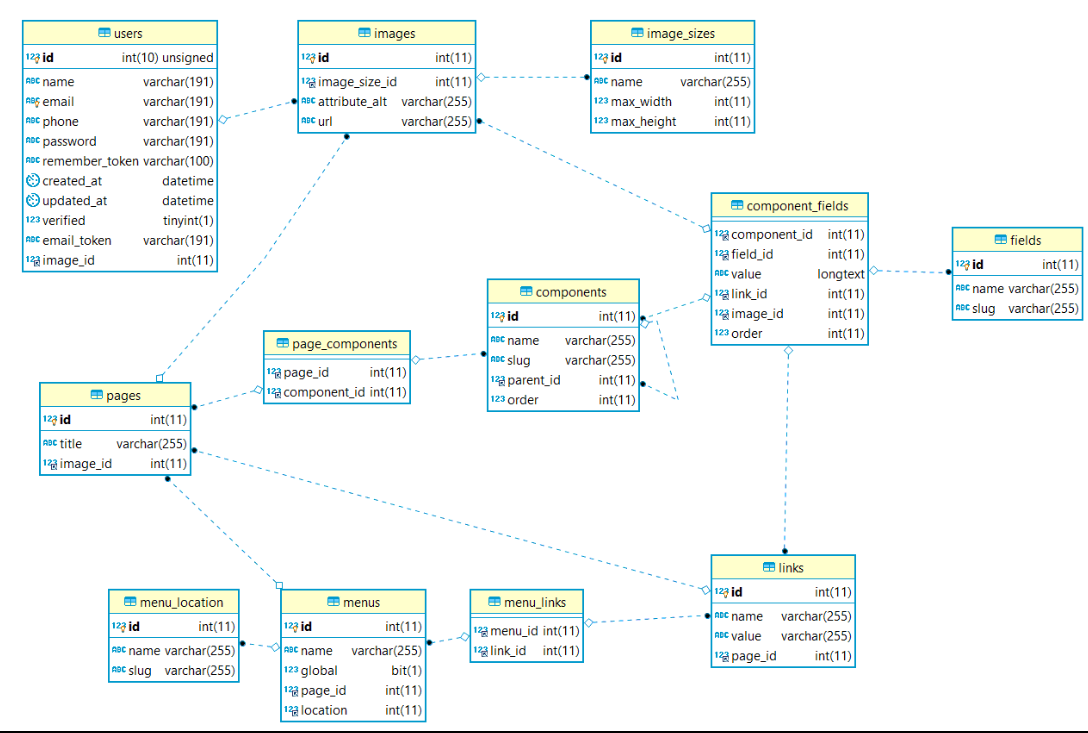
\includegraphics[width=\textwidth]{planlegging-av-database.png}
    \caption{Prosjektets planlagte database}
    \label{fig:database}
\end{figure}

\section{Planlegging av API}
I felleskap begynte vi å planlegge hvilke linker som API-et skal ha, og hva de skal sende i svar. Det ble derfor utarbeidet en JSON-fil som beskriver strukturen og hvilke data den skal gi i svar for forskjellige forespørsler.

I første omgang ble URL-er for Pages og Menus definert. Dataene disse gir i svar, vil være offentlig. 

\lstinputlisting[caption={JSON-eksempel for sider (api.sirkusmedia.no/api/v1/pages)}]{api-code-examples/pages.json}
\lstinputlisting[caption={JSON-eksempel for en side (api.sirkusmedia.no/api/v1/pages/slug)}]{api-code-examples/page.json}
\lstinputlisting[caption={JSON-eksempel for menyer (api.sirkusmedia.no/api/v1/menus)}]{api-code-examples/menus.json}
\lstinputlisting[caption={JSON-eksempel for en meny (api.sirkusmedia.no/api/v1/menus/id)}]{api-code-examples/menu.json}

Denne filen er kun eksempeldata. Den vil bli brukt til å se på at back-end sender svar på riktig måte. Front-end kan også benytte filen og se hvilke svar som kan forventes på de forskjellige forespørselene. Fordelen med dette er at det kan lages \q{dummy responses} som er mulig å jobbe med underveis i utviklingen.

\section{Mockups}
En del av planleggingsfasen var å lage mockups/skisser av nettstedet. Det ble først utarbeidet en skisse for forsiden, slik at den kunne sendes til oppdragsgiver for godkjenning.

\subsection{Versjon 1}
Figur \ref{fig:mockup-v1} viser forsøk nummer 1. Tilbakemeldingen her var oppdragsgiver syns det var et kult design, men ikke helt den stilen de ønsket seg.
\begin{figure}[H]
    \centering
    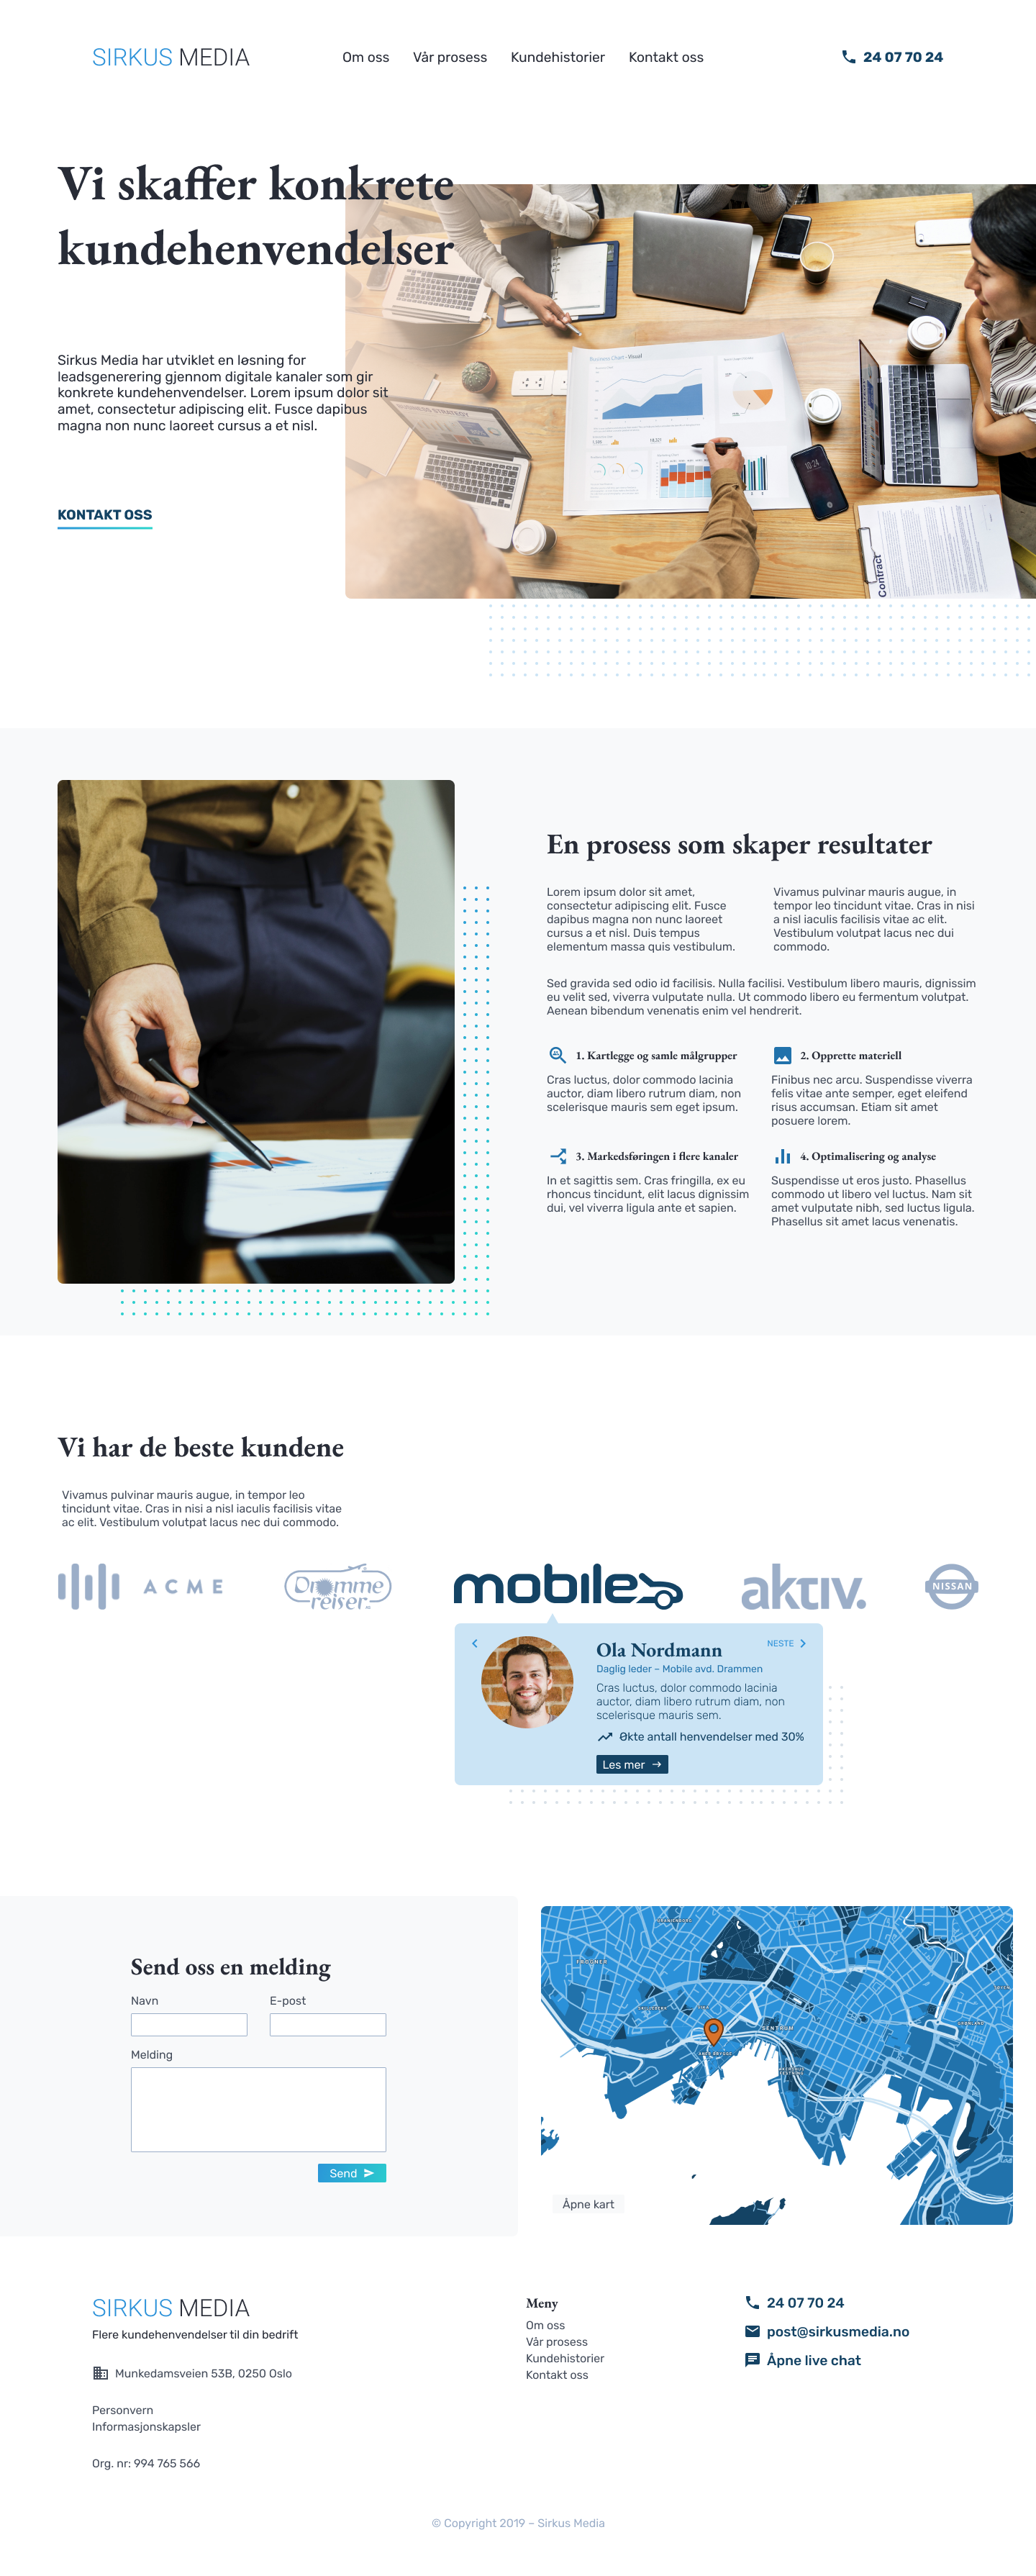
\includegraphics[height=\textheight]{design/mockup1-draft3.png}
    \caption{Mockup - Versjon 1}
    \label{fig:mockup-v1}
\end{figure}

\subsection{Versjon 2}
Figur \ref{fig:mockup-v2} viser forsøk nummer 2. Tilbakemeldingen her var den samme som på versjon 1.
\begin{figure}[H]
    \centering
    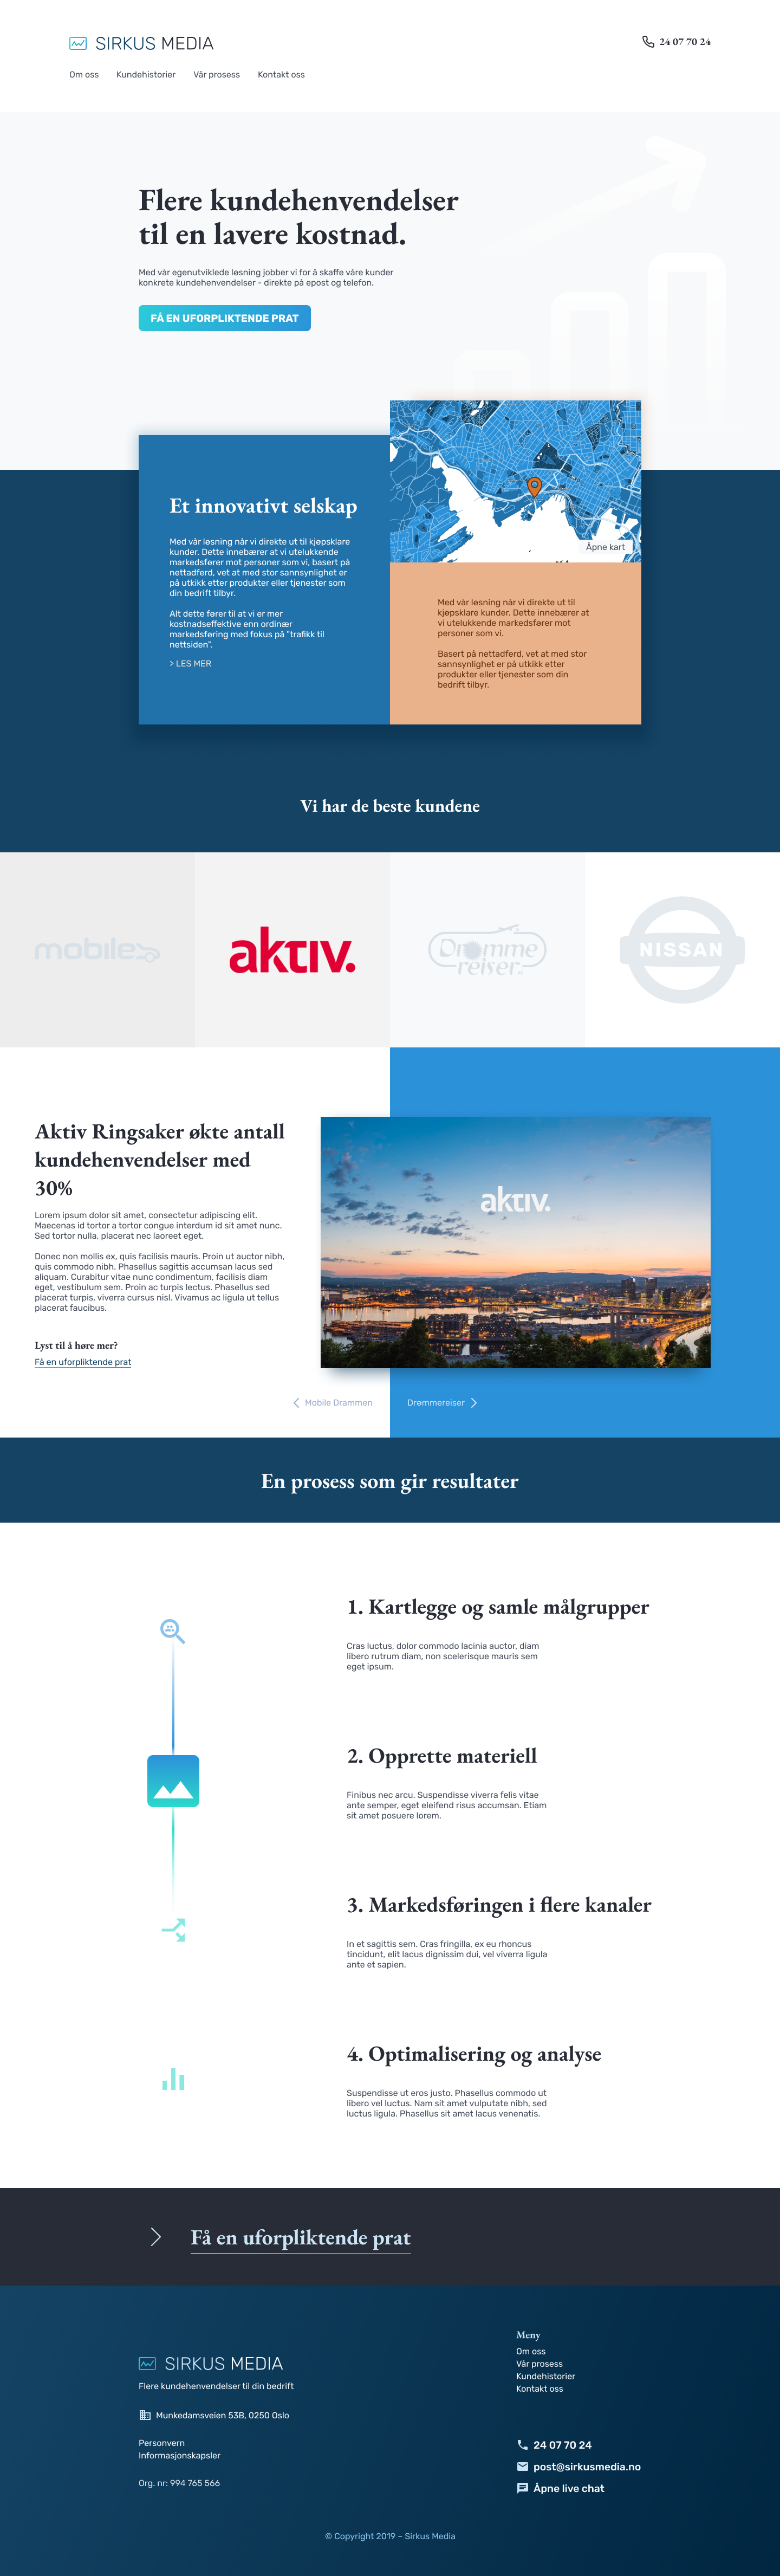
\includegraphics[height=.85\textheight]{design/mockup2-draft3.png}
    \caption{Mockup - Versjon 2}
    \label{fig:mockup-v2}
\end{figure}

\subsection{Versjon 3}
Figur \ref{fig:mockup-v3-index} viser det tredje forsøket. Dette var skissen som ble godkjent.
\begin{figure}[H]
    \centering
    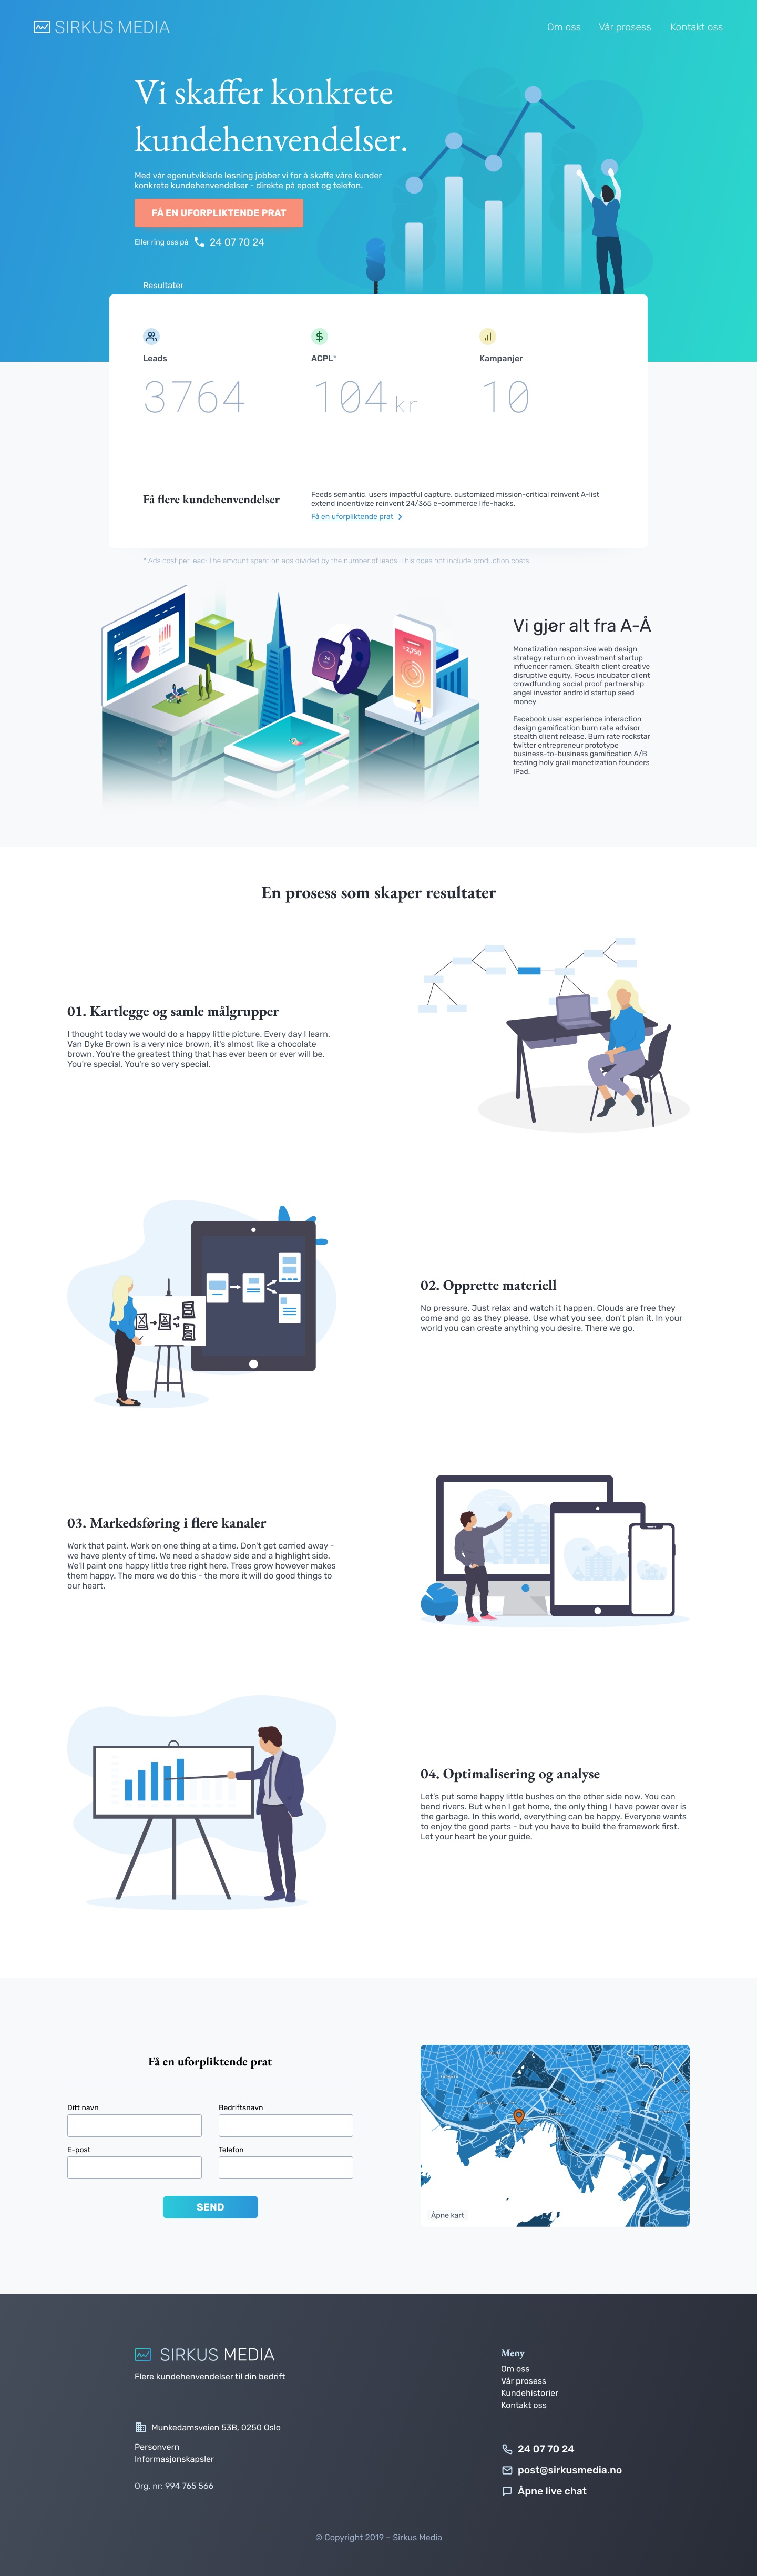
\includegraphics[height=.82\textheight]{design/mockup3-index.png}
    \caption{Mockup - Versjon 3 - Forside}
    \label{fig:mockup-v3-index}
\end{figure}

Når designet til forsiden ble godkjent, startet utarbeidingen av designet til de andre planlagte sidene på front-end.

\textbf{Om oss}

Figur \ref{fig:mockup-v3-about} viser designet til den planlagte \q{Om oss}-siden.
\begin{figure}[H]
    \centering
    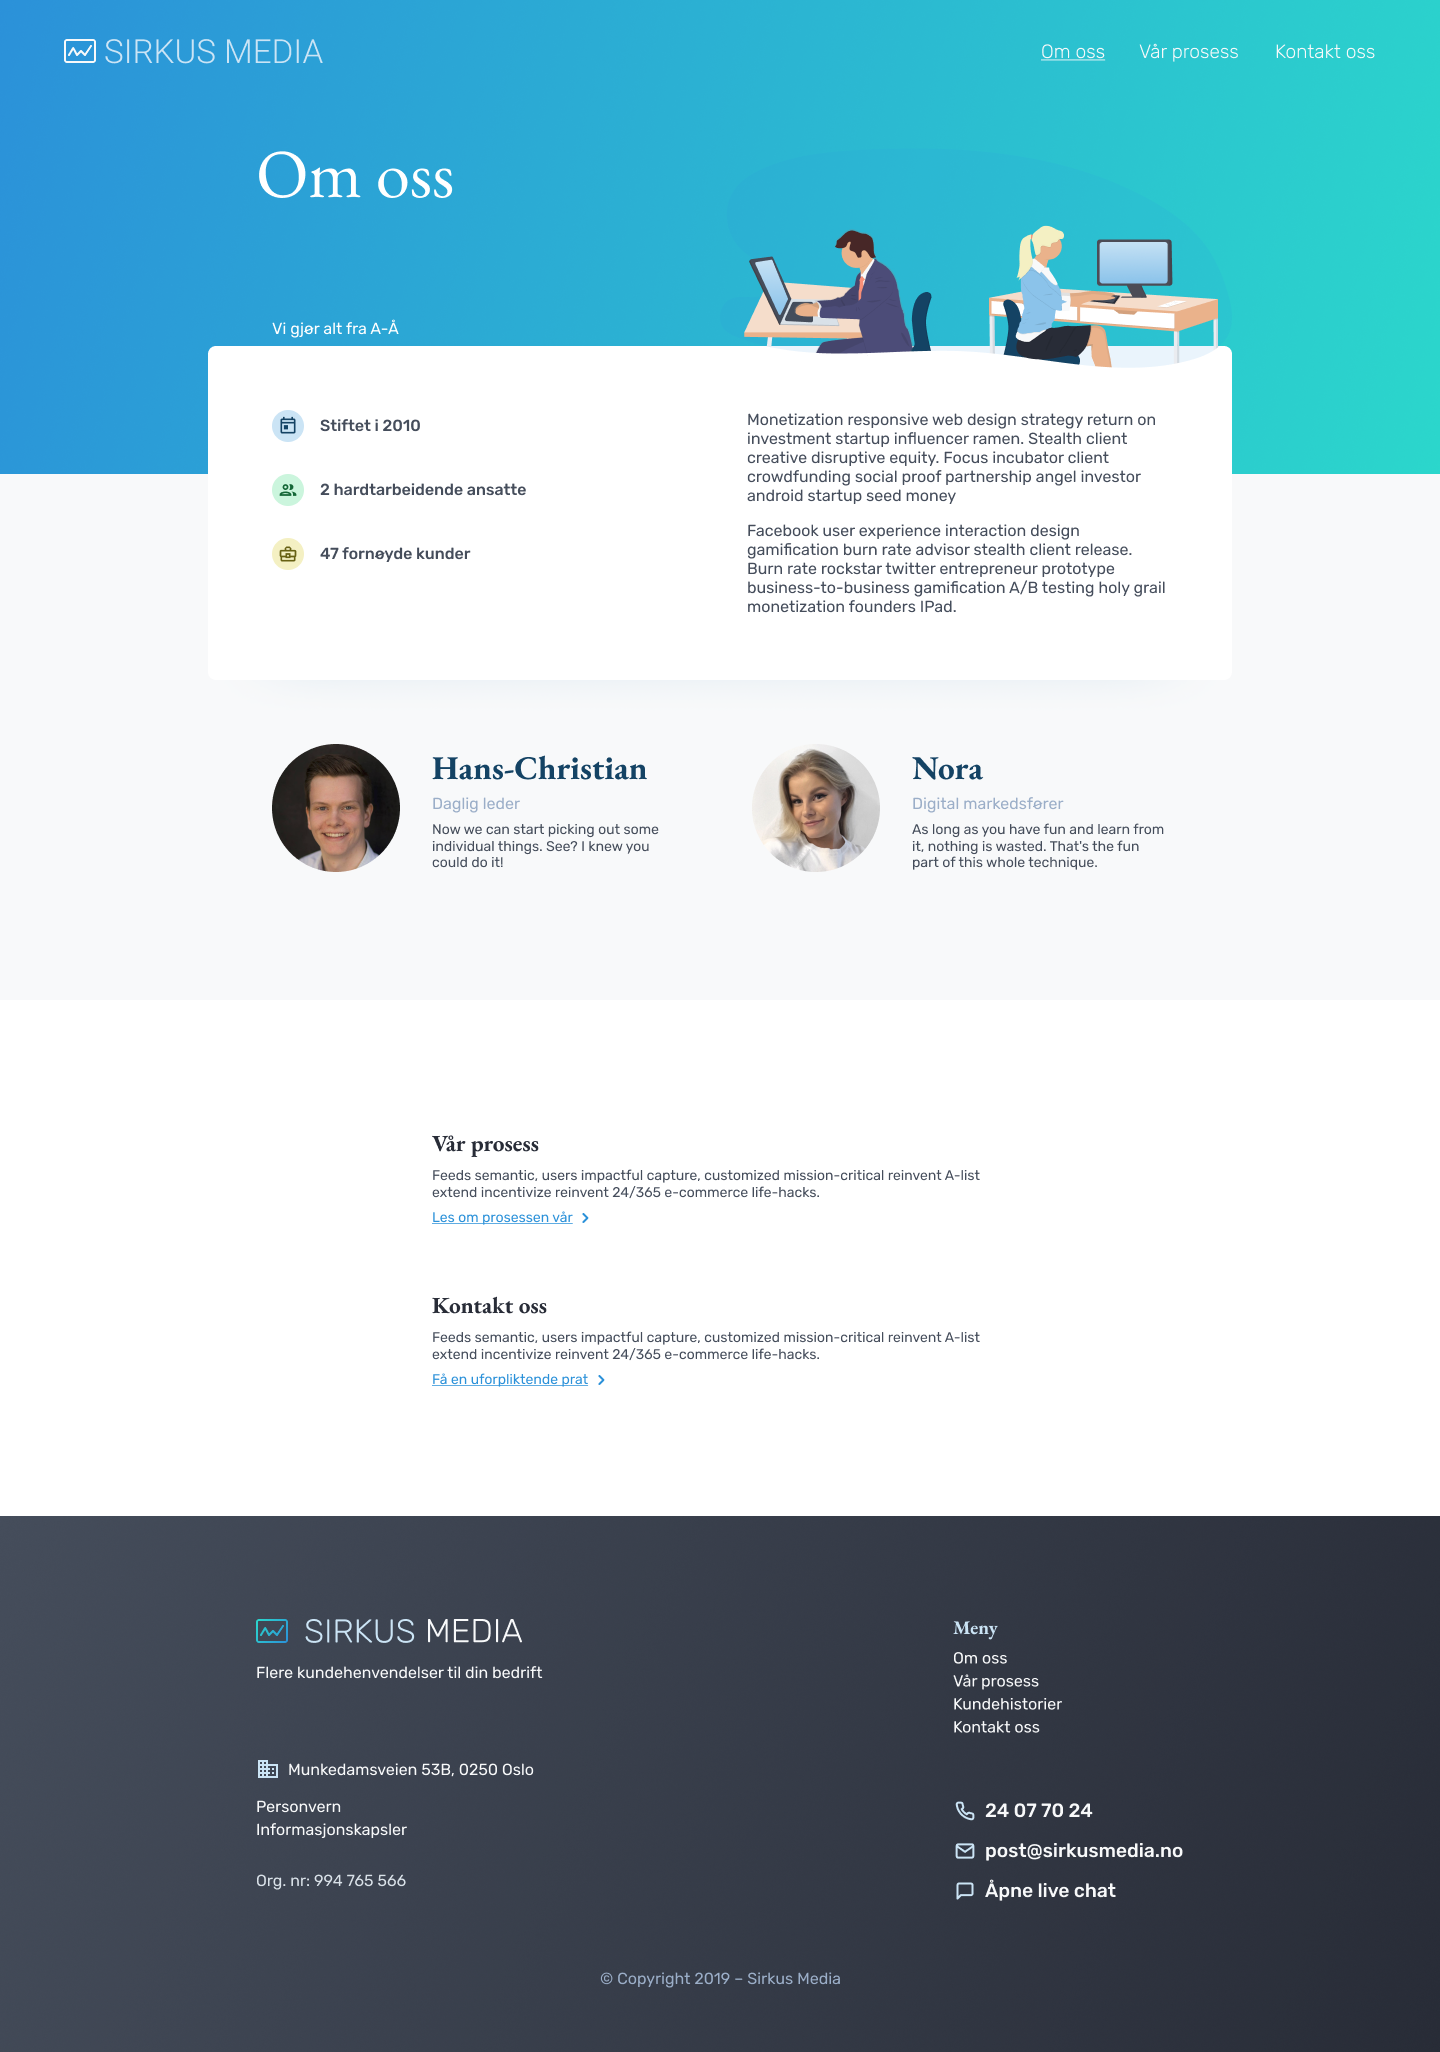
\includegraphics[height=.9\textheight]{design/mockup3-about.png}
    \caption{Mockup - Versjon 3 - Om oss}
    \label{fig:mockup-v3-about}
\end{figure}

\textbf{Kontakt oss}

Figur \ref{fig:mockup-v3-contact} viser designet til den planlagte \q{Kontakt oss}-siden.
\begin{figure}[H]
    \centering
    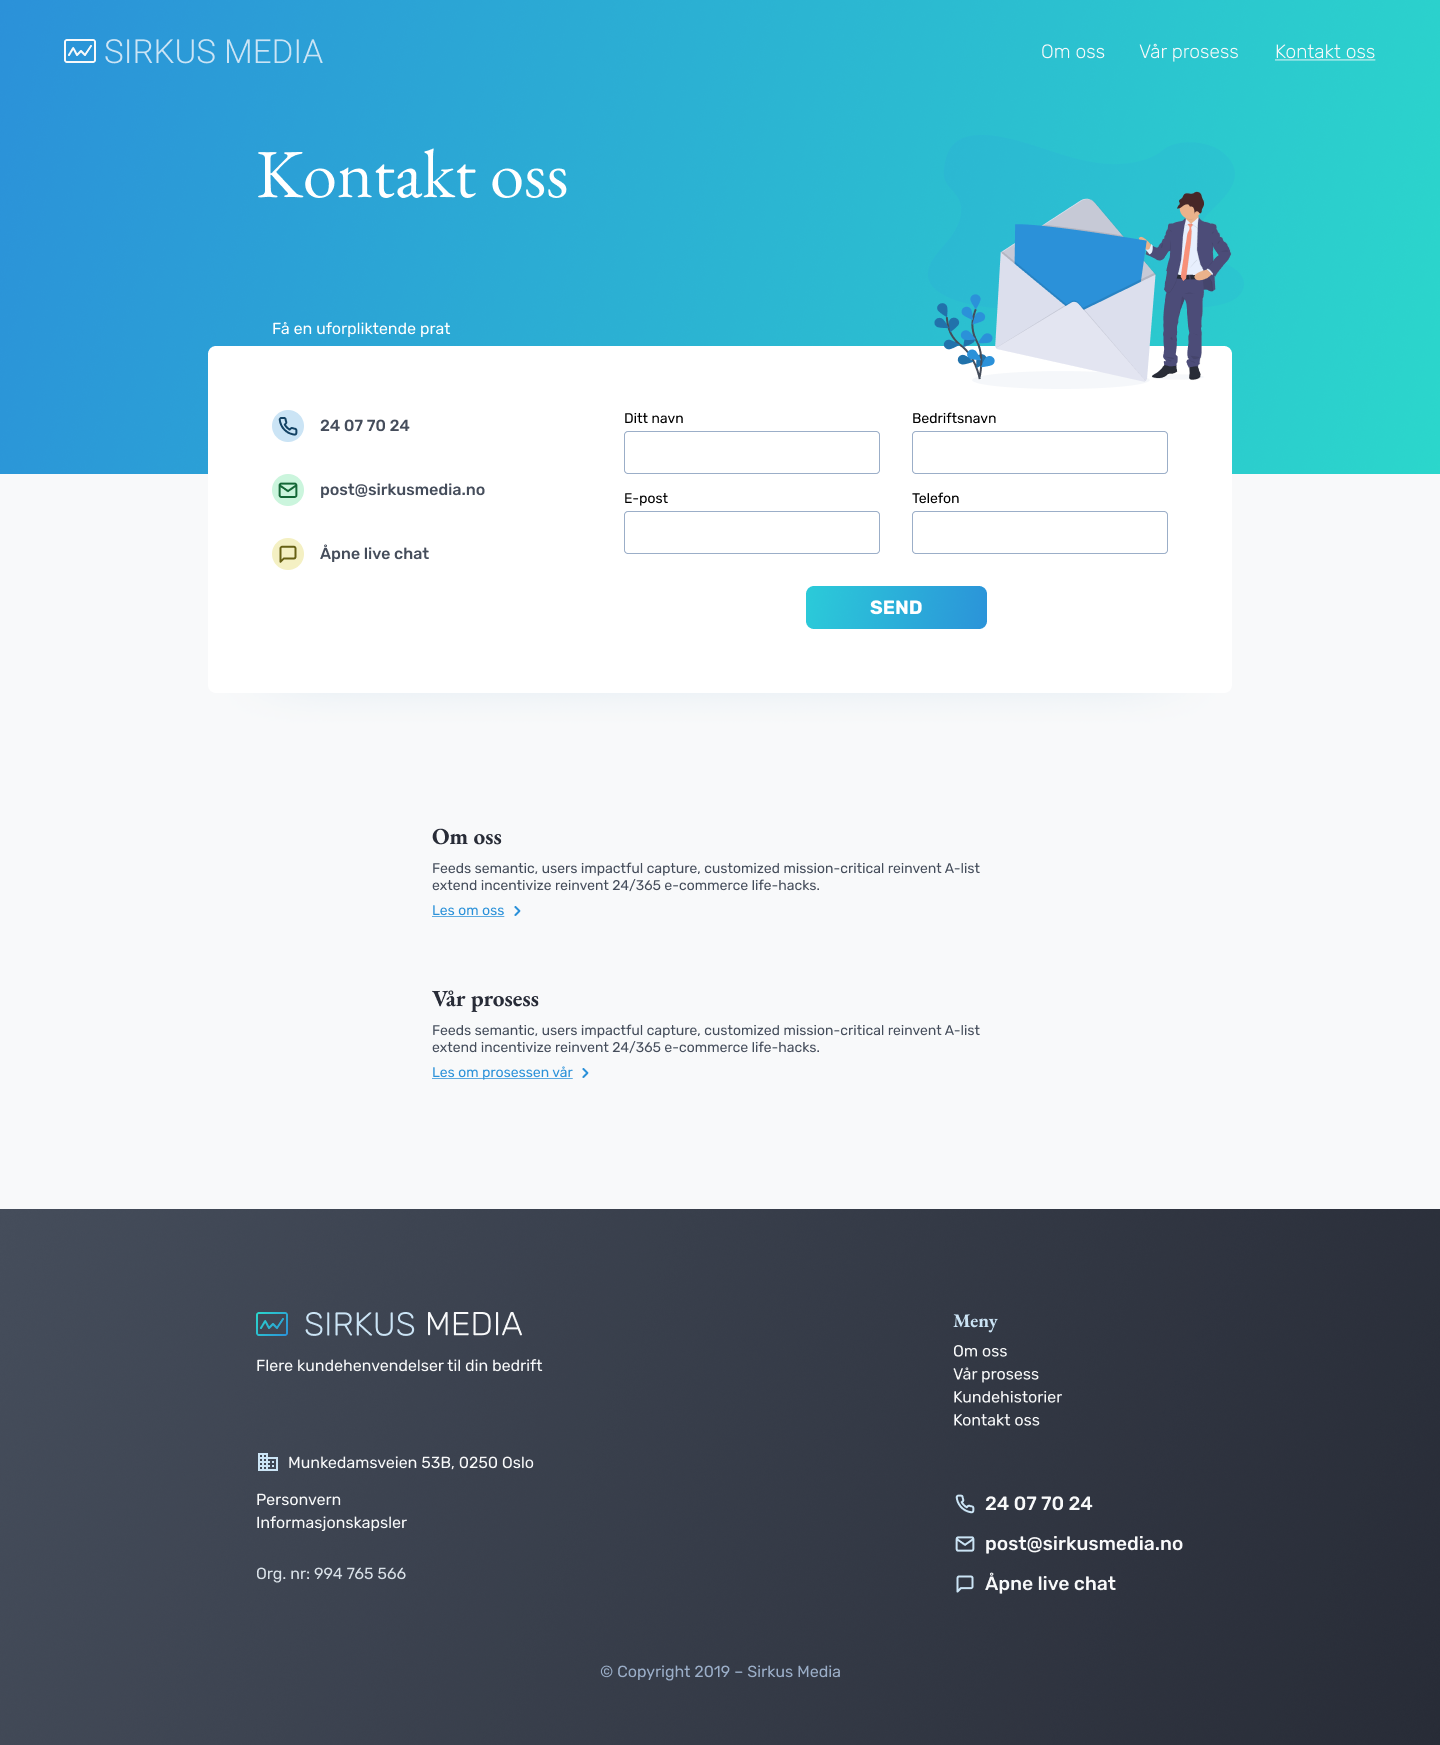
\includegraphics[width=\textwidth]{design/mockup3-contact.png}
    \caption{Mockup - Versjon 3 - Kontakt oss}
    \label{fig:mockup-v3-contact}
\end{figure}

\section{Visuell profil}
Videre ble det opprettet en enkel visuell profil for nettstedet, basert på den godkjente skissen.

\subsection{Logo}
Figur \ref{fig:logo-default} viser logoen som ble utarbeidet. Det ble også laget en lys versjon, se figur \ref{fig:logo-light}.

\begin{figure}[H]
    \centering
    
\includegraphics[width=.5\textwidth]{design/logo.png}
    \caption{Visuell profil - logo}
    \label{fig:logo-default}
\end{figure}

\begin{figure}[H]
    \centering
    
\includegraphics[width=.5\textwidth]{design/logo-light.png}
    \caption{Visuell profil - logo (lys versjon)}
    \label{fig:logo-light}
\end{figure}

\subsection{Ikon}
Figur \ref{fig:icon} viser ikonet som ble utarbeidet.

\begin{figure}[H]
    \centering
    
\includegraphics[width=.25\textwidth]{design/logo-icon.png}
    \caption{Visuell profil - ikon}
    \label{fig:icon}
\end{figure}

\subsection{Farger}
Figur \ref{fig:colors} viser de utvalgte fargene til oppdragsgiver. Disse fargene ble valgt med tanke på å få selskapet til å fremstå som moderne og innovative.
Den midterste kolonnen med farger er standardfargene. Kolonnene til venstre og høyre for midten, er lysere og mørkere versjoner av disse.
\begin{itemize}
    \item Rad en er de forskjellige gråfargene. Disse blir brukt til tekst og bakgrunnsfarger.
    \item Rad to (blå) er primærfargen.
    \item Rad tre (cyan) er sekundærfargen.
    \item Rad fire (grønn) brukes til positive meldinger og handlinger.
    \item Rad fem (gul) brukes til middels negative meldinger og handlinger.
    \item Rad seks (oransje) er aksentfargen.
    \item Rad syv (rød) brukes til sterkt negative meldinger og handlinger.
\end{itemize}

\begin{figure}[H]
    \centering
    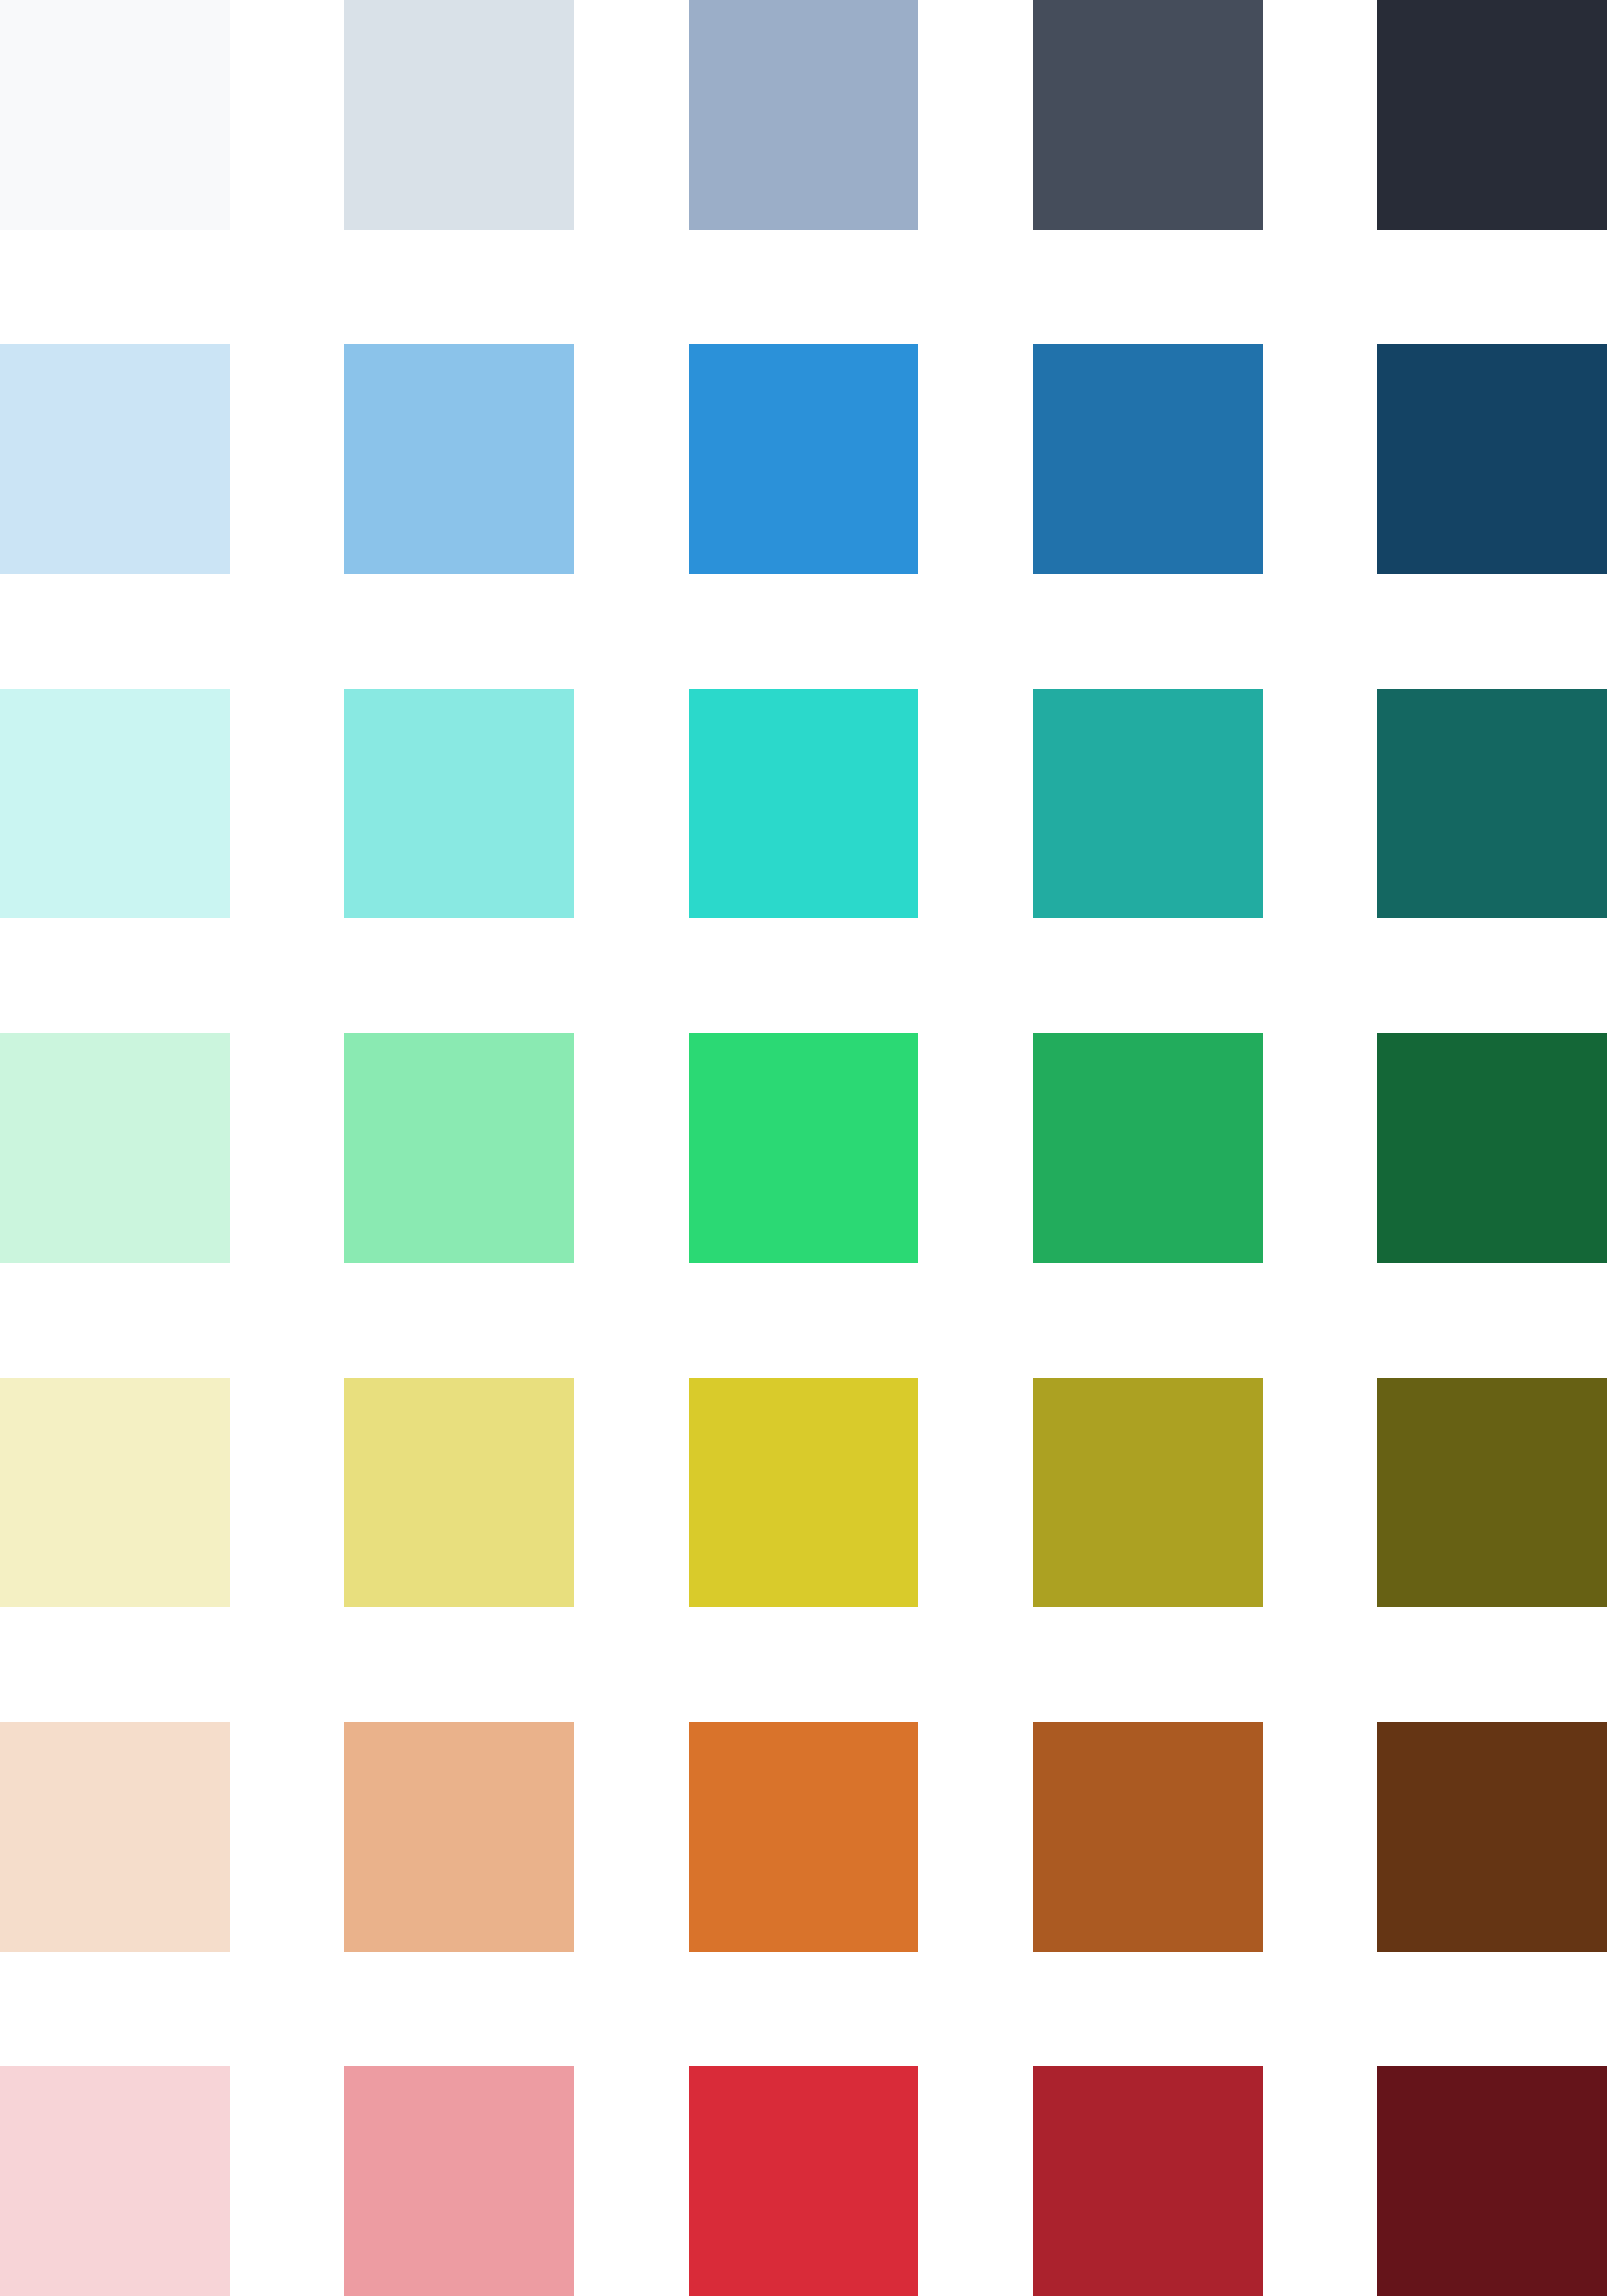
\includegraphics[width=.5\textwidth]{design/colors.png}
    \caption{Visuell profil - farger}
    \label{fig:colors}
\end{figure}

\subsection{Fonter}
Figur \ref{fig:typography} viser fontene som ble valgt til oppdragsgiver.

\begin{figure}[H]
    \centering
    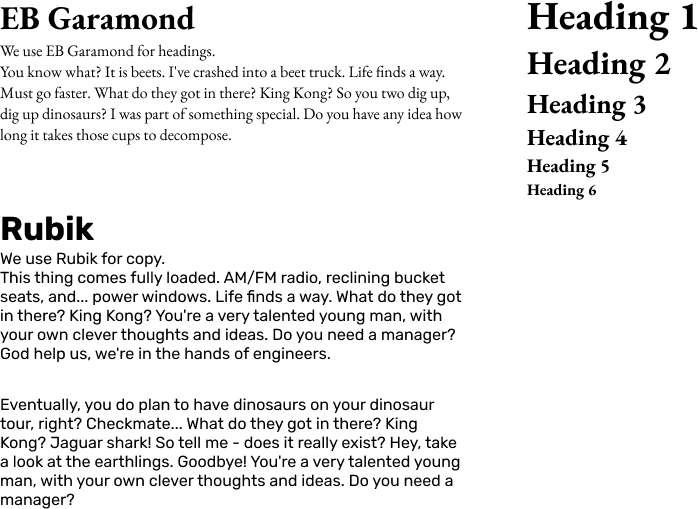
\includegraphics[width=\textwidth]{design/typography.png}
    \caption{Visuell profil - fonter}
    \label{fig:typography}
\end{figure}

% \section{Innhold}

% Vi så Avsnitt \ref{sec:hiof-it}  at man ved HiØ skiller mellom produkt- og prosessdokumentasjon, og operer med flere frittstående dokumenter. Det er ønskelig at hovedokumentet omhandler løsningen av oppdraget, dvs. selve produktet.
% Struktur og innhold bør være som som følger:

% \begin{compactdesc}
% \item [Front Matter]  Som i Avsnitt \ref{sec:mayfield}.

% \item [Body] Hoveddelen av dokumentet (gjennomføringen).
% \begin{compactdesc}
% \item [Introduksjon] Skal gi leseren et bilde av rammene rundt prosjektet: Kort beskrivelse av oppdraget, litt om oppdragsgiver og prosjektgruppen, prosjektets formål, leveranser og metoder. Den bør også inneholde en oversikt over resten av rapporten. 
% \item [Analyse] Kapittelet tar for seg analysedelen av arbeidet. Den består av to hoveddeler, en grundig beskrivelse av oppgaven basert på skissen gitt av oppdragsgiver, og en undersøkelse av hva som finnes av relatert arbeid, {\em best practise} og relevant teknologi. 
% \item [Design]  Basert på beskrivelsen av oppgaven i introduksjonen  og analysen, skal denne delen beskrive hvordan man har tenkt å utforme løsningen. Beskrivelsen er nødvendigvis noe avhengig av type prosjekt. Designet er uavhengig hva slags verktøy man skal bruke i implementasjonen.
% \item [Implementasjon] Her skal det beskrives hvordan man faktisk produserte leveransene i prosjektet, og viktigst, beskrive selve produktet. Hvilke verktøy brukte man, hvordan foregikk produksjonen, etc. Utformingen av dette kapittelet avhenger helt klart av type prosjekt.
% \item [Evaluering] De fleste prosjekter avsluttes med en eller annen form for evaluering av resultatene. I utviklingsprosjekter vil det være naturlig med teknisk testing, fungerer programvaren som den skal? Teknisk testing kan utføres av utviklerne selv, eller en ekstern part, f.eks. oppdragsgiver. En oppdragsgiver ønsker ofte å utføre en akseptansetest, dvs. en test som vil avgjøre om de har "fått det de har betalt for". Ellers vil det i mange tilfeller være nyttig og viktig med en brukertest, dvs. en strukturert test der sluttbrukerne får komme til orde. 
% \item [Diskusjon] Diskusjonskapittelet er viktig, både for dere selv og sensor. Dette kapitelet er det som i hovedsak skiller et akademisk prosjekt fra et rent næringslivsprosjekt. Ble resultatet som forventet? Ble oppdragsgiver fornøyd? Kunne dere gjort noe anderledes/bedre?
% Det er her dere skal dokumentere at dere har lært noe underveis, ikke bare levert et produkt til en oppdragsgiver. 
% \item [Konklusjon] Konklusjon er på et vis et sammendrag av diskusjonskapittelet. Her bør dere legge vekt på de viktigste funnene, både når det gjelder produktet og prosessen. Med et fyldig diskusjonskapittel bør trenger ikke konklusjonen bør være mer enn en side.
% \end{compactdesc}

% \item [Back Matter] Som i Avsnitt \ref{sec:mayfield}.

% \end{compactdesc}

% \section{Utformingen}

% Det følger med en del standard, ferdig definerte stiler med enhver \LaTeX~distribusjon. Disse er gjennomprøvet over flere 10-år, og har tålt tidens tann både teknisk og estetisk. Når man skal lage sine egne design, vil det som regel alltid være fornuftig å gå ut i fra en  av standardstilene. Det gjør vi også i dette prosjektet, og tar utgangspunkt i stilen {\em report}, parametrisert for dobbeltsidig A4-format, med 11pt basis fontstørrelse. Vi foreslår følgende endringer i report-stilen: 

% \paragraph{Marger}
% I følge egen og kollegers erfaring er marginene noe store i standardrapporten, slik at det blir litt ``trangt'' for tekst, tabeller og illustrasjoner. Vi foreslår en layout med reduserte marger på alle sider.


% \paragraph{Topptekst / bunntekst}
% Når man slår opp en dobbeltsidig bok, kalles venstre side for {\em verso}, og høyre for {\em recto}.
% \index{Recto}
% Vi ønsker at bunnteksten skal være uten andre elementer enn fotnoter. Sidetallet bør trykkes i toppteksten, til venstre på verso sider, og til høyre på recto sider. På denne måten
% blir det lett å bla fort igjen for å finne et gitt sidetall,  som f.eks. er funnet i en indeks. Videre er det ønskelig at aktuelt kapittel er angitt til høyre på verso sidene, og aktuelt underkapittel til venstre på recto sidene.

% \paragraph{Tittelsiden} 
% Det skal være to tittelsider, først en fengende forside, som studentene utformer selv, og deretter en standard bacheloroppgave-side som er lik for alle.


% \section{Leveransene og malen}
% Første versjon av hoveddokumentet  bør bestå av introduksjonen og analyse- og designkapitlene (Kapittel \ref{chap:intro}, \ref{chap:analysis} og Kapittel \ref{chap:design}), og andre versjon bør være en mer eller mindre komplett beskrivelse av selve resultatet (Kapittel \ref{chap:implementation}). Endelig leveranse tilsvarer den komplette rapporten pluss selve produktet (og poster og presentasjon).






    \cleardoublepage
\chapter{Produksjon av CMS og nettsted}
\label{chap:implementation} 

% \meta{
% Her skal det beskrives hvordan man faktisk produserte resultatene i prosjektet, og viktigst, beskrive selve produktet. Hvilke verktøy brukte man, hvordan foregikk produksjonen, etc. Utformingen av dette kapittelet avhenger helt klart av type prosjekt.
% }

I dette kapittelet skal vi presentere resultatene i prosjektet og beskrive CMS og nettstedet. Her vil vi også presentere hvilke verktøy vi endte opp med å bruke og hvordan selve produksjonen foregikk.

\section{Verktøy}
Vi endte opp med å bruke flere verktøy enn beskrevet i  \ref{sec:technologies}. 
I tillegg til hovedverktøyene ble følgende verktøy og teknologier benyttet:

\subsection{GNU/Linux}
GNU/Linux er en familie med Unix-lignende operativsystemer som baserer seg på Linux-kjernen \cite{kernel_org} og en del programvare fra GNU-prosjektet \cite{gnu_org}. I denne familien finner vi blant annet Ubuntu, Debian, Fedora, Red Hat Linux og Arch Linux.

I dette prosjektet blir GNU/Linux benyttet som operativsystem på serveren som \q{hoster} back-end.

\subsection{MySQL}
MySQL \cite{oracle2019am} er et databasestyringssystem med åpen kildekode.

Prosjektets database er en MySQL-database.

% \subsection{Let’s Encrypt}
% Let’s Encrypt \cite{le2019ale} er en gratis og åpen sertifikatautoritet som gir ut X.509-sertifikater for kryptering av transportlaget. Tjenesten leveres av ISRG (Internet Security Research Group).

% Studentgruppen har benyttet Let's Encrypt til å lage TLS-sertfikater\footnote{Se avsnitt \ref{sec:analysis-security-tls}}.

\subsection{Node.js}
Node.js er et servermiljø med åpen og gratis kildekode. Node.js kan kjøre på ulike plattformer (Windows, Linux, Unix, Mac OS X) og bruker JavaScript på serveren \cite{w3schools2019win}. I tillegg kan Node.js generere dynamisk sideinnhold og opprette, åpne, lese, skrive, slette og lukke filer på serveren. I tillegg kan Node.js legge til, slette og endre data i databasen.

Vi har brukt Node.js for å kunne kjøre verktøy knyttet til utvikling av front-end.

\section{Tilhørende teknologier og begreper}
Ved å bruke verktøyene som har blitt presentert benyttes også noen tilhørende teknologier. Disse blir presentert videre i dette kapittelet. 

\subsection{Git}
Git \cite{TechTarget} er et system for versjonskontroll. Et versjonskontrollsystem blir hovedsaklig brukt under utvikling av software og nettsteder. Det kan også brukes til andre type prosjekter som grafisk design og skriving av dokumenter.

Ved å bruke Git har vi fått en historikk over alle endringer, samt en sikkerhetskopi av alle versjoner av filene. En annen fordel ved å bruke Git er at det blir enklere å samarbeide med hverandre, uten å måtte tenke på at alle må sitte på nyeste versjon av filene.

% \subsection{Github}
% GitHub.com er et nettsted for å hoste git repositories, og blir mye brukt for \q{Open Source}-prosjekter. 

% Github \cite{TechTarget} er et sentralisert punkt for å samle en brukers repositories. Ved siden av å hoste repositories, lar GitHub brukere dele repositories med hverandre, lage informasjonssider om prosjektet og opprette saker (issues).

% \subsection{HTTP/2}
% HTTP/2 \cite{Belshe2015httpv} er en revisjon av HTTP-nettverksprotokollen. HTTP er et sett med regler for overføring av filer (tekst, grafiske bilder, lyd, video og andre mediefiler). Et av de store målene med HTTP/2 var å tillate multipleksing.

\subsection{REST-API}
Et API (programmeringsgrensesnitt) er et sett med funksjoner, prosedyrer, metoder eller klasser som brukes av dataprogrammer for å be om tjenester fra operativsystemet eller programvare som er på datamaskinen. En programmerer kan bruke API-er til å lage applikasjoner.

REST (Representational State Transfer) er en arkitektonisk stil for programvare. Et REST-API \cite{Masse2011radr} er et API som følger REST-stilen og de begrensninger som REST definerer.

\subsection{Google Analytics}
\label{sec:google-analytics}
Google Analytics \cite{google2019gtk} er en gratis, webbasert tjeneste som gir statistikk og grunnleggende verktøy for analyse av bruksdata, søkemotoroptimalisering og markedsføring.

Dette verktøyet blir av oss brukt til å overvåke hvordan brukerne på nettsiden oppfører seg.

\section{Utviklingen}

Det ble opprettet en \q{Branch protection rule} på back-end repository i Github. Dette gjør at det må kjøres en \q{Code review} før kode kan sendes inn til \q{Master branch}-en. Alle medlemmene på studentgruppen har en egen branch.
Når koden skal commites må det opprettes en pull request, som må godkjennes. Da blir det mulig å luke ut kode som inneholder feil som potensielt kan ødelegge for eksisterende kode.

\section{Back-end}
\subsection{Installasjon og oppsett av Laravel og tilhørende verktøy}
Første steg var å installere package manageren Composer. Deretter kunne siste versjon av Laravel (5.7) settes opp og installeres. Da vi benyttet oss av Composer ble det mulig å installere Laravel med et par kommandoer i terminalen:
\begin{lstlisting}[caption={Installasjon av Laravel med Composer},language=bash]
    composer global require laravel/installer
    laravel new sirkus-media-back-end
\end{lstlisting}

Til slutt måtte vi konfigurere rammeverket slik at det kunne håndtere databasetilkobling, sending av e-post og lagring av opplastede og genererte filer. Laravel samler sine innstillinger i PHP-filer i \q{config} mappen, samt en .env fil som holder på passord og annen sensitiv informasjon vi ikke vil ha i git.

\subsubsection{Database}
Vi begynte med å sette opp tilkobling til databasen. Dette ble gjort ved å først logge inn i MySQL og opprette en bruker og en database. Informasjon for dette ble skrevet inn i .env filen. Se figur under for eksempel:
\begin{lstlisting}[caption={Laravel .env database secrets},language=bash]
    DB_CONNECTION=mysql
    DB_HOST=127.0.0.1
    DB_PORT=3306
    DB_DATABASE=sirkusmedia
    DB_USERNAME=bruker
    DB_PASSWORD=passord
\end{lstlisting}

\subsubsection{Mail}
Etter at databasen var klar for bruk begynte vi å sette innstillingene for e-post. Vi bestemte oss for å bruke Mailtrap\footnote{\url{https://mailtrap.io/}} under utvikling av løsningen. Mailtrap\cite{mailtrap2019setfsad} er en uekte SMTP-server som kan brukes for testing av e-post. Etter å ha registrert bruker hos Mailtrap fylte vi ut følgende informasjon i .env filen:
\begin{lstlisting}[caption={Laravel .env mail secrets}, language=bash]
    MAIL_DRIVER=smtp
    MAIL_HOST=smtp.mailtrap.io
    MAIL_PORT=2525
    MAIL_USERNAME=bruker
    MAIL_PASSWORD=passord
    MAIL_ENCRYPTION=tls
\end{lstlisting}

Når løsningen skal ut i produksjon må det brukes noe annet enn Mailtrap. Sirkus Media kan selv bestemme hva de ønsker å bruke, men systemet er satt opp til bruk av Mailgun\footnote{\url{https://www.mailgun.com/}}.

\subsubsection{Lagring}
Lagring av opplastede og genererte filer foregår på samme server som back-end kjører på. For å sette opp dette kjørte vi en Larvel Artisan kommando:
\begin{lstlisting}[caption={Laravel Artisan kommando for å sette opp lagring av filer}, language=bash]
    php artisan storage:link
\end{lstlisting}
Storage klassen til Larvel gjør at Sirkus Media enkelt kan benytte seg av andre løsninger, som for eksempel Amazon Web Servies S3.

\subsubsection{Laravel Mix}
Laravel Mix\footnote{\url{https://laravel-mix.com/}} var det siste som måtte settes opp før utviklingen kunne starte. Dette er en \textit{wrapper} rundt den populære module bundleren Webpack\footnote{\url{https://webpack.js.org/}}. For å bruke Laravel Mix måtte vi først installere Node.js. Etter Node.js ble installert trengte vi kun å kjøre et par npm-kommandoer:
\begin{lstlisting}[caption={npm-kommando for å sette opp front-end til Laravel}, language=bash]
    npm install
    npm run dev
\end{lstlisting}

For å konfigurere hvilke filer som skal brukes av front-end til Laravel fylte vi ut filen webpack.mix.js:
\begin{lstlisting}[caption={Eksempel på oppsett av webpack.mix.js}]
    const mix = require("laravel-mix");

    mix.sass("resources/sass/app.scss", "public/css").version();
    mix.js("resources/js/app.js", "public/js").version();
    mix.copy("resources/images", "public/images").version();

    mix.browserSync({ proxy: "localhost:8000", notify: false });
\end{lstlisting}

Når vi snakker om \q{front-end til Laravel}, er det ikke snakk om front-end til nettsiden som lages for Sirkus Media, men front-end til CMS-et.
Laravel kommer med en del dependencies til front-end som vi ikke trenger. Alle dependencies defineres i package.json. Følgende dependencies ble fjernet: Bootstrap, jQuery, lodash, Popper og Vue. Det ble kun lagt til en dependency; Shopify sin Draggable pakke. BrowserSync ble også lagt til som en devDependency.

\begin{lstlisting}[caption={Orginal package.json}]
    "devDependencies": {
        "axios": "^0.18",
        "bootstrap": "^4.0.0",
        "cross-env": "^5.1",
        "jquery": "^3.2",
        "laravel-mix": "^4.0.7",
        "lodash": "^4.17.5",
        "popper.js": "^1.12",
        "resolve-url-loader": "^2.3.1",
        "sass": "^1.15.2",
        "sass-loader": "^7.1.0",
        "vue": "^2.5.17"
    },
    "dependencies": {}
\end{lstlisting}

\begin{lstlisting}[caption={Siste package.json}]
    "devDependencies": {
        "browser-sync": "^2.26.3",
        "browser-sync-webpack-plugin": "^2.0.1",
        "cross-env": "^5.1",
        "laravel-mix": "^4.0.7",
        "resolve-url-loader": "^2.3.1",
        "sass": "^1.15.2",
        "sass-loader": "^7.1.0",
        "vue-template-compiler": "^2.6.10"
    },
    "dependencies": {
        "@shopify/draggable": "^1.0.0-beta.8",
        "axios": "^0.18.0"
    }
\end{lstlisting}
Den eneste grunnen til at vue-template-compiler ligger som en dependency her, er fordi siste versjon av Laravel Mix ikke kjører uten.

\subsection{Modeller og database migrations}
Definering av modeller og migrasjon filer til databasetabellene var det første som ble gjort etter konfigurering av rammeverket.
Modeller lagde vi ved å skrive følgende Larvel Artisan kommando i terminalen:
\begin{lstlisting}[caption={Laravel Artisan kommando for oppretting av modell og migration},language=php]
    php artisan make:model Modelnavn -m
\end{lstlisting}
Parameteret \q{-m} i kommandoen over brukes for å opprette en migration-fil for modellen. Det er også mulig å opprette migration-fil etter å ha lagd en modell:
\begin{lstlisting}[caption={Laravel Artisan kommando for oppretting av migration fil},language=php]
    php artisan make:migration migration_file_name
\end{lstlisting}
Etter at modellene og migration filene er opprettet kan man definere forhold mellom modellene (gjøres i modell filen), samt databasetabell for hver modell (gjøres i migration filen).
Når migration filene er ferdig definert kan man kjøre migration ved å skrive følgende kommando i terminalen:
\begin{lstlisting}[caption={Laravel Artisan kommando for å kjøre migration},language=php]
    php artisan migrate
\end{lstlisting}
Etter at migration blir kjørt vil alle tabellene og deres kolonner bli opprettet i MySQL.
Under er et eksempel på en migration fil
\lstinputlisting[caption={Laravel migration fil}, language=php]{laravel-code-examples/migration.php}

\subsubsection{Eloquent forhold mellom modellene}
Eloquent\footnote{\url{https://laravel.com/docs/5.8/eloquent}} er Laravel sitt ORM, det lar oss definere forhold mellom de forskjellige modellene. Det er ønskelig å definere forhold som f.eks: en forfatter har mange bøker. Når et slikt forhold er definert i modellene til Larvel, lar Eloquent oss hente alle bøkene til forfatteren med kode som dette: \lstinline[language=PHP]{$author->books}.

For å definere slike forhold brukte vi de innebygd metodene til Laravel som: belongsToMany, hasOne, belongsTo og hasMany. For eksempel av bruk, se følgende kode:
\lstinputlisting[caption={Laravel modell med et forhold}, language=php]{laravel-code-examples/model-relationship.php}

\subsubsection{Test av migration filer}
Første gang vi kjørte migration dukket det opp en feil:
\begin{lstlisting}[caption={Feilmelding i Laravel ved kjøring av migration},language=PHP]
Illuminate\Database\QueryException : SQLSTATE[42000]: Syntax error or access violation: 1071 Specified key was too long; max key length is 767 bytes (SQL: alter table `users` add unique `users_email_unique`(`email`))
\end{lstlisting}
Denne feilen viste seg å være relativt vanlig og kom av at vi kjørte en eldre versjon (5.7) av MySQL som ikke støtter datatypen varchar med lengde på 255, når collation til databasen er satt til UTF8MB4. Løsningen her ble å sette standard varchar lengde til 191.
\begin{lstlisting}[language=PHP, caption={Definering av standard varchar lengde i AppServiceProvider.php}]
    <?php

    class AppServiceProvider extends ServiceProvider
    {
        public function boot()
        {
            Schema::defaultStringLength(191);
        }
    }
\end{lstlisting}

\subsubsection{Test av forhold mellom modellene}
Når alle forhold var ferdig definert og migration-filene kjørte uten feil, fylte vi databasen med data for å teste at alle forhold var riktig satt opp. Da støtte vi på en feil relatert til vår bruk av UUID som primærnøkkel i stedet for en inkrementerende integer i flere av modellene. Når vi forsøkte å lagre en modell til databasen fikk vi denne feilen:
\begin{lstlisting}[language=PHP]
    SQLSTATE[HY000]: General error: 1364 Field 'id' doesn't have a default value ...
\end{lstlisting}

Feilen kom av hvordan Laravel har satt opp standardmodellen alle modeller baserer seg på. Vi måtte derfor finne en måte å si at alle modeller som brukte UUID har primærnøkkel av typen string, ikke skal inkrementeres. Samtidig skal det genereres en UUID automatisk ved lagring. Den beste måten vi fant å gjøre dette på var ved å lage en trait. Følgende fil ble opprettet:
\lstinputlisting[caption={Trait for å håndtere UUID for Larvel-modeller}, language=php]{laravel-code-examples/trait-uuid.php}

Nå som trait-en var definert, kunne vi inkludere den i alle modeller som brukte UUID som primærnøkkel. Dette blir vist i koden under. Problemet var dermed løst.
\begin{lstlisting}[caption={Bruk av UUID trait i modell}, language=PHP]
    <?php

    use App\Traits\UsesUuid;

    class User ...
    {
        use UsesUuid;

        ...
    }
\end{lstlisting}

Etter de overnevnte problemene ble løst, støtte vi ikke på noen flere nevneverdige problemer rundt forhold mellom modeller.

\subsection{Oppsett av autentisering}
Med databasen og forhold mellom modeller på plass, var vi klare for å begynne utviklingen av selve CMS-et. Vi bestemte oss for å først sette opp autentisering da dette er enklere å implementere fra starten av, fremfor å gjøre det til slutt.
Laravel gir oss mye hjelp på dette området. Ved å kjøre en kommando settes alt vi trenger opp:
\begin{lstlisting}[language=PHP]
    php artisan make:auth
\end{lstlisting}
Etter å ha kjørt kommandoen over, fikk vi de nødvendige controllere og views for innlogging og registrering av brukere, samt system for tilbakestilling av passord.

\subsubsection{Brukerroller}
Selv om autentiseringen var klar, hadde vi ingen måte å skille rettighetene til de forskjellige brukerene på. Dette er heller ikke funksjonalitet som følger med Laravel. Vi fant derfor en PHP pakke: Laravel-Permission\footnote{\url{https://github.com/spatie/laravel-permission}} fra Spatie. Denne pakken utvider Laravel til å støtte brukerroller og kan installeres med Composer. Laravel-Permission gjør det mulig å opprette roller og knytte rettigheter til hver rolle. Vi definerte kun roller og satte følgende: superadmin, admin, moderator og user.
\begin{itemize}
    \item User endte opp med å ikke bli brukt, ligger forsatt tilgjengelig for å gjøre det enklere å utvide systemet videre.
    \item Moderator har tilgang til å opprette, redigere og slette sider og menyer.
    \item Admin har samme tilgang som moderator og kan i tilleg registrere nye brukere.
    \item Superadmin har tilgang til alt. Det vil si at de i tillegg til å kunne gjøre alt det overnevnte, kan lage komponenter, felter og meny lokasjoner, samt at de kan definere hvilke felter en komponent skal ha.
\end{itemize}


\subsection{API}
Vi definerte et API som lot oss hente data fra CMS-et og bygge front-end. Det ble satt opp en prefix for alle API-forespørsler, slik at systemet kan videreutvikles uten å ødelegge for eksisterende løsninger. Alle forespørsler til API-et må starte med /api/v1.

API-et krever ingen autentisering, men forespørsler tillates kun fra spesifikke \textit{origins}. Når prosjektet settes ut i produksjonsmiljø vil forespørsler kun tillates fra \url{https://sirkusmedia.no} og \url{https://www.sirkusmedia.no}. Dette defineres i .env filen.

Følgende lenker kan hentes ut:
\begin{itemize}
  \item pages - Henter ut en liste med alle sider. Hver side i listen holder følgende: id, slug, link, tittel, bilde, dato den ble opprettet og dato som den sist ble redigert.
  \item pages/\{\{slug\}\} - Henter ut en spesifikk side. Den inneholder data om alle komponentene som er på siden, og verdien til feltene til komponentene.
  \item menus - Henter ut en liste med alle menyer og deres lokasjon.
  \item menus/\{\{ID\}\} - Henter ut en spesifikk meny. Her vil alle linker som menyen har, følge med.
\end{itemize}

\section{Oppsett av chat}
Vi bestemte oss for å sette opp en livechat løsning fra Hubspot\footnote{\url{https://www.hubspot.com/products/crm/live-chat}}. Figur \ref{fig:chat-user} viser hvordan det ser ut for sluttbruker. Figur \ref{fig:chat-admin} viser hvordan det ser ut for administrator.
\begin{figure}[H]
    \begin{center}
        \subfigure[Chat når en bruker kommer inn på nettstedet]{
            \label{fig:chat-init}
            \frame{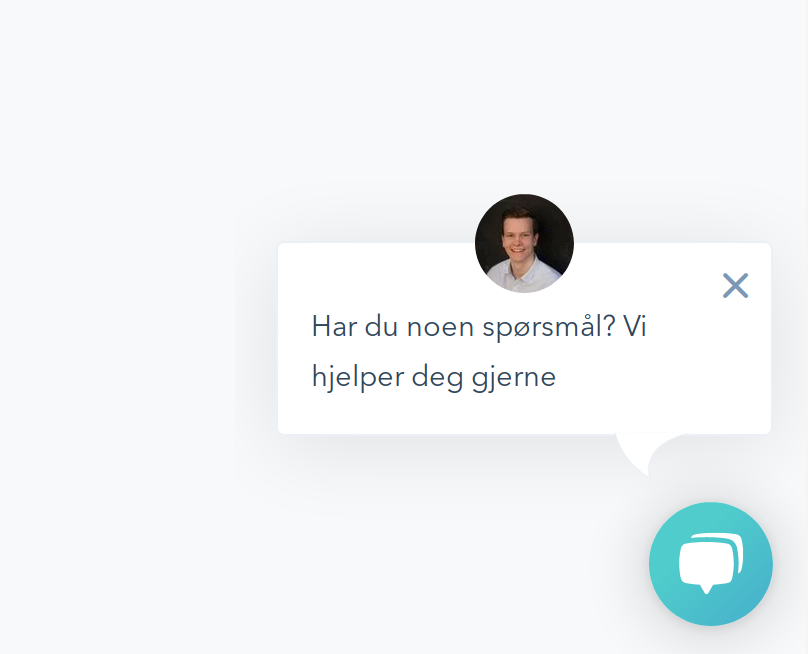
\includegraphics[width=0.47\textwidth]{bjornar/chat-init.png}}
        }
        \subfigure[Chat åpnet]{
            \label{fig:chat-open}
            \frame{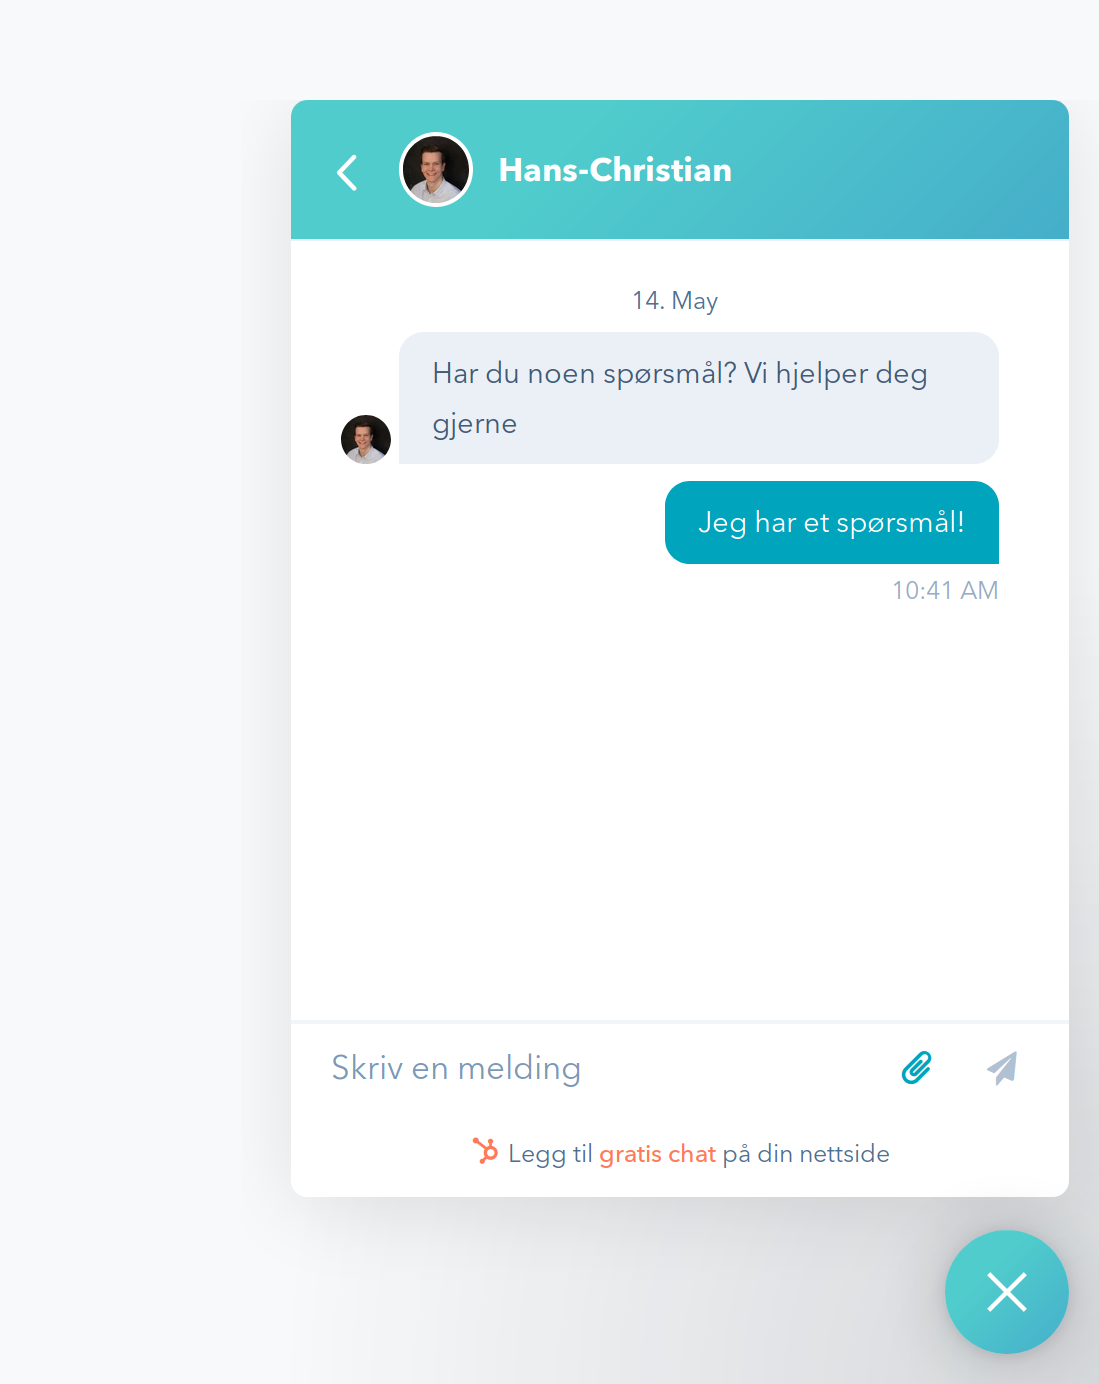
\includegraphics[width=0.3\textwidth]{bjornar/chat-open.png}}
        }
        \label{fig:chat-user}
        \caption{Chat for bruker}
    \end{center}
\end{figure}
\begin{figure}[H]
    \centering
    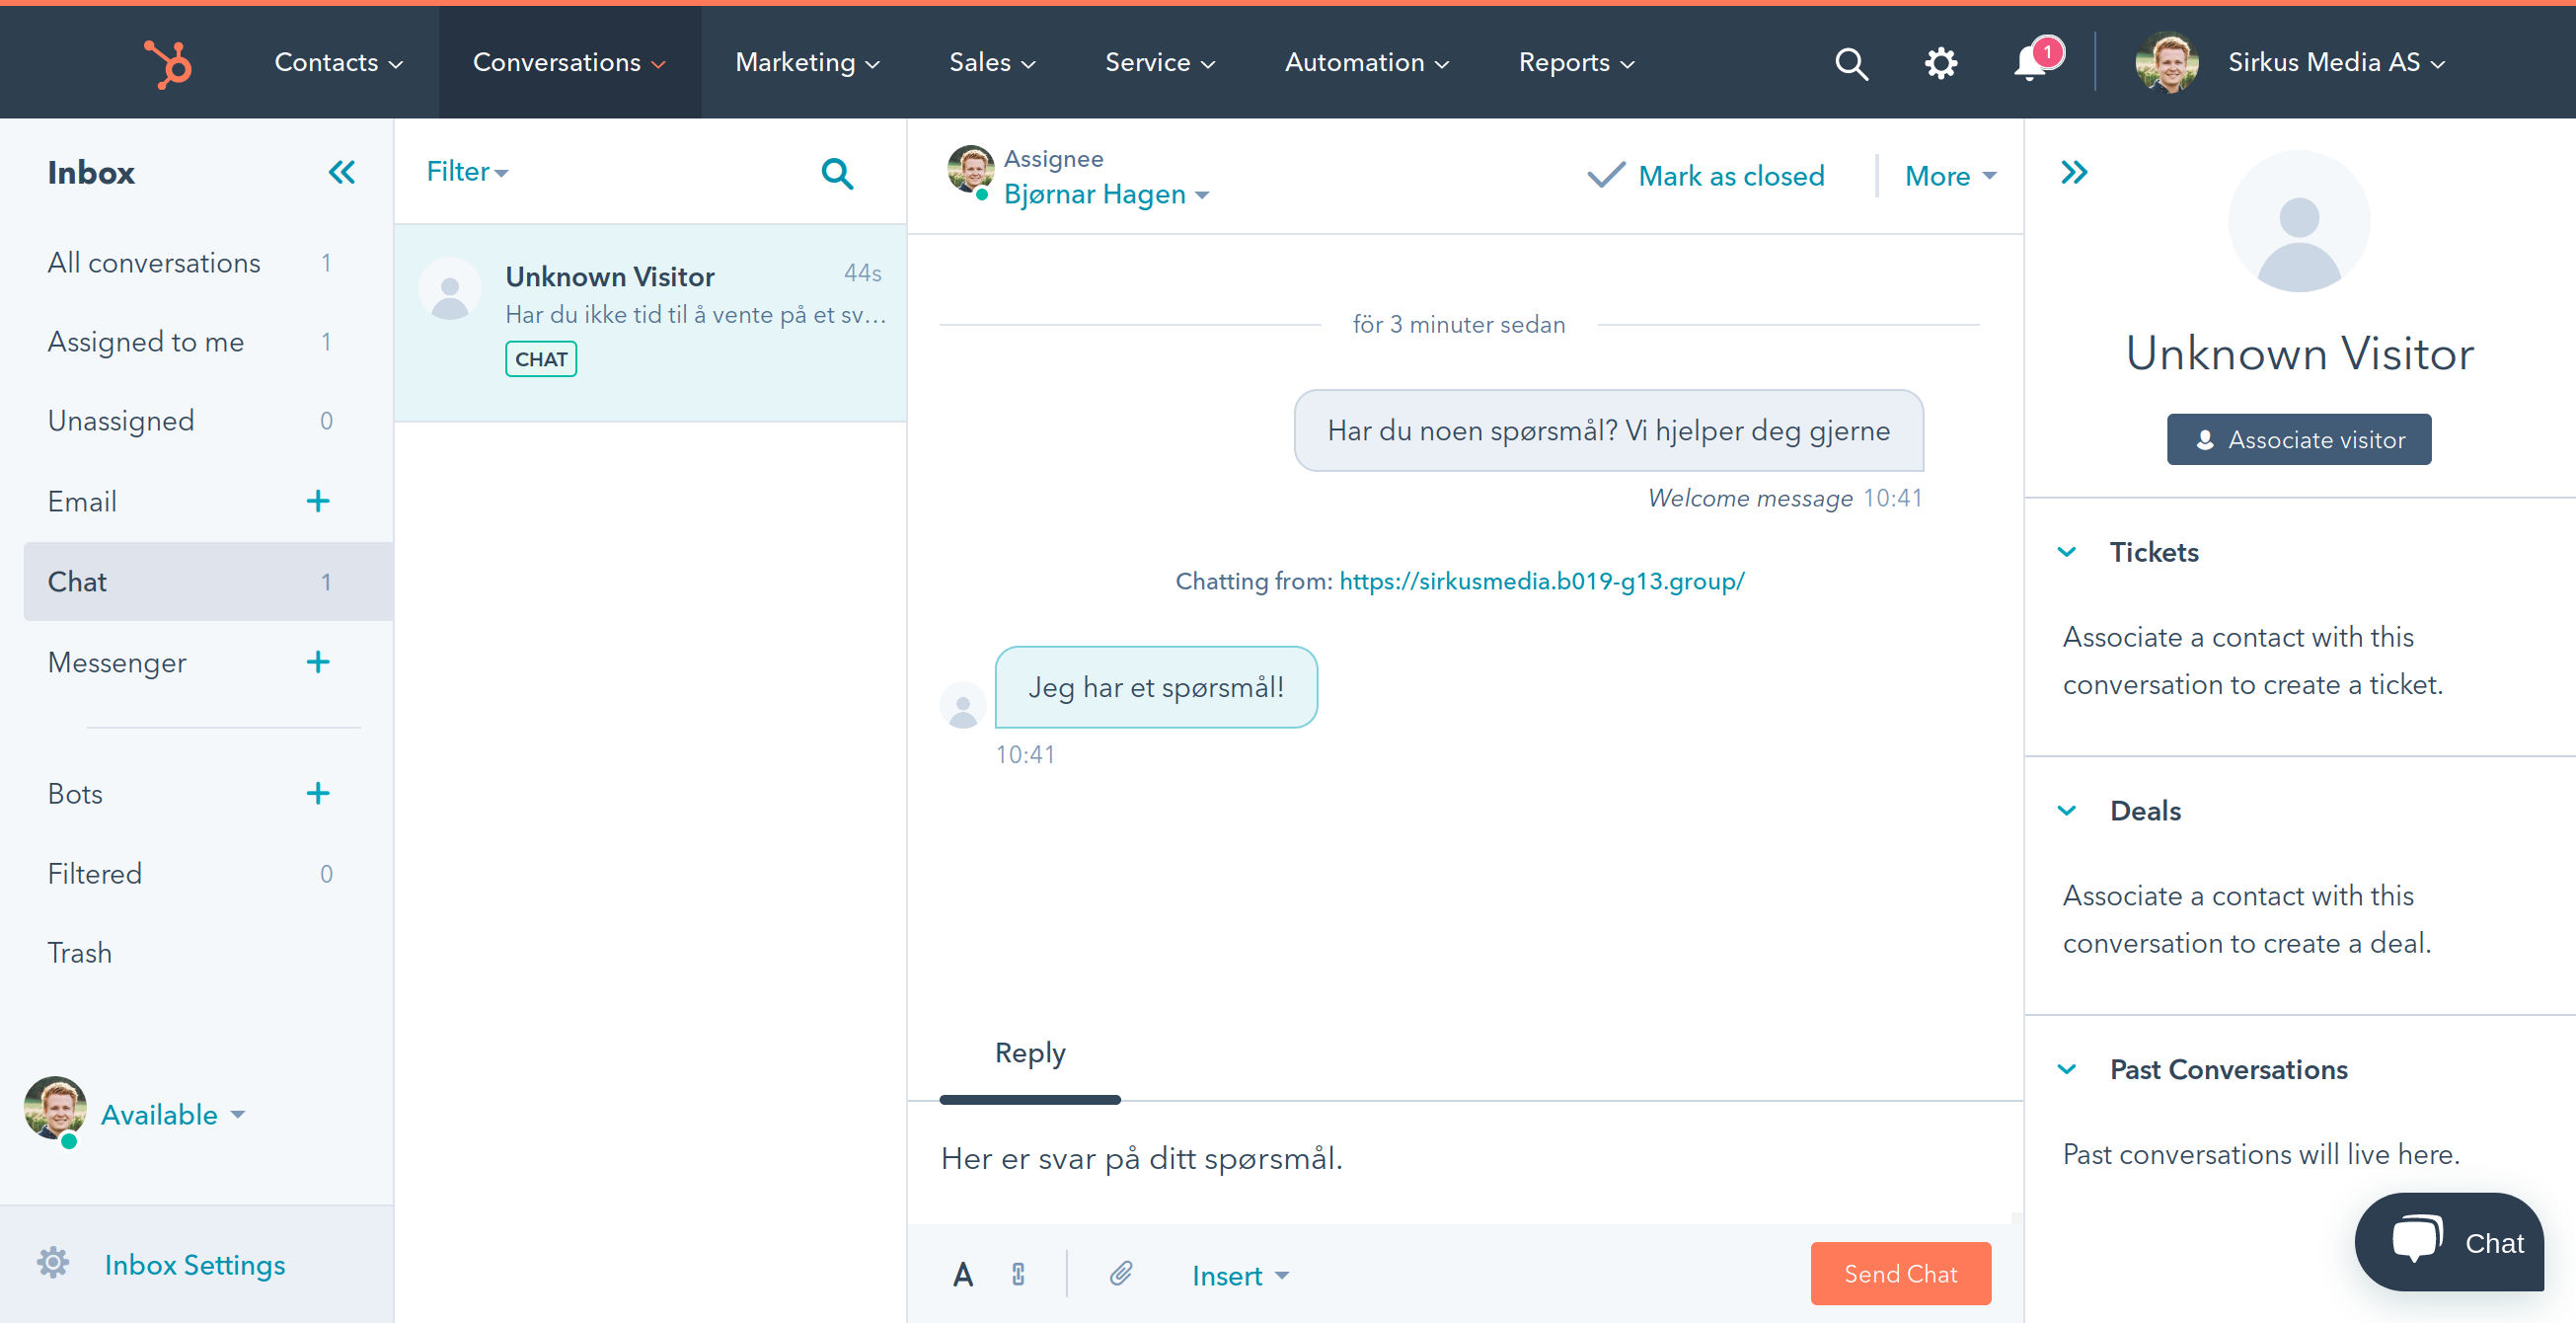
\includegraphics[width=\textwidth]{bjornar/chat-admin.png}
    \caption{Chat for admin}
    \label{fig:chat-admin}
\end{figure}

Vi ønsket at det skulle være lett for Sirkus Media å endre til en annen løsning for chat. Derfor endte vi opp med å legge til ekstra funksjonalitet i CMS'et. Det ble opprettet CRUD for innstillinger (\textit{site\_settings}), som kan hentes ut via API'et på samme måte som \textit{pages}. I innstillingene kan administrator endre hvilket script som blir brukt for chat-løsning, se figur \ref{fig:chat-setting}. Innstillingen for chat hentes ut av front-end, som bruker den til å linke opp til det scriptet som er angitt.
\begin{figure}[H]
    \centering
    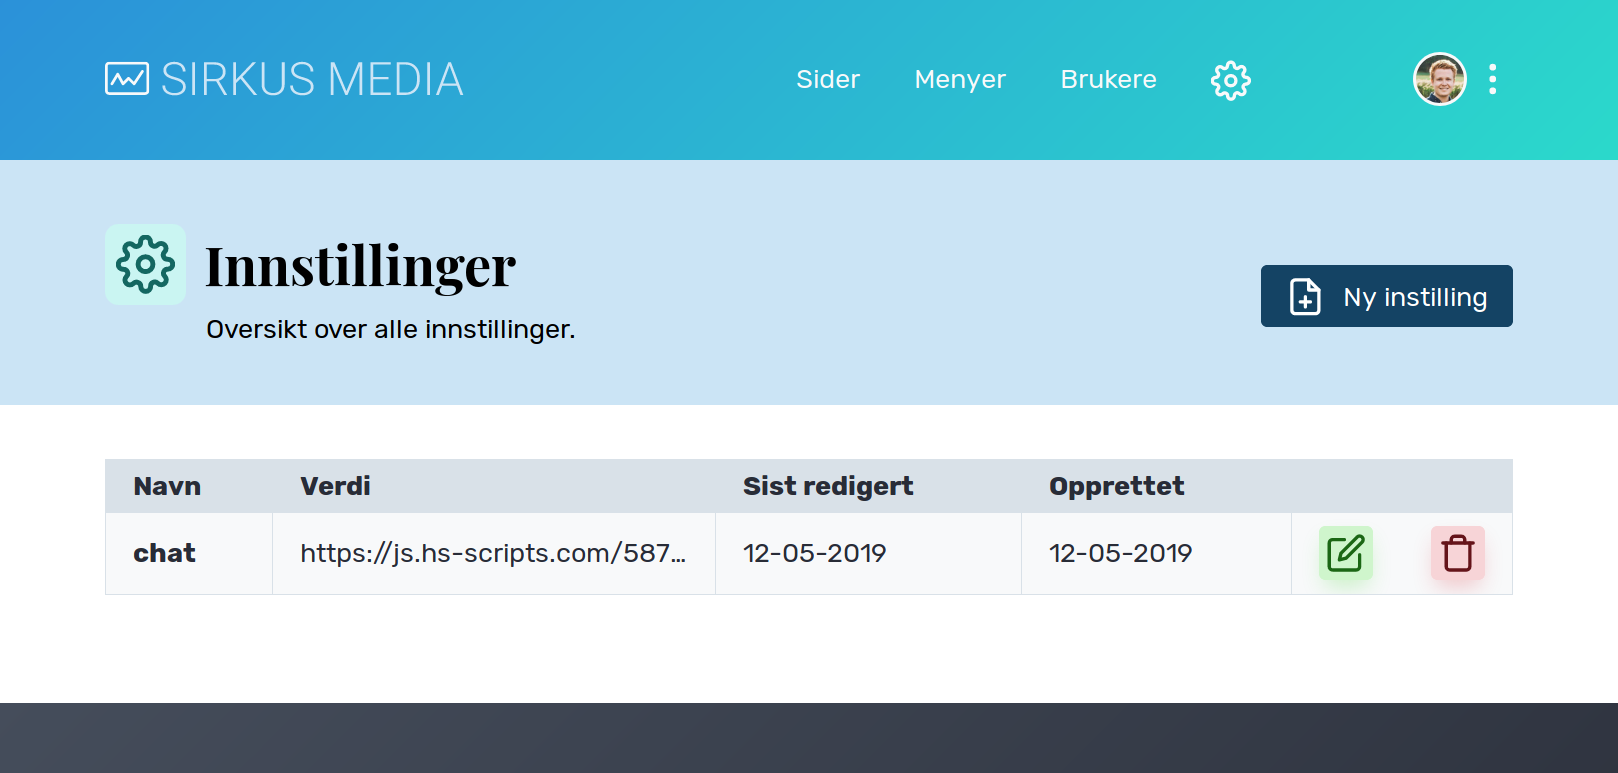
\includegraphics[width=\textwidth]{bjornar/chat-setting.png}
    \caption{Innstilling for chat i CMS}
    \label{fig:chat-setting}
\end{figure}

\section{Oppsett av kontaktskjema}
For kontaktskjema endte vi opp med en løsning fra FormSpree\footnote{\url{https://formspree.io/}}. Det eneste som trengs for å ta i bruk denne, er å sette \textit{action} på kontaktskjema til en URL som dette: \url{https://formspree.io/navn@domene.no}. Hvilken \textit{action} som brukes av kontaktskjema kan styres gjennom CMS'et.

\section{Front-end}
\subsection{Oppsett av React og tilhørende verktøy}

Det første som ble gjort i denne prosessen var å laste ned Node.js\footnote{\url{https://nodejs.org/en/}}. I dette prosjektet blir ikke Node brukt som en back-end tjeneste eller server, men for å kunne kjøre alle verktøy som må til for å kunne utvikle lokalt på datamaskinen. Det var den nyeste versjonen (11.9.0) som ble lastet ned. Deretter ble nettleserutvidelsen React Developer Tools lagt til fra  webstoren til Google Chrome. Det ble også opprettet et repository på Github og lastet ned på maskinen ved hjelp av GitKraken. 
Videre var det nødvendig med et kommandolinjevindu og en teksteditor, valget falt da på kommandolinjevinduet Powershell og teksteditoren Visual Studio Code.

For å sette opp selve React, ble  guiden til react.org for å sette opp en ny React App\footnote{\url{https://reactjs.org/docs/create-a-new-react-app.html\#create-react-app}} fulgt. Her ble det oppgitt at følgende kommandoer må kjøres for å opprette et nytt prosjekt:
\begin{lstlisting}[caption={Oppretting av React App},language=bash]
npx create-react-app my-app
cd my-app
npm start
\end{lstlisting}

Det oppstod problemer når kommandoen \q{npx create-react-app my-app} skulle kjøres, og det kom flere og lange feilmeldinger. Dette måtte undersøkes nærmere, og etter et Google-søk på deler av feilmeldingen ble det oppdaget en sak på Github som omhandlet samme problem\footnote{\url{https://github.com/facebook/react/issues/11933}}.
Løsningen var å installere yarn og create-react-app globalt med yarn. Vi la så til følgende i windows PATH, så kommandoen kunne kjøres:
\begin{lstlisting}
C:\\Users\Line Sharina\AppData\Local\Yarn\bin
\end{lstlisting}
Dette løste problemet og prosessen kunne fortsette. Da ble følgende gjort:

\begin{itemize}
    \item Kjørte \q{npm install} i mappen for prosjektet.
    \item Kjørte \q{npm start} for å starte react serveren.
\end{itemize}

Etter disse stegene begynte planleggingen av de forskjellige komponentene.

\subsection{Planlegging av komponenter}
Komponenter i React kan beskrives som gjenbrukbare biter av kode. En stor fordel med komponenter er at de er mulig å gjenbruke, slik at det ikke lenger er nødvendig å skrive den samme koden flere ganger. 

Ved å se på den godkjente mockupen ble følgende komponenter fastsatt: 
\begin{itemize}
    \item Meny
    \item Header
    \item Resultater
    \item Prosess
    \item Steg i prosess
    \item Kontaktskjema
    \item Footer
    \item Ikon + link
    \item Ikon + tekst
    \item Hvit boks under header. ActionBox
    \item Actions til actionsbox
\end{itemize}

\subsection{Oppretting av components}
Prosessen med oppretting av komponenter startet med å lage en samlemappe som ble kalt \q{components}, som ligger i mappen src. For hver komponent ble det laget en ny undermappe som inneholdt koden til selve komponenten og eventuelt tilhørende stilark.

\subsection{Ruting (Routing)}
Ruting er et mønstergjenkjenningssystem som tar seg av innkommende forespørsler og sender de til spesifikke kontroller-funksjoner. Ruting er ikke innebygd i React. Det ble derfor laget en Router.js-fil i components-mappa. Etter dette ble følgende kommando kjørt:

\begin{lstlisting}[caption={Installering av React ruting},language=bash]
npm install react-router-dom
\end{lstlisting}

Deretter kunne vi importere react-router-dom i filen Router.js:

\begin{lstlisting}[caption={Importering av react-router-dom},language=bash]
import {BrowserRouter, Route, Switch} from "react-router-dom";
\end{lstlisting}

Den foreløpige versjonen av back-end ble lastet ned og lagret lokalt, slik at det ble mulig å teste underveis.

For å kunne snakke og bruke foreløpig backend ble Axios\footnote{Se mer i avsnitt \ref{sec:tool:axios}} benyttet. Hvis etableringen av forbindelsen er vellykket, slik at det har blitt opprettet kontakt med API via Axios, vil alle svar som ble gitt av back-end bli lagret i en array. 

Deretter ble det satt opp en dynamisk ruting, ved hjelp av en løkke som går igjennom alle eksisterende sider og setter opp linker til disse.

\subsection{Installering av Axios}
Axios blir i vårt system brukt til å sende forespørsler til back-end. Dette biblioteket ble installert ved å kjøre kommandoen under.  Kommandolinjevindu må åpnes i filstilen der mappa til prosjektet er plassert.
\begin{lstlisting}[caption={Installering av Axios},language=bash]
npm install axios
\end{lstlisting}

\subsection{Page components}

Det ble opprettet et objekt som inneholder alle komponentene som er definert i databasen. Ved å loope igjennom alle komponentene til en side, ble det da mulig å sjekke om navnene samsvarte. Hvis de gjør dette, vil det kjøres en løkke som går igjennom alle feltene en komponent inneholder. Til slutt blir alle komponentene til en side, med riktige props\footnote{Props i React brukes til å sende med utvalgt data til en komponent} skrevet ut.  

Før det ble opprettet et objekt som inneholdt alle eksisterende components, ble det forsøkt å kun hente ut angitt komponenter til siden i back-end og så opprette components ut av dette. Da fikk vi følgende feil:
\begin{lstlisting}
<HeaderComponent /> is using incorrect casing. Use PascalCase for React components, or lowercase for HTML elements.
\end{lstlisting}

Feilmeldingen var at komponenten brukte feil casing, noe som ikke var riktig da feilmeldingen viste at \q{\textless HeaderComponent /\textgreater} var skrevet på riktig måte. Etter en del feilsøking, fant vi ingen som hadde løst dette problemet tidligere. Vi endte derfor opp med å opprette objektet som inneholder alle komponentene. 

I tillegg til å finne ut av hvilke komponenter som tilhører siden, må man i tillegg finne ut av hvilke felter som tilhører hvilke komponenter. Dette blir satt i back-end. I løkka som går igjennom objektene ble det derfor lagt til en ny løkke, som går igjennom og lagrer alle tilhørende felter til en komponent i en array. Denne arrayen blir så sendt videre som props i de ulike komponentene.

\subsection{Child components}
I systemet vårt kan en komponent ha flere \q{barn}. Det å ha komponenter som er barn av en komponent gjør at disse har et forhold til hverandre. Da blir det mulig å putte forskjellig innhold inn i en felles seksjon.

\subsection{Felter med samme navn}
Underveis i prosessen ble det oppdaget at hvis en komponent hadde den samme felttypen flere ganger, ville bare den siste verdien bli skrevet ut. En komponent vil ofte bestå av for eksempel flere tekstfelt, og derfor måtte vi finne en måte å løse dette på.

Løsningen ble en betingelsetest der det blir sjekket om samme felttype er til stede flere ganger. Hvis denne blir sann, vil feltene med verdier bli lagt til i en array. 

\subsection{Utskrift av tomme felter}
Videre i prosessen ble det oppdaget at hvis en prop ikke innholdt en verdi, ville feltet fortsatt bli skrevet ut. Dette førte til at nettstedet inneholdt mange tomme HTML-tagger. Brukervennligheten på for eksempel skjermlesere hadde blitt betraktelig dårligere, så derfor måtte dette gjøres om. Løsningen ble å gjøre en betingelse-test på hver prop, for å sjekke om den innholdt en verdi. Da ble det mulig å kun skrive ut om dette var oppfylt.

\subsection{Testing}
For å teste systemet, ble header-komponenten laget. Når denne ble opprettet både i objektet og back-end, ble alle props/feltene som blir mottatt fra komponenten skrevet ut. Dette betydde at Header-komponenten fungerte som den skulle, og vi kunne starte med å legge til resten av komponentene på samme måte. 

Da kunne vi også begynne å style komponentene slik at de ligner mockupen som ble laget.

\subsection{Kompilere SCSS til CSS}
Gruppen har tidligere nevnt at det ble besluttet å bruke SASS til styling. Da er det nødvendig å ha noe som kompilerer fra SCSS til CSS. Dette ble oppnådd ved å følge guiden hos TechCookbook\footnote{\url{https://techcookbook.com/react/use-scss-with-create-react-app}}

Installerte først node-sass ved å kjøre :

\begin{lstlisting}[caption={Installering av node-sass},language=bash]
npm install --save node-sass
\end{lstlisting}

Etter at pakken ble installert, måtte det lages et script som kompilerer fra .scss til .css:

\begin{lstlisting}[caption={Kompliering fra .scss til .css}]
 "build-css": "node-sass src/ -o src/"
\end{lstlisting}
\clearpage

\q{Build-css} tar .scss-filene som finnes i source-mappen samt undermapper og kompilerer dem til .css-filer. .css filen vil bli tilgjengelig i den samme lokasjonen som den originale .scss-filen. Deretter ble det laget et script som kjører \q{build-css} og kompilerer alle eksisterende filer til .css, samtidig som den ser etter forandringer i source-mappen. Den vil altså detektere om det blir gjort endringer i eksisterende .scss filer, eller om det blir lagt til nye. 

\begin{lstlisting}[caption={Script som detekterer scss endringer}]
 "watch-css": "npm run build-css && node-sass src/ -o src/ --watch --recursive"
\end{lstlisting}

En test ble gjort ved å lage en fil som het "header.scss" og satte bakgrunnsfargen til rød. Dette fungerte som det skulle.

\begin{lstlisting}
 body {
  background-color: red;
}
\end{lstlisting}

\subsection{Styling}
Designet til nettstedet ble stylet ved hjelp av SCSS, og er så lik den godkjente mockupen som mulig. Designet er også responsivt og fungerer derfor like godt på stor skjerm, laptop, nettbrett og mobil. For stylingen ble prinsippet \q{mobil først} benyttet. Dette prinsippet går ut på at utviklingen først skjer for små skjermer, for deretter å skalere opp og gjøre designendringer når det er nødvendig. 

\subsection{Ikoner og illustrasjoner}
Ikonene er hentet fra Feather\footnote{\url{https://feathericons.com/}}. Feather er en ikonpakke med åpen kildekode. Alle illustrasjonene er hentet fra unDraw\footnote{\url{https://undraw.co/}}. På nettsiden til unDraw oppgir de at både private og kommersielle kan bruke og modifisere illustrasjonene gratis\footnote{\url{https://undraw.co/license}}. Siden disse er av filtypen SVG har vi hatt muligheten til å tilpasse fargene på illustrasjonene til å passe designet til nettstedet.

\section{DevOps}
Vi har ikke fått all informasjon som skal på nettstedet eller tilgang til domenet til Sirkus Media. Nettsted og CMS måtte derfor lastes opp på midlertidig domener.
I forbindelse med prosjektet skulle gruppen ha et eget nettsted der det er informasjon om oppgaven og gruppen, samt oppdatering underveis i prosessen. Det ble derfor kjøpt et eget domenet for dette: \url{b019-g13.group}. Vi bestemte oss for å bruke det samme domenet. Det ble opprettet et subdomene hver for front-end og back-end: \url{sirkusmedia.b019-g13.group} og \url{api.b019-g13.group}.

Front-end ble lastet opp og kan styres via Netlify\footnote{\url{https://www.netlify.com/}}. Back-end skulle i utgangspunktet settes opp på en virtuell server hos DigitalOcean\footnote{\url{https://www.digitalocean.com/}}, som vi selv satt opp med LEMP. Vi endte opp med en litt annen løsning, der alt settes opp og styres gjennom Laravel Forge\footnote{https://forge.laravel.com/} og oppdateres med Envoyer\footnote{\url{https://envoyer.io/}}. Oppsettet kjører forsatt på en VPS hos DigitalOcean, men vi trengte ikke lenger å sette opp LEMP.

\section{Første versjon av database, CMS og nettsted}
Det ble noen avvik fra den planlagte databasen. Databasen ble derfor mer optimalisert og bedre tilpasset det oppsettet vi ønsket, se figur \ref{fig:first-version-db} og \ref{fig:first-version-db-other}.

\begin{figure}[H]
    \centering
    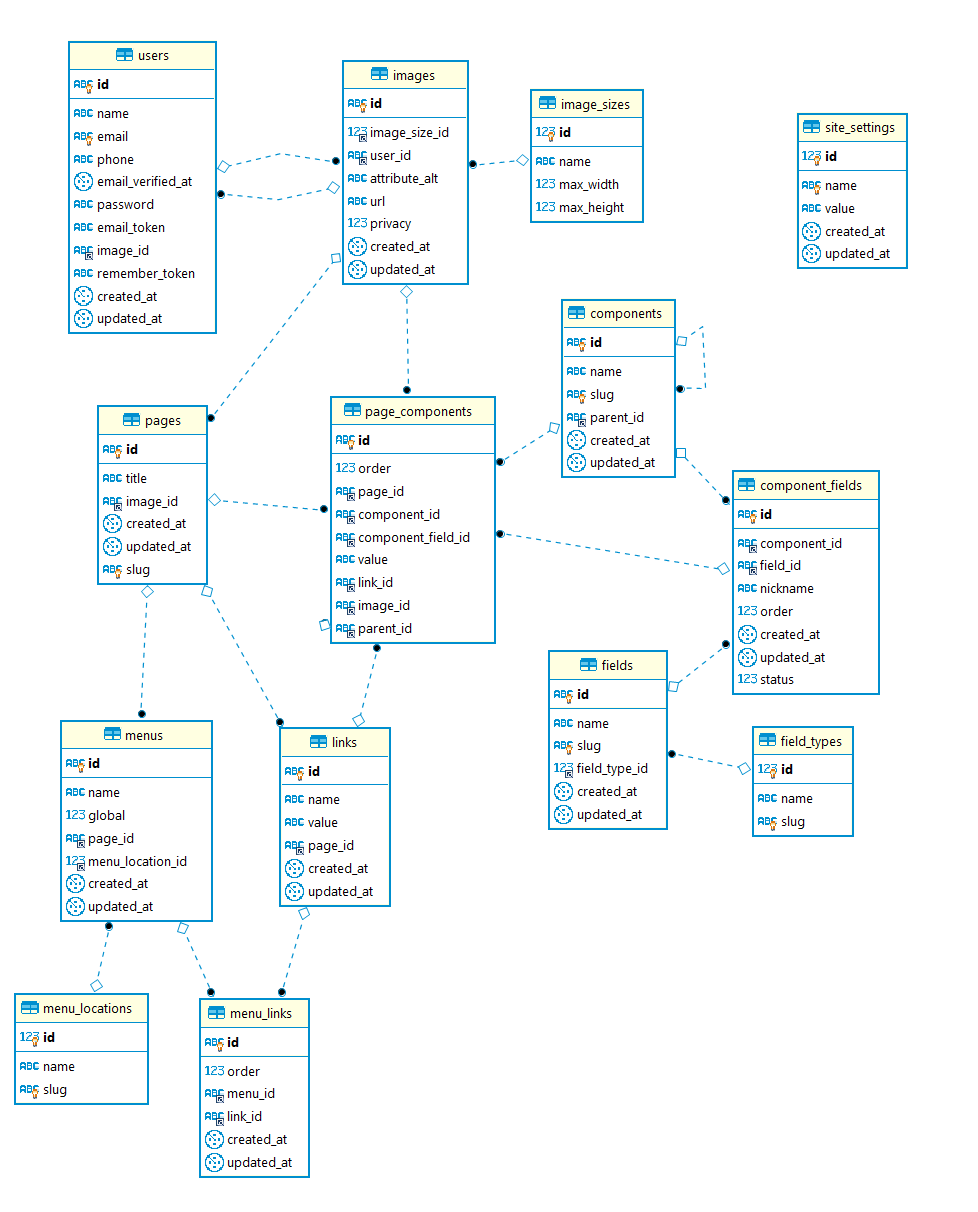
\includegraphics[width=\textwidth]{bjornar/db-endelig.png}
    \caption{Første versjon av databasen - hovedtabeller}
    \label{fig:first-version-db}
\end{figure}

\begin{figure}[H]
    \centering
    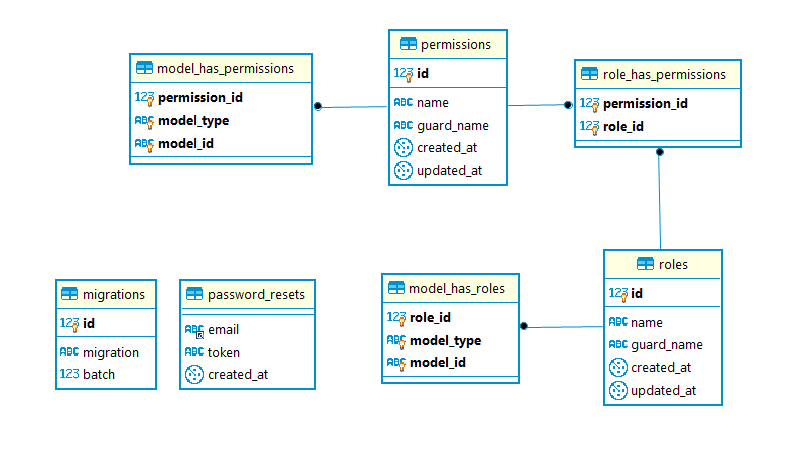
\includegraphics[width=\textwidth]{bjornar/db-endelig-annet.png}
    \caption{Første versjon av databasen - andre tabeller}
    \label{fig:first-version-db-other}
\end{figure}

CMS-et endte opp med å bli som vi planla i avsnitt \ref{sec-planning-cms}. Det var kun en ekstra funksjonalitet som ble lagt til, muligheten til å gi kallenavn til felter som tilhører komponenter. Dette gjør det enklere for sluttbruker å redigere sider. En funksjonalitet som ble diskutert under planlegging, men aldri skrevet ned var en bildevelger. Felter som er av typen bilde, har en referanse til Image-modellen. For å sette verdien til dette feltet på riktig måte, trenger man en ID til et bilde i \q{images}-tabellen. Alt dette tar bildevelgeren seg av, samt at den gjør det enkelt å laste opp nye bilder. Figur \ref{fig:first-version-cms} viser første versjon av CMS-et, og \ref{fig:media-picker-cms} viser bildevelgeren til CMS-et.

\begin{figure}[H]
    \centering
    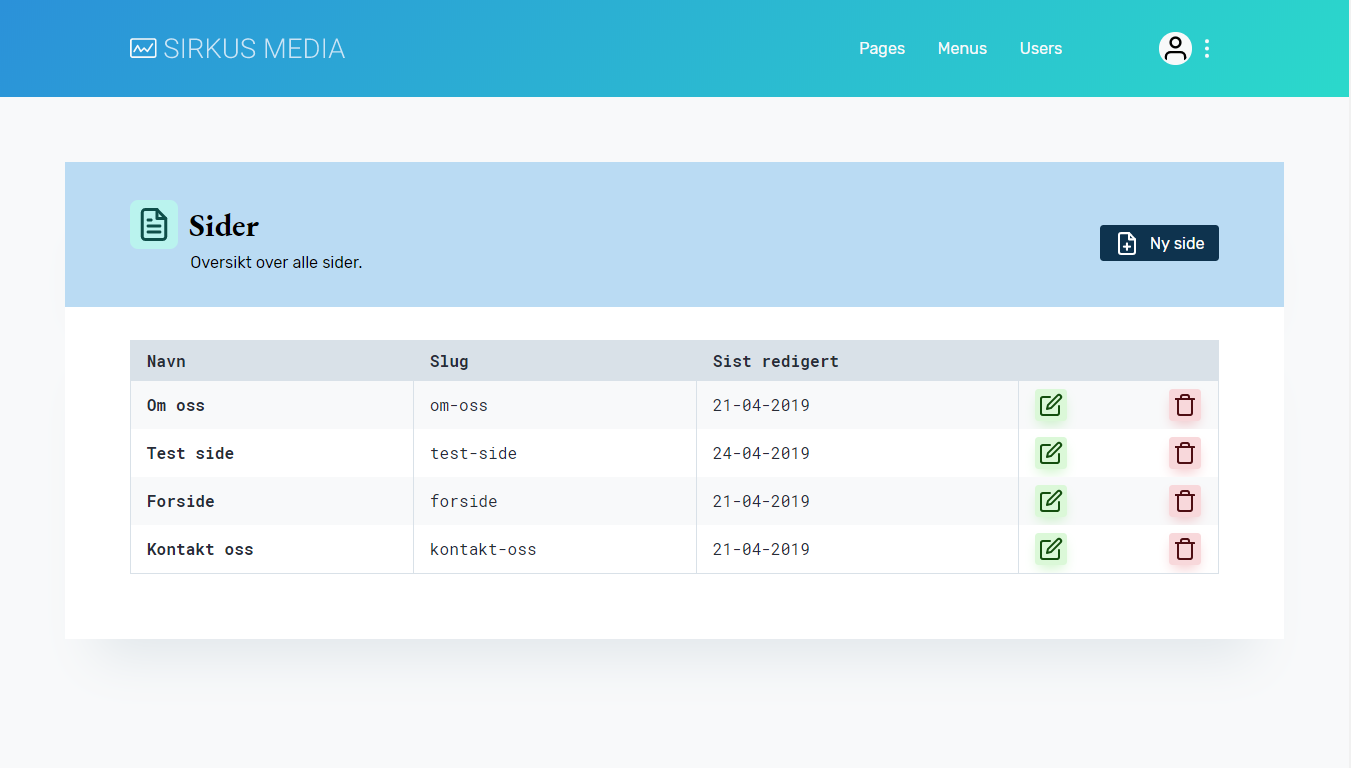
\includegraphics[width=\textwidth]{first-version-cms.png}
    \caption{Første versjon av CMS-et}
    \label{fig:first-version-cms}
\end{figure}

\begin{figure}[H]
    \centering
    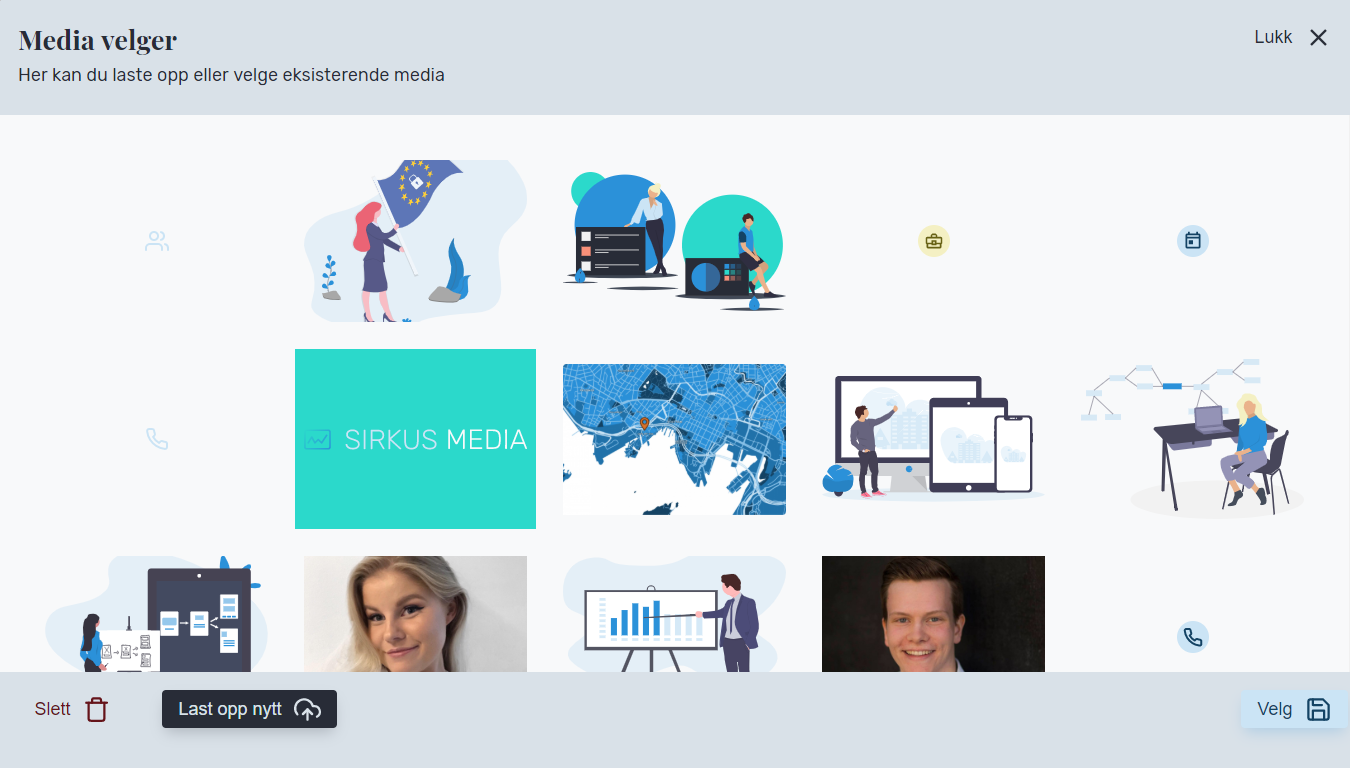
\includegraphics[width=\textwidth]{brukerveiledning/media-picker.png}
    \caption{Bildevelgeren til CMS-et}
    \label{fig:media-picker-cms}
\end{figure}

Nettstedet endte også opp som vi planla i avsnitt \ref{sec:planning-website}. Både forsiden, menyen, om- og kontakt oss siden ble utviklet uten avvik. Videre innholder footeren en link som fører til logg inn til administrasjonsgrensesnittet. Det har også blitt opprettet sider for personvern og informasjonskapsler. Disse innholder tekst fra den opprinnelige nettsiden til oppdragsgiver. Nettstedet består i tillegg av en chat, der meldingene blir sendt direkte til en e-postadresse. Figur \ref{fig:first-version-website} viser første versjon av nettstedet.

\begin{figure}[H]
    \centering
    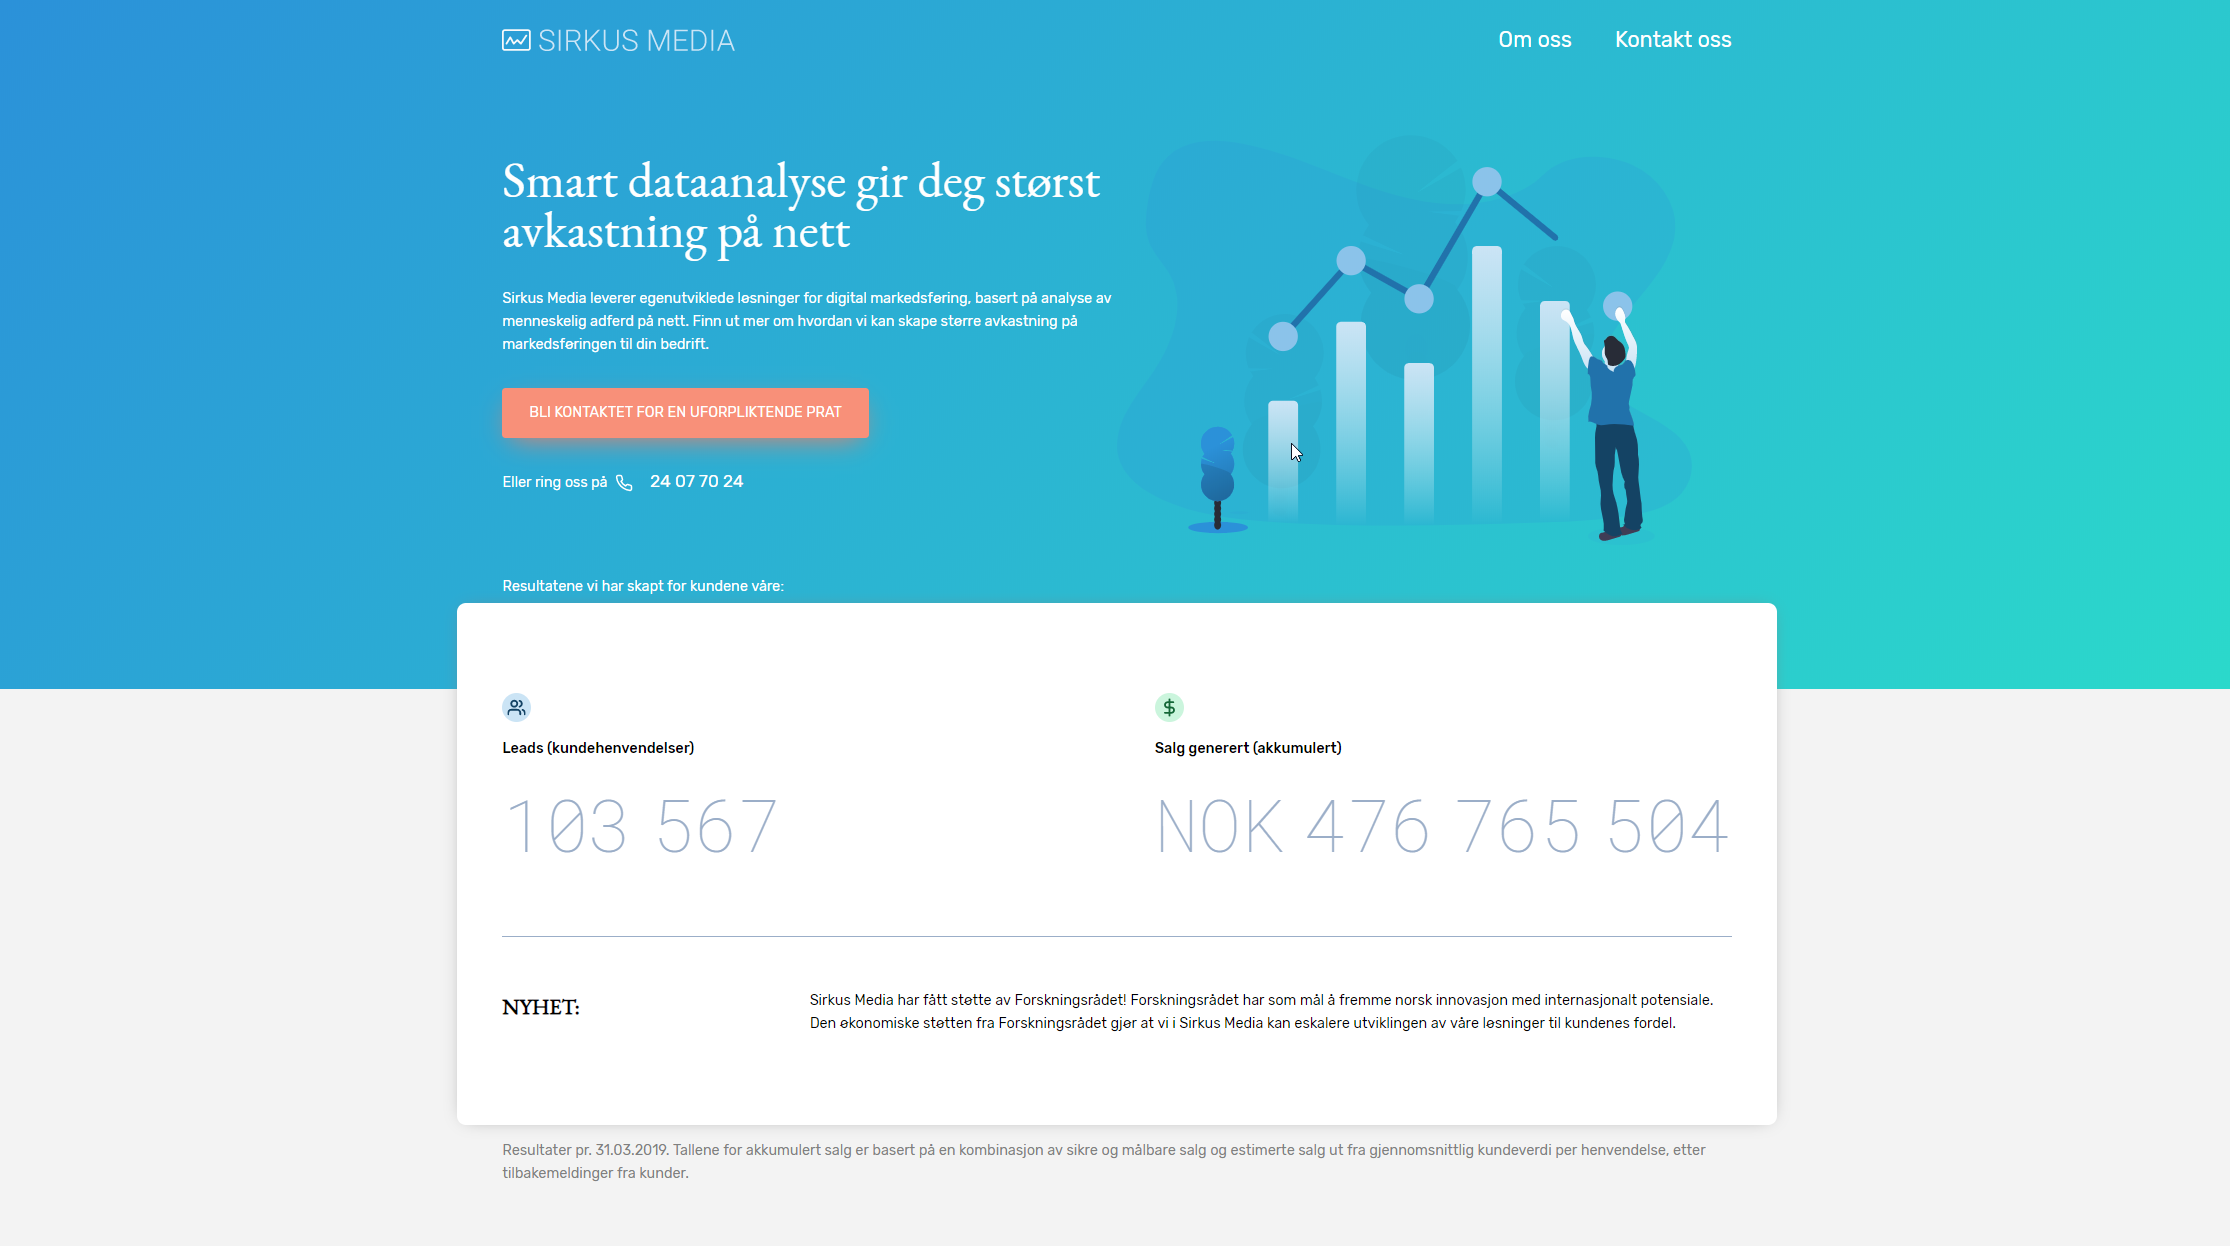
\includegraphics[width=\textwidth]{versjon-1-nettsted.png}
    \caption{Første versjon av nettstedet}
    \label{fig:first-version-website}
\end{figure}
    \cleardoublepage
\chapter{Test av CMS og nettsted}
\label{chap:evaluation} 
% \meta{
% De fleste prosjekter avsluttes med en eller annen form for evaluering av resultatene fra prosjektene. I utviklingsprosjekter vil det være naturlig med teknisk testing, fungerer programvaren som den skal? Teknisk testing kan utføres av utviklerne selv, eller en ekstern part, f.eks. oppdragsgiver. En oppdragsgiver ønsker ofte å utføre en akseptansetest, dvs. en test som vil avgjøre om de har "fått det de har betalt for". Ellers vil det i mange tilfeller være nyttig og viktig med en brukertest, dvs. en strukturert test der sluttbrukerne får komme til orde.

% Evalueringsmetoden vil altså avhenge sterkt av typen av prosjekt. Likevel vil de samme overordnete prinsippene gjelde for alle typer leveranser. En utredning bør kunne passere en akseptansetest, et mediaprosjekt bør kunne underlegges både akseptanse- og brukertest (jfr. kritikerprosessen rundt nye spillefilmer), og et programvareprosjekt bør i tillegg gjennomgå en teknisk test.
% }

I dette kapittelet vil vi gjøre en evaluering av det ferdige nettstedet. Her vil resultatene fra en teknisk test, brukertest og til slutt en akseptansetest av oppdragsgiver bli presentert.

\section{Teknisk test}
I dette kapittelet vil vi gjennomføre den samme testen som ble utført i konkurrentanalysen (kapittel \ref{sec:competitor-analysis}).

\subsection{Konklusjon}

\section{Brukertest}
For å brukerteste har vi laget forskjellige caser som de forskjellige personene skal gjennomføre. Brukertesten ble gjennomført av 3 personer i ulike aldersgrupper.

\subsection{Caser}

\subsubsection{Case 1}
Du ønsker å lære mer om bedriften og visjonen bak Sirkus Media. Hva gjør du for å løse dette?

\subsubsection{Case 2}
Du ønsker å lære mer om tjenestene til Sirkus Media. Hva gjør du for å løse dette?

\subsubsection{Case 3}
Du ønsker å komme i kontakt med Sirkus Media. Hva gjør du for å løse dette?

\subsection{Testing av nettstedet}

\subsubsection{Testperson 1}
Test person 1
Kvinne 60 år

\subsubsection{Testperson 2}
Mann 50 år

\subsubsection{Testperson 3}
Testperson 3 var en kvinne 25 år som utførte testen på laptop.

\subsection{Konklusjon}


\section{Akseptansetest}
Etter at første versjonen av nettsted og CMS var ferdig, kunne oppdragsgiver teste systemet. Målet med denne testen var å kartlegge hvor fornøyd oppdragsgiver var med produktet, samt hvilke endringer som burde foretas. I akseptansetesten blir det mulig for oppdragsgiver å verifisere at leveransen er i henhold til bestillingen. 

Etter at versjon 1 ble lastet opp fikk oppdragsgiver beskjed om å teste å prøve å lage en ny side med komponenter og innhold, endre eksisterende sider og slette den nyopprettede siden. Før testingen ble det sendt ut brukerveiledning på e-post\footnote{Se vedlegg XX}. Oppdragsgiver fikk også beskjed om å gå igjennom de forskjellige sidene og komme med tilbakemelding på designet. 

\subsection{Konklusjon}

% Testingen av de to verktøyene er utført på en uformell og ikke særlig vitenskapelig basert måte, og resultatene baserer seg hovedsakelig på forfatterens egne vurderinger\footnote{I et reelt prosjekt ville denne metoden være litt for tynn \smiley}.

% I Tabell \ref{tab:comparison} er det foretatt en summarisk sammenlikning mellom OpenOffice og \LaTeX~ med hensyn på kravene i Kapittel \ref{sec:generelle-krav}.


% \begin {table}[h!]

% \begin{center}
% \begin{longtable}{|l|p{0.332\textwidth}|p{0.33\textwidth}|}
% \hline
%  {\bf Krav} & {\bf OpenOffice} & {\bf \LaTeX} \\ 
% \hline
% Robusthet & Tildels betapreget. Man har av og til følelsen av å bevege seg på  tynn is. & Bunnsolid, Gigabyte type dokumenter ingen problemer.\\ 
% \hline
% Åpne formater &
% Ja. En ODF fil er en zipfil som inneholder en rekke skjemadefinerte XML filer. &
% Ren, ``lettlest'' ASCII.\\ 
% \hline
% Maler/stiler &
% Ja, men noe rotete, lett å overstyre lokalt uten at du merker det. &
% LaTex ``oppfant'' prinsippet med å skille innhold, struktur og presentasjon. Enormt tilfang av maler og stiler for det meste.\\ 
% \hline
% Oppsplitting &
% Mulig, men ikke trivielt/robust. &
% Trivielt. Modus Operandi for store dokumenter, f.eks. Proceedings som samler ``stand-alone''-artikler fra mange forfattere.\\ 
% \hline
% Kryssreferanser &
% Går greit, men ikke helt intuitivt. &
% Konsistent og enkelt.\\ 
% \hline
% Bibliografi &
% Greit med bruk plugins/extensions, f. eks, Zotero. &
% BibTex innførte prinsippet om å referere til eksterne bibliografisamlinger. En mengde ulike stiler.\\ 
% \hline
% Brukermasse &
% Stadig økende, men med stort innslag av entusiaster og ``pionerer''. &
% Stor og kompetent, særlig innen den naturvitenskapelige og tekniske delen av akademia.\\ 
% \hline
% Dokumentasjon &
% Relativt god, men bærer preg av at produktet er ``ferskt''. &
% Meget omfattende, men godt spredt i ulike fora.\\ 
% \hline
% Versjonering &
% En odf-fil er en binærfil (zippet og komprimert samling XML-dokumenter), og egner seg dårlig for tradisjonell versjonskontroll. Det finnes en innebygget versjonerings-mekanisme, men det er usikkert hvor hensiktsmessig denne er.&
% Filene er ren ASCII, og håndteres derfor trivielt i alle typer versjoneringssystemer.\\ 
% \hline
% Framtidssikker &
% Uklart, siden det er et ``ferskt'' verktøy, men potensialet er der.&
% Kan ikke bli bedre? Egen erfaring med komplekse og store dokumenter fra tidlig 90-tall som problemløst kan  behandles i dagens verktøy.\\ 
% \hline
% Staving/grammatikk &
% Innebygget, mulig å laste inn ulike typer eksterne ordlister etc.&
% Mange vektøy, fordi filene er ren ASCII.\\ 
% \hline
% \end {longtable}
% \caption {Summarisk vurdering av sentrale aspekter i OpenOffice og \LaTeX~\label{tab:comparison} }
% \end{center}
% \end {table}






    \cleardoublepage
\chapter{Diskusjon}
\label{chap:discussion} 
% \meta{
% Diskusjonskapittelet er viktig, både for dere selv og sensor. Dette kapitellet er det som i hovedsak skiller et akademisk prosjekt fra et rent næringslivsprosjekt. Det er her dere skal dokumentere at dere har lært noe underveis, ikke bare levert et produkt til en oppdragsgiver. 
% Her går dere tilbake til Avsnitt \ref{sec:maal-metode-resultater}. I hvilken grad ble målene oppnådd
%  (Avsnitt \ref{sec:maal})? Leverte dere de forventede resultatene (Avsnitt \ref{sec:resultater})? Fungerte metoden
%  dere beskrev i  Avsnitt \ref{sec:metode}?
% Hva ble bra? Hva ble ikke fullt så bra? I begge tilfeller, hvorfor? Hva slags problemer støtte dere på? Hva ville dere gjort anderledes, sett i ettertid? 
% }

I dette kapittelet vil vi se på om metoden vi beskrev i introduksjonen fungerte og om målene som ble satt i starten av prosjektet har blitt oppnådd. Vi skal også se på om forventet resultat ble levert. I tillegg skal vi presentere hva som har gått bra, hva som har gått mindre bra og hva slags problemer som har oppstått underveis. Til slutt gjør vi en utredning på hva som burde ha blitt gjort annerledes, sett i ettertid.

\section{Ble målene oppnådd?}
I avsnitt \ref{sec:maal} definerte vi noen mål for prosjektperioden. Disse var som følger:

\begin{compactitem}
\item [{\bf Hovedmål}] Forbedre profilen til Sirkus Media på nett, slik at potensielle kunder får en bedre forståelse av deres produkter og tjenester og dermed tar kontakt gjennom nettstedet. På et overordnet plan vil dette bidra til å øke omsetningen til oppdragsgiver.
\begin{compactitem}
\item [{\bf  Delmål 1} ] Generere mer trafikk, som fører til at flere kunder tar kontakt med bedriften. 
\item [{\bf  Delmål 2} ] Måle trafikken på nettstedet, slik at man ser hva som fungerer og deretter kan tilpasse informasjonen til brukerne som besøker siden.
\end{compactitem}
\end{compactitem}

Vi ser i ettertid at det ikke er mulig for oss å sjekke at delmålene har blitt oppfylt før etter endt bachelor, og de burde derfor blitt definert annerledes. Eventuelt burde vi ha lastet opp nettstedet tidligere, slik at vi hadde fått lengre tid til å analysere trafikken. Planen var å benytte oss av verktøyet Google Analytics for å måle både trafikken og observere hvordan brukere benytter nettstedet. Dette fikk vi dessverre ikke tid til, og vi vet derfor ikke om delmål 1 er oppfylt. Delmål 2 er ikke oppfylt, da vi ikke har satt opp noe verktøy for måling på nettstedet.

Når det kommer til hovedmålet vil vi likevel påstå at det er oppfylt. Vår løsning er mer innbydende, har et moderne utseende og gjenspeiler visjonen og bedriften bedre enn den tidligere løsningen. Vi har også en bedre presentasjon av bedriften, prosessen og deres tjenester som gjør det lettere for kundene å forstå hva oppdragsgiver tilbyr. Det er også lettere å ta kontakt gjennom det nye nettstedet, da kontaktskjemaet befinner seg flere steder, live-chatten er tilgjengelig på alle sider og både e-postadresse og telefonnummer til bedriften ligger lett tilgjengelig. Disse punktene tror vi kommer til å bidra til at flere tar kontakt gjennom nettstedet. 

I tillegg viser resultatet fra brukertestene at informasjonen om bedriften ligger lett tilgjengelig på nettsiden, og brukerne sitter derfor lettere igjen med en god forståelse av bedriften. Samtidig klarte alle testpersonen å kontakte bedriften gjennom en av de mulige måtene på nettstedet. Vi konkluderer derfor med at hovedmålet er oppfylt. 


\section{Fungerte metoden vi valgte}
I avsnitt \ref{sec:metode} beskrev vi metoden vi hadde valgt. Etter fullført prosjektperiode, vet vi at alle analysene og planlegging vi gjorde i starten av prosjektet fungerte bra. Dette ga oss et godt grunnlag for prosjektet, da vi fikk en oversikt over oppbyggingen til CMS-et og hvordan nettstedet burde se ut. 

For å oppnå delmålet om å generere mer trafikk til nettstedet, skulle vi ha stort fokus på SEO, semantikk og universell utforming. Dette har vi hatt under hele prosessen. Problemet er at vi ikke har lagt til verktøy som måler trafikk, og vi kan derfor ikke vite om denne metoden fungerte. Videre fungerte mockups og databaser bra, da det er lettere å utvikle når du vet hvordan database og design ser ut. Likevel ble ingen av delmålene ble oppfylt, og vi kan konkludere med at vår utvalgte metode ikke fungerte optimalt.

\section{Prosjektets resultat}
Resultatet til prosjektet endte opp med å bli både et headless CMS og nettsted, og vi føler derfor at vi har levert utover forventet resultatet. Oppgaven gikk i hovedsak ut på å utvikle et nettsted, men vi har endt opp med å utvikle et eget headless CMS i tillegg til selve nettstedet. Vi ønsket å utfordre oss selv og sørge for at alle gruppemedlemmene fikk nok å gjøre, derfor ble oppgaven såpass stor. I tillegg har vi lagt stor vekt på at både CMS-et og nettsiden er responsivt, brukervennlig og at de følger beste praksiser nevnt i kapittel \ref{chap:analysis}. Videre har vi sørget for at nettstedet får gode resultater i de forskjellige testene vi har utført.

Planen var at vi skulle utvikle en visuell profil med både protype og designsystem. Vi skjønte etterhvert at vi ikke kom til å rekke alt vi hadde nevnt i leveransen, og valgte derfor å gå bort fra dette siden det ble ansett som det minst viktige. Utover dette har vi kommet i mål med alle leveransene som ble nevnt i forprosjektrapporten. Sitemap og brukerveiledning ligger vedlagt. Analyse av gammelt nettsted, konkurrent- og verktøyanalysen befinner seg i kapittel \ref{chap:analysis}. Mockups ligger i kapittel \ref{chap:design}, mens analysen av nytt nettsted befinner seg i kapittel \ref{chap:evaluation}. Videre ligger nettstedet og databaser med modeller/tabeller vedlagt på minnepenn.

\section{Det som ble bra}
Samtlige i gruppen er stolte over det ferdige produktet, og mener at resultatet både for CMS og nettstedet ble bra. Det er flere grunner til dette. Først og fremst syns vi syns at designet og brukervennligheten er god for back- og front-end. Resultatene fra brukertestene er med på å støtte vår påstand om at brukervennligheten for nettstedet er god. I brukertestene fikk vi også tilbakemeldinger på designet til nettstedet, som er med å støtter vårt utsagn om at designet er bra. I tillegg syns vi det meste av funksjonaliteten vi har lagt til i CMS-et er gjennomført og intuitivt. Vi har også fulgt best praksis på de områdene vi presenterte i kapittel \ref{chap:analysis}. Videre legger vi til rette for lover som universell utforming og GDPR. 

De tekniske testene viser at nettstedet presterer godt når det kommer til ytelse, universell utforming og SEO. Dette er andre faktorer som bidrar positivt.

Alle de foregående punktene viser hvorfor vi i studentgruppen syns det ferdige produktet ble bra.

\section{Det som ble mindre bra}
I CMS-et er vi mindre fornøyd med noe av funksjonaliteten. Det første er at om en komponent som har blitt brukt flere steder skal oppdateres, må den oppdateres på alle sidene. Hvis for eksempel footeren skal oppdateres i dag, må den oppdateres på alle sider denne komponenten er på. Footeren skal i utgangspunktet være lik på alle sider, og det kan derfor føles unødvendig å måtte oppdatere alle. Av den grunn burde denne funksjonaliteten legges til.

Videre fungerer ikke systemet helt optimalt når en link opprettes. Når en ny link har blitt lagt til, vil den ikke vises med en gang. Brukeren må oppdatere siden før den nye linken vises.

\section{Problemer vi har støtt på}
Det har oppstått problemer i utviklingsprosessen for både CMS-et og nettstedet. Disse blir beskrevet nærmere i kapittel \ref{chap:implementation}.  Mot slutten av prosessen oppdaget vi at nettsiden ikke fungerte i Internet Explorer (IE). Grunnen til dette er at IE ikke støtter biblioteket Axios, som vi har benyttet til API. Vi hadde fra før testet nettstedet i Edge, og antok da at det også kom til å fungere i IE. Dette stemte dessverrre ikke.

\section{Dette burde ha blitt gjort annerledes}
Hvis vi skulle gjennomført dette prosjektet på nytt, hadde vi utarbeidet en mer realistisk prosjektplan. Vi hadde også fulgt denne planen tettere. I tillegg hadde vi sørget for å oppdatere planen, når leveransene ikke ble ferdig til tiden vi hadde planlagt.

Som nevnt tidligere endte vi opp med å gjøre mye mer enn det oppdraget tilsa, og burde derfor vært flinkere til å begrense oss når det gjaldt tidsbruken av utvikling av brukergrensesnittet. Vi fant hele veien funksjonalitet vi ønsket å legge til for å forbedre brukeropplevelsen og som ikke nødvendigvis var en del av oppgaven vi fikk i utgangspunktet. 

Vi burde også startet å teste nettstedet i andre nettlesere tidligere, slik at vi hadde hatt bedre tid til å feilsøke og rette feilen i Internet Explorer.

Det viktigste elementet vi hadde gjort annerledes hadde vært å laste opp nettstedet tidligere, slik at vi hadde fått oppfylt delmålene. 

    \cleardoublepage
\chapter{Konklusjon}
\label{chap:conclusion} 

I dette kapittelet vil vi ta for oss hvordan det ferdige produktet ble i forhold til forventningene til oppdragsgiver og våre egne.  Vi skal også presentere hva som burde bli gjort ved en eventuell videreføring av prosjektet, og komme med råd til videre arbeid.

\section{Forventninger og det endelige resultatet}
Prosjektets hovedmål var å lage et nettsted som forbedrer profilen til Sirkus Media på nett, slik at besøkende fikk en bedre forståelse av bedriften og dermed øke sjansen for at de tar kontakt gjennom nettstedet. Dette føler samtlige på gruppen at vi har fått til. Som nevnt ved flere anledninger, føler vi at nettstedet nå fremstår som mer imøtekommende og profesjonelt, i tillegg til at det er responsivt og raskt.

Tilbakemeldingene på brukertestene var også veldig positive. Etter å ha rettet opp de punktene som fungerte mindre bra, tror vi at tilbakemeldingene hadde vært utelukkende positive om vi hadde gjort testene på nytt. 

De tekniske testene og sammenligningen av det nye og gamle systemet viser at det nye nettstedet presterer bedre med tanke på ytelse og hastighet, universell utforming, SEO og beste praksiser. Videre viser de tekniske testene at nettstedet får bedre testresultater enn samtlige av konkurrentene.

Til slutt har vi, gjennom tilbakemelding fra oppdragsgiver, fått inntrykk av de er svært positive til det ferdige produktet. Vi opplever derfor at både CMS og nettstedet står til forventingene til arbeidsgiver og våre egne.

\section{Videreføring av prosjektet}
Oppdragsgiver ønsket mulighet for å legge til ytteligere to sider, om behovet skulle melde seg. Dette tar systemet høyde for, og oppdragsgiver kan selv legge til disse ved å følge tilsendt brukerveiledning.

I utgangspunktet hadde vi også tenkt å laste opp CMS og nettsted på domenet til Sirkus Media, men vi fikk ikke tilgang til dette. I tillegg hadde vi ikke mottatt alt av innhold som skulle være på siden. Derfor valgte vi å laste det opp på midlertidige domener, slik at de var offentlig og kunne vises frem. Ved en videreføring av prosjektet vil det derfor være naturlig å laste det opp på domenet til oppdragsgiver.

Ved videre arbeid burde CMS-et videreutvikles slik at en komponent med innhold kan brukes flere steder. Da blir det ikke lenger nødvendig å oppdatere samme komponent på alle sidene den befinner seg. Funksjonaliteten for å legge til en link burde også oppgraderes.

En annen faktor som bør legges til, er muligheten til å bruke nettstedet i Internet Explorer.

\section{Råd til videre arbeid}
Ved en eventuell videreføring av prosjektet vil vi anbefale å lese igjennom brukerveiledningen tilsendt oppdragsgiver, for å forstå logikken og hvordan systemet henger sammen. Da CMS-et er egenutviklet fra bunn av, finnes det heller ingen annen dokumentasjon enn denne bachelorrapporten og tilhørende vedlegg. Et godt råd vil derfor være å lese gjennom kapittel \ref{chap:implementation}, som omhandler gjennomføringen av prosjektet.

    %-------------------------------------------------


% BACK MATTER
    % DO NOT CHANGE
    %-------------------------------------------------   
    \bibliographystyle{plain} % IEEE    
    \bibliography{project_bibliography}
    \addcontentsline{toc}{chapter}{Bibliografi}
    %-------------------------------------------------
        
    % OPTIONAL
    %-------------------------------------------------
    \cleardoublepage    
    %To make a good index is quite laborsome, and perhaps a bit outside the scope in this context    
    \printindex
    \addcontentsline{toc}{chapter}{Register}
    \cleardoublepage    
    \appendix
    %\cleardoublepage
\chapter{How to use this template}
\label{chap:how-to} 

Here we briefly explain how to use this template. The template is designed to be rather self-explanatory, and all of the features you need are present somewhere in the source code, so you will come a long way by cutting and pasting.

It is assumed that the user has (or provides herself with) basic knowledge of \index{LaTeX} \LaTeX. There are numerous good tutorials online\footnote{\url{latex-project.org} is a good starting point}, but we warmly recommend the original documentation: \index{LaTeX} ``\LaTeX: A Document Preparation System'' (Figure \ref{fig:lamport}) \cite{lamport94ldp}. \index{LaTeX} \LaTeX\ is basically a collection of macros written in \TeX.
This system, which is a low level tool for digital typesetting, is known for producing scientific documents of unprecedented quality. It was developed by Donald Knuth,
one of the giants of computer science.

\begin{figure}[h]
\centering 
    
\includegraphics[width=0.3\textwidth]{lamport}
    \caption{The \index{LaTeX} \LaTeX\ ``bible'', 2. edition \label{fig:lamport}}
\end{figure}

There are plenty of good \index{LaTeX} \LaTeX\ editors, and of course, there are many possibilities for the Emacs users\footnote{\url{www.gnu.org/software/emacs}}. Personally, I use {\em texmaker}\footnote{\url{www.xm1math.net/texmaker/}}
for OSX, and 
{\em Kile}\footnote{\url{kile.sourceforge.net}}
for Ubuntu (and {\em WinEDT}\footnote{\url{www.winedt.com}}
for MS, before I abandonded that platform for good). 


\section{Compilation}

Making documents with \index{LaTeX} \LaTeX\ is basically like writing software. 
This document is produced by compiling a collection of files, all in the same folder.
There is a top level file called 
{\tt main.tex}, which contains all commands that decide the format, layout etc., or in other words, the {\em style}\footnote{Think of HTML and stylesheets \dots guess where that idea came from \dots}. It also includes the files containing the actual text (in general one file for each chapter).

To compile the document to produce a pdf file, use your terminal/command window (or use the build function in your editor), go to the document folder, and issue this command twice: 

\verb|pdflatex main|


This process produces a  pdf file,
{\tt main.pdf}. When printing the document, remember to select the double page option.

However, as you may have experienced when compiling source code, there might be syntax errors, missing files etc. to be fixed. \index{LaTeX} \LaTeX\  is quite verbose when compiling, and does a lot of complaining (warnings), which you most often can ignore. However, it can be a bit tricky to find the source for an error. You sholud typically search backwards from the end of the compilation output. Listing \ref{list:latexerror} is an example from compiling this document, where the error is 
misspelling of the \LaTeX\  macro (should be \verb|\LaTeX|, not \verb|\LateX|). The key error message is \verb|! Undefined control sequence|, followed by a quotation of the line where the error has occurred, along with the line number. The name of current file is found a couple of lines above: \verb|(./how-to.tex|.

\begin{lstlisting}[float=htpb, caption=\LaTeX\ error output,label=list:latexerror]
...

Overfull \hbox (6.0pt too wide) in paragraph at lines 43--44
[][][][][][]

Underfull \hbox (badness 10000) in paragraph at lines 43--44

) (./conclusion.tex [20]
Chapter 7.
[21]) (./main.bbl [22]) [23] [24]
No file main.ind.
(./how-to.tex
Appendix A.
[25]
! Undefined control sequence.
l.48 misspelling of the  \LateX
                         \  macro (should be \verb|\La...

? 
} 
\end{lstlisting} 

\section{Chapters/sections/paragraphs}

\index{LaTeX} \LaTeX\  lets you break the document down into chapters, sections, subsections, subsubsections and paragraphs. By default subsubsections and paragraphs are not numbered or included in the table of contents. 

A {\em chapters} may contain plain text, elements like figures and tables, and {\em sections}. 
Plain text is commonly structured by {\em paragraphs}. Paragraphs are separated by one or more {\em empty lines}\footnote{Correspondingly, when there are two or more       consecutive          whitespaces in the text, these will be ignored}. 
A section may contain {\em subsections}, and the next level is {\em subsubsection}.
Finally we have a special type of {\em paragraph}.

Below follows examples of all these constructs.


\section{Section} 
This is a section. \lipsum[10-12]
\subsection{Sub section} 
This is a sub section. \lipsum[13-14]
\subsubsection{Sub sub section} 
This is a sub sub section. \lipsum[15-16]
\paragraph{Paragraph} 
This is a titled paragraph.
Please note the difference between the standard paragraphs produced by blank lines, and this type, which is the lowest level of elements with titles.

\lipsum[17-18]


\section{Figures, tables, equations, etc.}

Please see the source code ({\tt how-to.tex}) for details on the implementation of these elements.

In general, figures and tables shall be numbered, and have a caption. Figures and tables {\em must} be referenced to at least once in the text. Equations and similar elements should also be numbered, but they are not always referred to.

Figures, tables, equations, and similar constructs are so-called {\em floats}. This means that \index{LaTeX} \LaTeX\ will place them in a position that is ``best", taking many aspects into consideration. The result is that the elements may not be positioned exactly where the writer wants (in particular when you have many floats near each other, like in text you are reading now), and this is in my experience very frustrating for the novice user \dots see Section \ref{sec:bestpractise}.


\begin{figure}[!h]
  \begin{center}
    \subfigure[input]{\label{fig:aust}
\includegraphics[width=2.5in]{introaustralia}}
    \subfigure[output]{\label{fig:approx}
\includegraphics[width=2.25in]{australia_approx}}
  \end{center}
  \caption{Input and result from running the Douglas-Peucker line simplification algorithm \cite{douglas73afr} (from \cite{kjeldsen05cor})}
  \label{fig:dpaustralia}
\end{figure}

Figures are most often produced from files on common graphics formats (like pdf, png, jpg, etc). You can use a single image file, as in Figure \ref{fig:lamport}, or
you can combine several images, see Figure \ref{fig:dpaustralia}, consisting of Figures \ref{fig:aust} and \ref{fig:approx}.

Mastering tables has a relatively steep learning curve.
Still, simple tables, like Table \ref{tab:simple}, are relatively easy to make.
A more complex example is demonstrated in Table \ref{tab:complex}.

\begin{table}[!h]
\centering
\begin{tabular}{c|c|c}
X &  & \\
\hline
& X & \\
\hline
 &  & X \\
\end{tabular}
\caption{Simple table}
\label{tab:simple}
\end{table}


\begin{table}[!h]
\centering
\resizebox{0.6\textwidth}{!}{%
\begin{tabular}{|>{\bfseries}c||p{1.0em}|p{1.0em}|p{1.0em}|p{1.0em} l|}      \hline
\textbf{Combination} &\multicolumn{5}{l|}{\textbf{Included Optional Steps}}\\\cline{2-6}
   & \textbf{1}&\textbf{2}&\textbf{3}&\textbf{4}&\\\hline\hline
 1 & X & & & &    \\\hline
13 &  &  & X & X &\\\hline
14 &  &  &  & X & \\\hline\hline
15 & \multicolumn{4}{l}{Nano Particles Deposited, Not Sintered}&\\\hline
16 & \multicolumn{4}{l}{Only Grinded Wafer 1, No Particles Deposited, Not Sintered}&\\\hline
17 & \multicolumn{4}{l}{Only Grinded Wafer 2, No Particles Deposited, Not Sintered}&\\\hline
\end{tabular}}
\caption{Complex table}
\label{tab:complex}
\end{table}

Within mathematics and natural sciences there is a common belief that \index{LaTeX} \LaTeX\ is unrivaled when it comes to typesetting formulas, equations, and complex specialized notation, as the following examples demonstrate.


You can have inline equations, like this: $ \alpha = \beta \gamma \delta $, or you can formulate them as numbered floats, as in Equation \ref{eq:abc}.
\begin{equation}
  \alpha = \beta \gamma \delta
  \label{eq:abc}
\end{equation}

Equation \ref{eq:mom-inert} is a bit more complicated:

\begin{equation}
  I_{zz} = \int_{-b/2}^{b/2} \int_{-h/2}^{h/2} y^2 dy dx = \frac{b h^3}{12}
  \label{eq:mom-inert}
\end{equation}

There are loads of special characters, like $\approx$, $\pm$,
$\times$, $\div$, $\propto$, $\leq$, $\geq$, $\ll$, $\gg$, $\neq$,
$\nabla$, $\Re$, $\Im$, $\flat$, $\sharp$, $\partial$, $\infty$, and $\heartsuit$.

Here is a chemistry related example:

\begin{center}
\chemfig{H-C(-[2]H)(-[6]H)-C(-[2]H)(-[6]H)-C(-[7]H)=[1]O}
\end{center}


See the next section for a complete example of a mathematical proof.

\section{Proof of the area of a circle formula $A = \pi r^2$}
\newtheorem{prf}{Theorem}


\begin{prf}
The area of circle with radius $r$ is $\pi r^2$.
\end{prf}

\noindent {\bf Proof:} The equation of a circle centered at the
origin is

$$
x^2 + y^2 = r^2,
$$

\noindent where $r$ is the radius.  We  write $y$ in terms of the
variable $x$ and the constant $r$:

$$
\frac{x^2}{r^2} + \frac{y^2}{r^2} = 1
$$
$$
\frac{y}{r} = \sqrt{1-\frac{x^2}{r^2}}
$$
$$
y= r\sqrt {1-\frac{x^2}{r^2}}
$$

By symmetry, the area of a circle centered at the origin is four
times the area of the circle between $(0,0)$ and $(r, 0)$ above the
$x$-axis.  We can integrate to find the area ($A$):

$$
A = 4r\int_0^r \sqrt {1-\frac{x^2}{r^2}}\, dx
$$

To evaluate the antiderivative of $\displaystyle\sqrt
{1-\frac{x^2}{r^2}}$, we make the substitutions:

$$
x = r \sin \theta
$$
$$
\theta = \arcsin \frac{x}{r}
$$
$$
dx = r\cos \theta\, d\theta
$$

Thus, our integral becomes:

$$
A=4r\int_0^r \sqrt {1-\frac{x^2}{r^2}}\, dx = 4r\int_0^{\pi/2}
r\sqrt{1-\sin^2 \theta} \cos \theta\, d\theta
$$

 We can use the trigonometric identity $1 - \sin^2 \theta = \cos^2 \theta$:

$$
A=4r\int_0^{\pi/2} r\sqrt{1-\sin^2 \theta} \cos \theta\, d\theta=
4r^2\int_0^{\pi/2} \cos^2 \theta\, d\theta
$$

We then apply $\cos^2 \theta = \frac{1}{2}(1 + \cos 2\theta)$:

\begin{eqnarray*}
4r^2\int_0^{\pi/2} \cos^2 \theta\, d\theta &=& 4r^2\int_0^{\pi/2}  \frac{1}{2}(1 + \cos 2\theta) \,d\theta\\
& = & {2r^2\theta}\Bigg{|}_0^{\pi/2} + 2r^2\int_0^{\pi/2} \cos 2\theta \,d\theta\\
                                  & = & \pi r^2 + 2r^2(\sin2\theta)\Bigg{|}_0^{\pi/2}\\
                                  & = & \pi r^2
\end{eqnarray*}

Thus, the area of a circle with radius $r$ is $\pi
r^2$.\hfill$\blacksquare$


\section{Listings and other {\em environments}}

You can apply specialized layout by using  {\em environments}. Environments are constructed like this:

\begin{lstlisting}[float=htpb]
\begin{some-environment}
The text and other contents goes here
\end{some-environment}
\end{lstlisting}

The most common environments are the following three different list types\footnote{Here we are using compact versions of the standard lists, which tend to produce to much ``air''}. First, the bullet list:

\begin{compactitem}
\item First item
\item Second item
\item Third item
\end{compactitem}
Then, the enumerated list:
\begin{compactenum}
\item First item
\item Second item
\item Third item
\end{compactenum}
And finally the decription list:
\begin{compactdesc}
\item [First item] First description \lipsum[5]
\item [Second item] Second description
\item [Third item] Third description
\end{compactdesc}

Needless to say, as anything else in \LaTeX, these lists can be customized to your liking.

\section{Source code}
\label{sec:sourcecode} 

Large chunks of code should be placed in an appendix, but smaller pieces can be listed in the main part. We here demonstrate two ways of doing this.

In Listing \ref{list:hanoi} we have included code from a separate file.

\lstinputlisting[caption=Recursive solution of Towers in Hanoi, label=list:hanoi, language=Java,float=htpb]{hanoi.txt}
\index{Recursion|see{Recursion}}
\index{Tower of Hanoi}

In Listing \ref{list:hanoi2} we have copied and pasted from the same file:

\begin{lstlisting}[caption=Core of the recursive solution of Towers in Hanoi,label=list:hanoi2,  language=Java,float=htpb]
// move n smallest discs from one pole to another, using the temp pole
 public static void hanoi(int n, String from, String temp, String to) {
     if (n == 0) return;
     hanoi(n-1, from, to, temp);
     System.out.println("Move disc " + n + " from " + from + " to " + to);
     hanoi(n-1, temp, from, to);
}
\end{lstlisting}



\section{Cross-references and bibliography}

As mentioned earlier, all non-text elements should be numbered, and should be referenced to at least once in the text.
This is what is called {\em cross-referencing}, and is easily accomplished.
First we need to attach a label to the element: \verb|\label{type:name}|. Then we use this label in the reference: \verb|\ref{type:name}|. The reference is only a number, so we usually add the element type as a capitalized prefix, for instance like his: \verb|Figure \ref{fig:lamport}}|, which produces: Figure \ref{fig:lamport}.

When you need a reference to an item in your bibliography (books, articles, web sites etc), you need to use one or more ``database" files, which are plain texts files with bibliography items formatted according to certain rules. These files have the extension {\tt .bib}, and must be included in the main file.
An example of a correctly formatted bibliography item is found in \ref{list:bibtex}.

\begin{lstlisting}[caption=BibTex entry,label=list:bibtex,language=Tex,float=htpb]
 @book{perelman97mht,
 author = {Perelman, Leslie and Barrett, Edward},
 title = {{The Mayfield Handbook of Technical and Scientific Writing}},
 year = {1997},
 edition = {1},
 publisher = {McGraw-Hill, Inc.},
 address = {New York, NY, USA},
} 
\end{lstlisting} 

This format is called  {\em bibtex}, and all the academic search engines, including
 {\em Google Scholar}, exports to this format.
 When referencing, you use this command: \verb|\cite{perelman97mht}|
and you get: \cite{perelman97mht}.
 
 To include a newline added reference, you run the following sequence:
\begin{lstlisting}
pdflatex main
bibtex main
pdflatex main
\end{lstlisting}
Bibtex generates the final bibliography only from the references in the document (and not from all the items in the {\tt .bib} files).

The different scientific communities have their own guidelines for how to format the entries in the bibliography, and how to format the references in the document.
You decide which style to use with the command \verb|\bibliographystyle{somestyle}| in the main file.

There are several tools for creating and maintaining bibliography databases that export bibtex files, both standalone programs, plugins to editors and browsers, and cloud based services\footnote{For instance, check out \url{zotero.org}}.




\section{Index}

You may also make an index page. For instance, in this chapter, every time the word \index{LaTeX} \LaTeX\ occurs, I have put the command \verb|\index{LaTeX}| close to the occurrence. The index page is produced by including \verb|\printindex| in the main file, and running the following sequence:
\begin{lstlisting}
pdflatex main
makeindex main
pdflatex main
\end{lstlisting}
The result is an entry on the index page, something like this: ``LaTeX, 27, 28, 30, 31, 35".



\section{Fonts}

Fore every  \index{LaTeX} \LaTeX\ distribution, there is a default set of fonts.
It is possible to customize this  setup.
Don't\footnote{It's by all means possible, but if you get this urge, you most likely suffer from a stroke of extreme procrastination \dots ah \dots well, then, check out the very last part of the preamble (that is everything before {\tt begin{document}} in the main file).}.

You can do it locally like this (but use it with extreme care):


{\fontfamily{pzc}\selectfont \lipsum[21]}

However, size, weight, style and font family may be manipulated using the following standard commands.



\paragraph{Font size}

First of all, you decide in the preamble the default font size for your document. The {\tt documentclass} takes the parameters {\tt 10pt},  {\tt 11pt},  or {\tt 12pt}. Locally, you can change the style by the following commands, that resizes the font {\em relatively} to the default size:


    \tiny tiny
    
    \scriptsize scriptsize
    
    \footnotesize footnotesize
    
    \small small
    
    \normalsize Default: normalsize
    
    \large  large
    
    \Large Large
    
    \LARGE LARGE
    
    \huge huge
    
    \Huge  Huge
    
    \normalsize 
    
\paragraph{Font weight (Font series)}
You can locally change the font weight:
    
    \textmd{Default: Medium}
    
    \textbf{Bold}
    
    
\paragraph{Font style (Font shape)}
You can locally change the font style:
    
    \textup{Default: Normal (Upright/Roman)}
    
    \textit{Italic}
    
    \textsl{Slanted}
    
    \textsc{Small caps}
    
\paragraph{Font family}
You can locally change the font family:
    
    \textrm{Default: Roman (serif)}
    
    \textsf{Sans serif}
    
    \texttt{Typewriter (monospace)}
    

\section{Best practice}
\label{sec:bestpractise}

\begin{compactitem}
\item First: Focus on {\em content} and {\em structure} 
\item Later: Decide on layout and style
\item Use mostly the default settings
\item If you need special functionality, look for packages covering your needs
\item If you do not find suitable packages, make your own macros
\item Learn by 1) asking fellow students, 2) google and cut'n paste, and 3) by sending me an email or come to my office
\item Compile frequently
\item Commit frequently to your versioning system\footnote{SVN is a good choice, or use any of the many free online services.}
\item Run spell checks when things start to get complete\footnote{Most editors provide built-in spell check functionality (which ignores the mark up commands).  On Linux platforms you have the ispell and aspell command line tools which can be configured for \LaTeX. There are also stand-alone tools around.}
\item Last: perform minor fine-tuning (typically to sort out bad placements of floats). Remember that every fix you apply may affect the subsequent layout.
\end{compactitem}




    %-------------------------------------------------
    
    \cleardoublepage %DO NOT CHANGE
    \blankpage          %DO NOT CHANGE
    \blankpage          %DO NOT CHANGE
\end{document}
